%% manuscript produces a one-column, double-spaced document:
\documentclass[12pt,a4paper,twoside]{report}
%\documentclass[12pt, manuscript]%{aastex}
\usepackage{graphicx}
\usepackage{hyperref}

\usepackage{amsmath,amssymb,amsfonts}
\usepackage{subfig}
\usepackage{natbib, aas_macros}
\citestyle{aa}
\usepackage{setspace}
\usepackage{times}
\usepackage{rotating}
 \usepackage{fancyhdr}
\usepackage{booktabs}
\usepackage{gensymb}
\usepackage{lineno}
\usepackage{footnote}
\usepackage{tablefootnote}


%%% packages for pretty timeline %%%
%\usepackage[utf8]{inputenc}
%\usepackage[TS1,T1]{fontenc}
%\usepackage{fourier, heuristica}
\usepackage{array}
%\usepackage{graphicx}
\usepackage[x11names]{xcolor}
\usepackage{colortbl}
\usepackage{caption}
\usepackage{listings}
\usepackage{lmodern}
\usepackage[T1]{fontenc}

\newcommand{\foo}{\makebox[0pt]{\textbullet}\hskip-0.5pt\vrule width 1pt\hspace{\labelsep}}

%%%

%%%%%%%%%%%%%%%%text size and spacing%%%%%%
%%% Number equations according to section %%%
\numberwithin{equation}{section}

%%% text size %%%
\setlength{\topmargin}{10mm}
\addtolength{\topmargin}{-1in}
\setlength{\textheight}{262mm}
\setlength{\headsep}{5mm}
\setlength{\headheight}{0mm}
\setlength{\topskip}{0mm}
\setlength{\oddsidemargin}{-1in} %  set real left margin 0pt
\setlength{\evensidemargin}{-1in} % do
\addtolength{\oddsidemargin}{25mm} % odd page 25mm left margin
\addtolength{\evensidemargin}{15mm}% even page 15mm left margin
\setlength{\textwidth}{170mm}
%\setlength{\leftmargin}{-1 in}

\pagestyle{fancy}
\lhead[\it\scriptsize \leftmark]{}
\chead[]{}
\rhead[]{\it \scriptsize \rightmark}
\renewcommand{\headrulewidth}{0.4pt}
\renewcommand{\footrulewidth}{0pt}
\renewcommand{\baselinestretch}{1.}
\renewcommand{\bibname}{References}
% \doublespacing



\title{AKARI and Spinning Dust Emission\\
A look at microwave dust emission via the Infrared\\
Doctoral Thesis\\
Submitted to The University of Tokyo\\
DRAFT}

\author{Aaron Christopher Bell}


\begin{document}
\maketitle

\pagenumbering{roman}
\linenumbers
\makesavenoteenv{tabular}
\makesavenoteenv{table}

%\chapter*{Abstract}
\addcontentsline{toc}{chapter}{Abstract}
The anomalous microwave emission (AME) still lacks a coherent explanation.  This excess of emission, roughly betweewn 10 and 50 GHz, tends to defy attempts to explain it as synchrotron or free-free emission. The overlap with frequencies important for cosmic microwae background explorations, combined with a strong correlation with interstellar dust, drive cross-disciplinary collaboration between interstellar medium and obervational cosmology. The apparent relationship with dust has prompted a ``spinning dust''hypothesis:  electric dipole emission by rapidly rotating, small dust grains. Magnetic dipole emission by grains with magnetic inclusions (``magnetic dust'') while less suppported, has not been ruled out. Even assuming a spinning dust scenario, we are far from concluding which population of dust would be contribution. However the typical peak frequency range of the AME profile implicate grains on the order of ~1nm. This points to polycyclic aromatic hydrocarbon molecules (PAHs)/ We use data from the AKARI/Infrared Camera (IRC), due to its thorough PAH-band coverage, to compare AME (Planck Coll. astrophysical component separation product) with infrared dust emission. The results and discussion contained here apply to an angular scale of approximately 1$^{\circ}$. In general, our results support an AME-from-dust hypothesis. At 1$^{\circ}$ angular resolution, we do not find evidence that the AME is exclusively carried by PAHs. The correlation of far IR dust emission with AME appears to be the best predictor, with MIR/PAH emission being marginally more weakly correlated with AME. In the case of lambda Orionis, AME vs. PAH is at least as strong as AME vs. FIR. Higher resolution studies will be needed in the future to fully solve the AME mystery. re consistent with previous studies in that the AME has a clear connection to interstellar dust, but a conclusive link to any particular population of dust is unapparent.

\tableofcontents
\listoffigures
\doublespacing
\pagenumbering{arabic}
\chapter{Introduction}
  \label{ch:intro}
  \begin{quotation}
    \small
    \textit{``It is now plain that about 75\% of the data we would like to have can be obtained from good ground-based sites''}

    -H. Johnson, 1966
  \end{quotation}

\section{All-sky Astronomy}


    All-sky astronomy is not new. Indeed, the notion of capturing a particular ``object'' or ``source'' with a camera and saving it for later investigation would be completely alien to the first astronomers and astronavigators. Absence of telescopes forced us to describe the sky in terms of its larger patterns, brightest characters. What is new however is the notion of preparing an archive of the sky itself for not only the research whims of a single investigator, team, institute, or even a single nation\- rather, all-sky surveys tend to be international endeavors in their production, and even more so in their utilization.

    \begin{table}
      \renewcommand\arraystretch{1.4}
      \captionsetup{singlelinecheck=false, labelfont=sc, labelsep=quad}
      \caption{Timeline of all-sky surveys}\vskip -1.5ex
        \begin{tabular}{@{\,}r <{\hskip 2pt} !{\foo} >{\raggedright\arraybackslash}p{5cm}}
          \toprule
          \addlinespace[1.5ex]
          1983 & IRAS  \\
          1989 & COBE \\
          2001 & WMAP \\
          2003 & 2MASS \\
          2006 & AKARI \\
          2009 & Planck  \\
          2009 & WISE  \\

        \end{tabular}
    \end{table}

  \section{Infrared astronomy}

    Infrared astronomy was essentially non-existant as recently as the 1920s, if we judge by the first IR observations \citep{pettit22, pettit28}. Mainstream IR astronomy is perhaps much younger, only really taking off - literally- in the post-war era, via ballon and rocket borne experiments \citep{johnson66}. Compare this to visible wavelengths, a field so old we name it after the bio-evolutionary advent of sight, itself. Even radio astronomy with its own logistical and technological challenges, has been around since at least 1932.


    Despite the title quote above, astronomers were apprently not content to be constrained by atmospheric IR windows, even from the best of ground-based sites. Or perhaps interests have shifted so dramtically since 1966, that all of the investigations enabled by rocket-based, space-based, even Boeing 747-based IR astronomy \citep{young12} would have bored 75\% of astronomers in the '60s. The meaning of ``far infrared'' has even redshifted, so to speak, from the \cite{johnson66} definition of ``4 to 22 um''.

     For our purposes, we consider the FIR to cover 60 to 550~$\mu$m, partially out of conveneince- FIR bands, in this paper, means the IRAS 60 and 100 micron, all four FIS bands, and the HFI~857~GHz and 545~GHz bands. The two IRC bands and the IRAS~12 and 25~$\mu$m bands we will refer to collectively as the MIR bands.

    The ability to map and archive the sky with satellites - not only in the optical and infrared, but well into the microwave regime - has enabled interdisciplinary research of the ISM. The merits of multiwavelength based investigations arise from the simple fact that the ISM is very complex- both in terms of the myriad forms of matter present - from plasmas to dust grains - and in countless physical processes at play.

     Consider the case of a dusty plasma, as in a supernova remnant or Hii region around an

     Studies of optical transients - a field accessible to amateur astronomers - can be validated by follow-ups in the infraredMulti-wavelength investigations not only allow us to examine the particular source we are interested in, but let us paint a full astrophysical picture. This is because the studying a given astrophysical phenomenon quickly requires us to control for confusing factors. Consider the case of thermal dust emission: attempting to trace the peak of thermal equilibirum dust emission, we will soon encounter deviations on the Wiens side- we know now that these mid to near IR deviations likely come from a smaller population of interstellar dust grains, with lower heat capacities \citep{purcell76, sellgren84,dwek86,draine01}.

    Astrochemists study of the molecular landscape of the ISM are

    Astrophysicists focused on the Milky Way itself are collaborating closely with those having more distant goals. \cite{johnson66} did not offer a definition of ``microwave'', though \cite{penzias65} had stumbled intro microwave astronomy a year before in their chance discovery of the cosmic microwave background (CMB). The CMB itself being relatively easy to model, on its own - latest measurements by Had the CMB been the only astronomical source of emission however, there would be no need for the following sections.

\section{Microwave foregrounds}

    The study of our galaxy itself via microwave emission is surely worth chapters of discussion. The reason that galactic microwave emission has gotten the amount of attention it has in recent years however has little to do with galactic astronomy. Rather, our galaxy presents an inconvenience to observational cosmology in that it 'contaminates' observations of the CMB. The avereage SED of the CMB is simple enough to model, with a 2.755~K blackbody function. This temperature however means that the peak occurs between several microwave foreground components, as displayed in Fig. \ref{fig:mw_foregrounds_demo_rOph}.

     temperature puts its emission peak right in the middle of severalThe difficult of decomposing the microwave sky into galactic ISM, extragalactic, and CMB components has brought the detailed decomposition of the microwave\-radio regime of ISM to the forefront of Planck Collaboration paper titles \citep{planckEarly11I,planck2013I,planck2015I}. This is true even though the CMB itself is relatively simple to model theoretically.
     - in the combined papers of the official numbered Planck Collaboration paper series, the word ``dust'' appears in 20; ``Galactic'' in 23; ``Galactic dust'' in 5. Without extragalactic research, there would be no need for the word ``foreground'' in describing galactic microwave emission.

    The ISM has intruded into cosmological studies perhaps most prominently with the first claimed detection of B-mode polarization \citep{hanson13, bicep214, flauger14} and the subsequent counter\-claim that this detection arose from galactic dust, and most recently the counter-counter suggestion that, after carefully accounting for galactic dust, the combined BICEP2/Planck detection of B-mode polarization appears validated \citep{planckIntL17}.\footnote{see \cite{sheehy17} for another take on Planck B-mode detection significance}. Similarly, More recently \cite{shimwell12} had noted a peculiar Sunyaev\-Zeldovich effect based galaxy cluster detection, AMI-CL~J0300+2613. \cite{perrott18} have since proposed that this may in fact arise from high galactic latitude dust via ``anomalous microwave emission'' (AME is described in the next section). In this way, enhanced wavelength coverage is both enabling and requiring deeper cross-disciplinary (galactic, extragalactic, CMB) collaboration.

  \subsection{Anomalous Microwave Emission}

      In our efforts to decompose and understand galactic microwave emission itself, there remains a constant antagonist. Anomalous microwave emission (AME) is a component of microwave emission in excess of 10 to 40~GHz predictions for known microwave emission mechansisms, lacking a confirmed physical mechanism. The term itself can be a bit confusing, as the word ``anomalous'' tends to imply an outlier lacking much evidence as to its cause, and with few emprical patterns. In this section we will explain that while there is indeed much mystery as to the exact mechanism(s) producing the AME, what causes its spectral variations, and what might be its physical carrier(s) - it is by now, perhaps less than anomalous. Following subsections will discuss the history of AME and the produced physical explanations, as well comparisons between the AME and infarred emission from interstellar dust.

    \begin{figure}
      \centering
      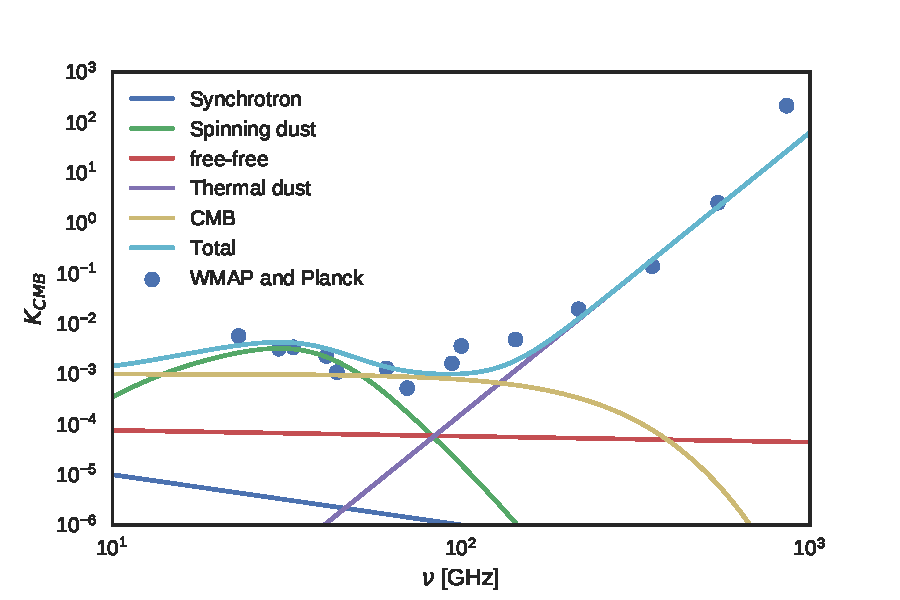
\includegraphics[width=\textwidth]{../Plots/ch_intro/mw_foregrounds_demo_rOph.pdf}
        \caption{An example of a potential makueup of microwave emission components. Photometry points are extracted from the Planck and WMAP all-sky maps, for a region well-known for prominant AME, $\rho$~Ophiuchus. \citep{planckxx11}}
      \label{fig:mw_foregrounds_demo_rOph}
    \end{figure}

    \begin{figure}
      \centering
      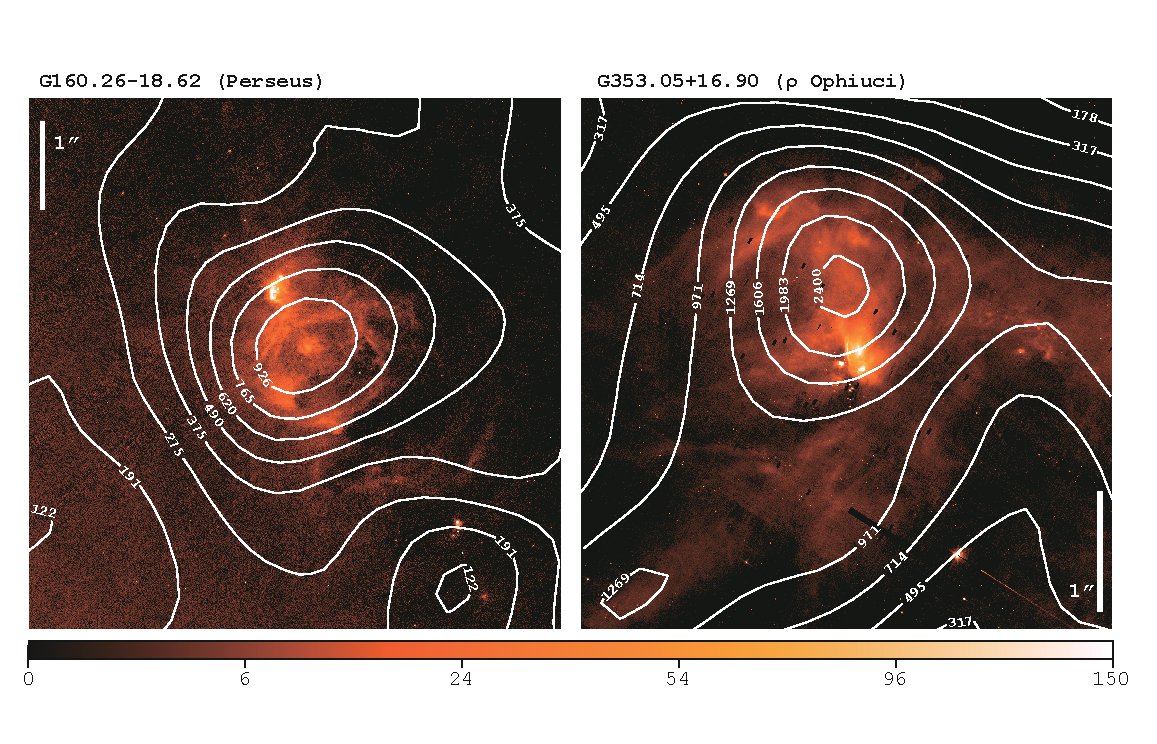
\includegraphics[width=\textwidth]{../Plots/ch_intro/AME_contours.pdf}
        \caption{Two AME prominent regions investigated by \cite{planckxx11, tibbs11}, $\rho$~Ophiuchus and Perseus, as they appear in the AKARI/IRC 9$\mu$m all-sky data at native resolution. White contours show AME at 1-degree resolution, extracted from the map by  \cite{planck15X}.}
      \label{fig:AME-contours}
    \end{figure}

    \subsubsection{Discovery and first explorations}

     Since its first detection in early microwave observations, AME has been found to be a widespread feature of the microwave Milky Way \citep{dickinson13r}. \cite{kogut96,deoliveiracosta97,leitch98} showed that the AME correlates very well with infrared emission from dust, via COBE/DIRBE and IRAS far-IR maps.
     From about 2002, the AME starts to become less of an anomaly, and more of an established albeit mysterious component of microwave emission. \cite{finkbeiner02} reported the first detection of a ``rising spectrum source at 8~to~10~GHz'' in a targeted observation, making the AME more than a statistical spectral outlier in CMB experiments. \cite{deoliveiracosta02} furher argued that this emission is in fact ``ubiquitous''. The exact mechanism and carrier/s remain mysterious however. Variations in the spectral profile of the AME signature,

     However there remains much mystery, except that the most likely source of the AME is interstellar dust. Several works have reported correlations between AME and thermal dust emission - but with some disagreement as to whether this correlation is improved in 12~$\mu$ emission vs. 100~$\mu$m emission \citep{ysard10a,tibbs11,hensley16}. Exactly which physical mechanisms are at play is still an open question, even if we assume a dusty AME origin. Even assuming a particular dust-based physical mechanism, we would still be puzzled as to the chemical composition and morphology of the carrier(s). We also lack an all-sky constraint on the emissivity of the AME spectrum at frequencies short of the WMAP cut-off, around 23~GHz.

  \subsubsection{Proposed explanations}

     From the observed spatial correlation between AME and dust emerged two prevailing hypotheses:

    1) Electric dipole emission by spinning small dust grains, a mechanism proposed in \cite{erickson57} and \cite{hoyle70}, with further discussion in \cite{ferrara94}. \cite{draine98b} give the earliest thorough description, with substantial updates contributed more recently by \cite{ysard10a}, \cite{ali-haimoud09}, \cite{hoang10} and several others. \cite{hensley17a} propose that such small spinning grains may consist primarily of silicates, and that this is allowed by observational upper-bounds of nanosilicate abudance, although nanosilicates have not yet been detected in the ISM. \cite{dickinson13r} provide a detailed overview of AME and spinning dust literature. An updated state of play of AME research has been submitted at the time of this writing (Dickinson, et al., submitted). Eq. \ref{eq:Pspin} gives the radiated power by spinning dust

        \begin{equation}
        P = {4\over9} {\mu^2\omega^4\over c^3}
        \label{eq:Pspin}
        \end{equation}

        \begin{equation}
        {\omega_T\over 2\pi} =
        \langle\nu^2\rangle^{1/2}
        \approx 5.60\times 10^9 a_{-7}^{-5/2}\xi^{-1/2}T_2^{1/2}~~~{\rm Hz}
        \label{eq:nurms}
        \end{equation}

    2) Magnetic dipole emission, caused by thermal fluctuations in grains with magnetic inclusions, proposed by \cite{draine99}.
     More recently, modeled spectra for potential candidate carriers have appeared in the literature: PAHs, grains with magnetic inclusions \citep{draine13, ali-haimoud14, hoang16a}.

    A third, but not widely accepted, possible explanation for AME is discussed in \cite{jones09}. They have suggested that the emissivity of dust, in the spectral range related to AME, could contain features caused by low temperature solid-state structural transitions.

    \subsubsection{Spinning dust}
     Spinning dust need not be the only emission mechanism, a convention as arisen in AME observational works. The photometric signature of the AME is frequently interepreted via spinning dust parameters \citep{ysard11,ali-haimoud10}. Archival all-sky AME data products exclusively assume a spinning dust SED templates.   \footnote{Both WMAP and Planck used a base template with 30~GHz peak frequency, and an assumed cold neutral medium evironment.} Using the ``spdust'' spinning dust SED model code to fit excess microwave foreground emission has become as commonplace as fitting a modified blackbody function to the far IR.

      We explore the case that the AME signature arises from spinning dust emission. If the AME is carried by spinning dust, the carrier should be small enough that it can be rotationally excited to frequencies in the range of 10-40~GHz, and must have a permanent electric dipole. Within contemporary dust SED models, only the polycyclic aromatic hydrocarbon family of molecules (PAHs), or nanoscale amorphous carbon dust fit these criteria. Those PAHs which have a permanent electric dipole (i.e. coranulene, but not symmetric molecules like coronene), can emit rotationally. However the carrier need not be carbon-based. Indeed, \cite{hensley17a} claim that AME can be explained without carbonaceous carriers, using only spinning nanosilicates.

     \subsubsection{Spinning PAHs?}
       Assuming the rotational emission model of \cite{draine98b}, the AME signature (consistent with peaked, continuum emission having a peak between 15 and 50~GHz ) implies very small oscillators (\textasciitilde{}10~nm).

       In any case, the PAH class of molecules are the only spinning dust candidate so far which show both: \\
       1) Evidence of abundance in the ISM at IR wavelengths, and \\
       2) A predicted range of dipole moments (on order of 1~debye), to produce the observed AME signature \citep{draine98b, lovas05, thorwirth07}. However, it should be noted that the current upper-bound on the abundance of nanosilicates, allows for a "spinning nanosilicate" explanation for the AME, as shown by \cite{hensley17a}. Due to the (apparently) continuous shape of the AME SED, a spinning dust explanation requires a distribution of dipole moments and/or rotational velocities of the carriers. Of course, the AME cannot simply be modeled by a distribution of carriers. Environmental factors affecting the rotational excitation of the carriers must be considered.

       \paragraph{A more testable hypothesis}
         At the time of this writing, there is no strong argument in the ltierature that either PAHs or nanosilicates are physically prefered by AME observations. The physical plausibility of rapidly spinning PAHs and of rapidly spinning nanosilicates to produce the AME have both been outlined. This plausibility however is contingent on the abundance of PAHs or nanosilicates with appropriate dipole moments, and in regions with suitable excitation environments.

         The arguments for or against particular carriers of the AME come from carrier abundance estimates and their statistical comparison with AME estiamtes. While neither nanosilicates nor any particular species of PAHs have been conclusively identified in the ISM, there is far more empiracal evidence for PAH-like dust there is for nanosilicates. Mid-infrared features associated with PAH-like aromatic materials have been observed. In fact, ``the PAH features'' are ubiquitous in the ISM \citep{giard94,onaka96,onaka00}, such that the carriers must be abundant.\footnote{ \cite{andrews15} strongly argue for the  existence of a dominant ``grandPAH'' class, containing 20 to 30 PAH species.} There has yet to be any detection of features related to nanosilicates. There is only an upper-bound from IRTS observations of \cite{onaka96} and calculations by \cite{li01}. \cite{hensley17a} argue that this upper-bound does not prohibit nanosilicates as the sole carriers of the AME.

     \subsection{Excitation factors}
       In the spinning dust model, there are several possible excitation factors for spinning dust. For the grains to have rotational velocities high enough to create the observed AME, they must be subject to strong excitation mechansisms. The dominant factors that would be giving grains their spin, are broken down by \cite{draine11} into basically two categories: 1) Collisional excitation. 2) Radiative excitation, the sum of which could lead to sufficient rotational velocities for sufficiently small grains. However the extent of excitation will depend on environmental conditions, i.e. there will be more frequent encounters with ions and atoms in denser regions (so long as the density is not high enough to coagulate the small grains), and more excitation due to photon emission with increasing ISRF strength \citep{ali-haimoud09, ali-haimoud14}. One of the strongest potential excitation mechansims listed in \cite{draine11} is that of negatively charged grains interacting with ions. Thus not only must we consider environmental factors, grain composition and size, but also the ionization state of the carriers. (For example, ionizaed vs. neutral PAHs.) The dependence of the observed AME on ISM density is modeled by \cite{ali-haimoud10}, demonstrating that denser regions may have a stronger AME component (although it can be observationally challenging to resolve dense vs. diffuse AME producing regions.)

       \subsection{AME vs. IR in the literature}
          The overall pattern among large-scale studies seems to show that all of the dust-tracing photometric bands correlate with the AME (and each other) to first-order.  On an all-sky, pixel-by-pixel basis, at 1$^{\circ}$ angular resolution, \cite{ysard10b} find that 12~$\mu$m emission, via IRAS, correlates slightly more strongly with AME (via WMAP) than with 100~$\mu$m emission.  They also find that scaling the IR intensity by the interstellar radiation field strength (given as $G_0$, a measure of ISRF relative to that of the solar neighborhood) improves both correlations. THey interpret this finding as evidence that AME is related to dust, and more closely related to the small stochastically emitting dust that is traced by 12~$\mu$m emission.

          However in a similar work, \cite{hensley16} report that the 12~$\mu$m emission (via WISE) correlates less tightly with AME than with thermal dust radiance, using the Planck Collaboration dust and AME component-separation maps \citep{planck15X}. Also at odds with \cite{ysard10b}, they report that AME correlates more strongly with 12~$\mu$m intensity than with the intensity scaled by the interstellar radiation field. They interpret this as AME and PAH emission both being correlated with the total dust radiance, but that there is no preferential relationship between PAHs and the AME.

         The story is no more clear when looking at the average properties of individual regions. \cite{planckXV} find that among 22 high-confidence ''AME regions" (galactic clouds such as the $\rho$~Ophiuchus cloud and the Perseus molecular cloud complex) AME vs. 12~$\mu$m  shows a marginally weaker correlation than AME vs. 100~$\mu$m (via IRAS). \cite{tibbs11} examined the AME-prominent Perseus Molecular Cloud complex, finding that while there is no clear evidence of a PAH-AME correlation, they do find a slight correlation between AME and  $G_0$.

          %       In this work, we attempt to reach some stronger consensus on the large-scale AME vs. IR-dust story, keeping in mind that resolution limitations are a could dilute more subtle connections between potential connections between dust IR emission and the anomalous foreground. In Ch. \hyperref[ch:datasources]{\ref*{ch:datasources}}, we describe the all-sky surveys and component maps used in this paper. The sources range from PAH-domianted MIR bands from AKARI and IRAS to FIR and microwave-derived maps from Planck Observatory. These bands are listed in Tab. \ref{tab:data} and are described in \ref{ch:datasources}. Our investigation is broken into two major approaches: a localized study of a particularly interesting AME region, around $\lambda$ Orionis, and an exploration into all-sky trends, to see if $\lambda$ Orionis results can be generalized. Chapter  \hyperref[ch:discussion]{\ref*{ch:discussion}} describes the conclusions of these 2 approaches, and compares them to previous AME vs. dust emission studies.

\section{Scope of this Dissertation}

  \subsection{An application of all-sky archival data}
    This is an astrophysical data archive based work. The primary goal is to highlight a particular application of multiwavelength (mid-IR to radio), cross-archive all-sky data analysis. We describe the interrelatedness between mid to far IR dust emission and possible microwave emission from dust. This is accomplished through an investigation of photometric all sky maps mainly from AKARI, IRAS, and Planck.

  \subsection{Testing the spinning PAH hypothesis}
    For the present work, we consider the spinning PAH hypothesis to have the highest degree of testability, due to the well-established presence of aromatic emisison feaetures in the ISM.  We do not argue against the physical plausibility of nanosilicates to produce the AME. Indeed, there is no argument to date that these potential physicalities are mutally exclusive, as long as both potential carriers are sufficiently abundant. Nor does spinning dust emission theoretically exclude magnetic dipole emission or microwave thermal dust emissivity fluctuations.

  \subsection{Limitations}
    We do not explore the modeling of microwave dust emission itself, rather the comparison of existing archival data and parameter maps. Modeling of the exact physical mechanism of the anomalous component of galactic microwave foreground emission from first principles is beyond the scope of this work. We consider this problem first on an all-sky basis, not focusing on any pre-selected object of the sky - in order to assess if there any general pattern between the IR and the AME, beyond the AME-dust correlation already described above. We then focus on a region highlighted by the Planck Collaboration as being especially worthy of further investigation \citep{planck15X}, and has a resolvable topology even at 1-degree resolution. Essentially all of the analyses and conclusions presented in this work apply to an angular scale of approximately 1-degree, and only for the given component separation methods (Solar system, galactic, extragalactic) used by each of the data providers.

  \subsection{Code availability}
    This dissertation is accompanied by a github repository\footnote{Available at: \url{https://github.com/aaroncnb/CosmicDust}.} Virtually all of the analyses code are available in that repository, in the form of Jupyter notebooks (along with the figures and the code used to generate them.) The dust SED fitting code is not part of that reposittory, but is described in Galliano et al. (in prep.)


\chapter{Data Sources}
  \label{ch:datasources}

  \section{A collection of skies}
    This work relies completely on all-sky surveys. All of the maps utilized are photometric-band infrared maps, except for the AME data, which is an all-sky component separation analysis product, from the Planck Collaboration's efforts to separate galactic foregrounds from the CMB. Table~\ref{tab:data} summarizes the observational data used in this thesis.
    \begin{table}[h]
      \caption{Observational data sources used in this article}
      \centering
        \begin{tabular}{lrrrrr}
        \hline\hline
        Instrument & Central Wavelength & FWHM & Cali & Reference \\
        \hline
        AKARI/IRC & 9~$\mu$m  &  \textasciitilde{}10$"$ & \textless 10\%   & \tablefootnote{\cite{ishihara10}} \\
        AKARI/IRC & 18~$\mu$m & \textasciitilde{}10$"$  & \textless 10\%     & '' \\
        AKARI/FIS & 65~$\mu$m  & 63$"$ & \textless 10\% & \tablefootnote{\cite{doi15,takita16}} \\
        AKARI/FIS & 90~$\mu$m  & 78$"$ & \textless 10\%   & '' \\
        AKARI/FIS & 140~$\mu$m & 88$"$ & \textless 10\%   & '' \\
        AKARI/FIS & 160~$\mu$m & 88$"$ & \textless 10\%   & '' \\
        IRAS/IRIS & 12~$\mu$m   & 4.0$'$ &   \textless 5.1\%       & \tablefootnote{\cite{iris05}} \\
        IRAS/IRIS & 25~$\mu$m   & 4.0$'$ &    \textless 15.1\%      & ''\\
        IRAS/IRIS & 60~$\mu$m   & 4.2$'$ &    \textless 10.4\%      & '' \\
        IRAS/IRIS & 100~$\mu$m  & 4.5$'$ &   \textless 13.5\%       & '' \\
        Planck/HFI & 345~$\mu$m & 4.7$'$ & & \tablefootnote{\cite{hfi14viii}} \\
        Planck/HFI & 550~$\mu$m & 4.3$'$& & '' \\
        \hline
         \label{tab:data}
      \end{tabular}
    \end{table}
    In total, we employ all-sky maps from 12 photometric bands, spanning the wavelength range of 6.9~$\mu$m to 550~$\mu$m as showin in Fig.~\ref{fig:Filter_coverage_example_full} The following sections give the details of the observational data from each instrument as well as of the parameter maps provided in \cite{planck15X}.\footnote{Planck bands are named according to their central frequency, not wavelength.}
      \begin{figure}
        \centering
        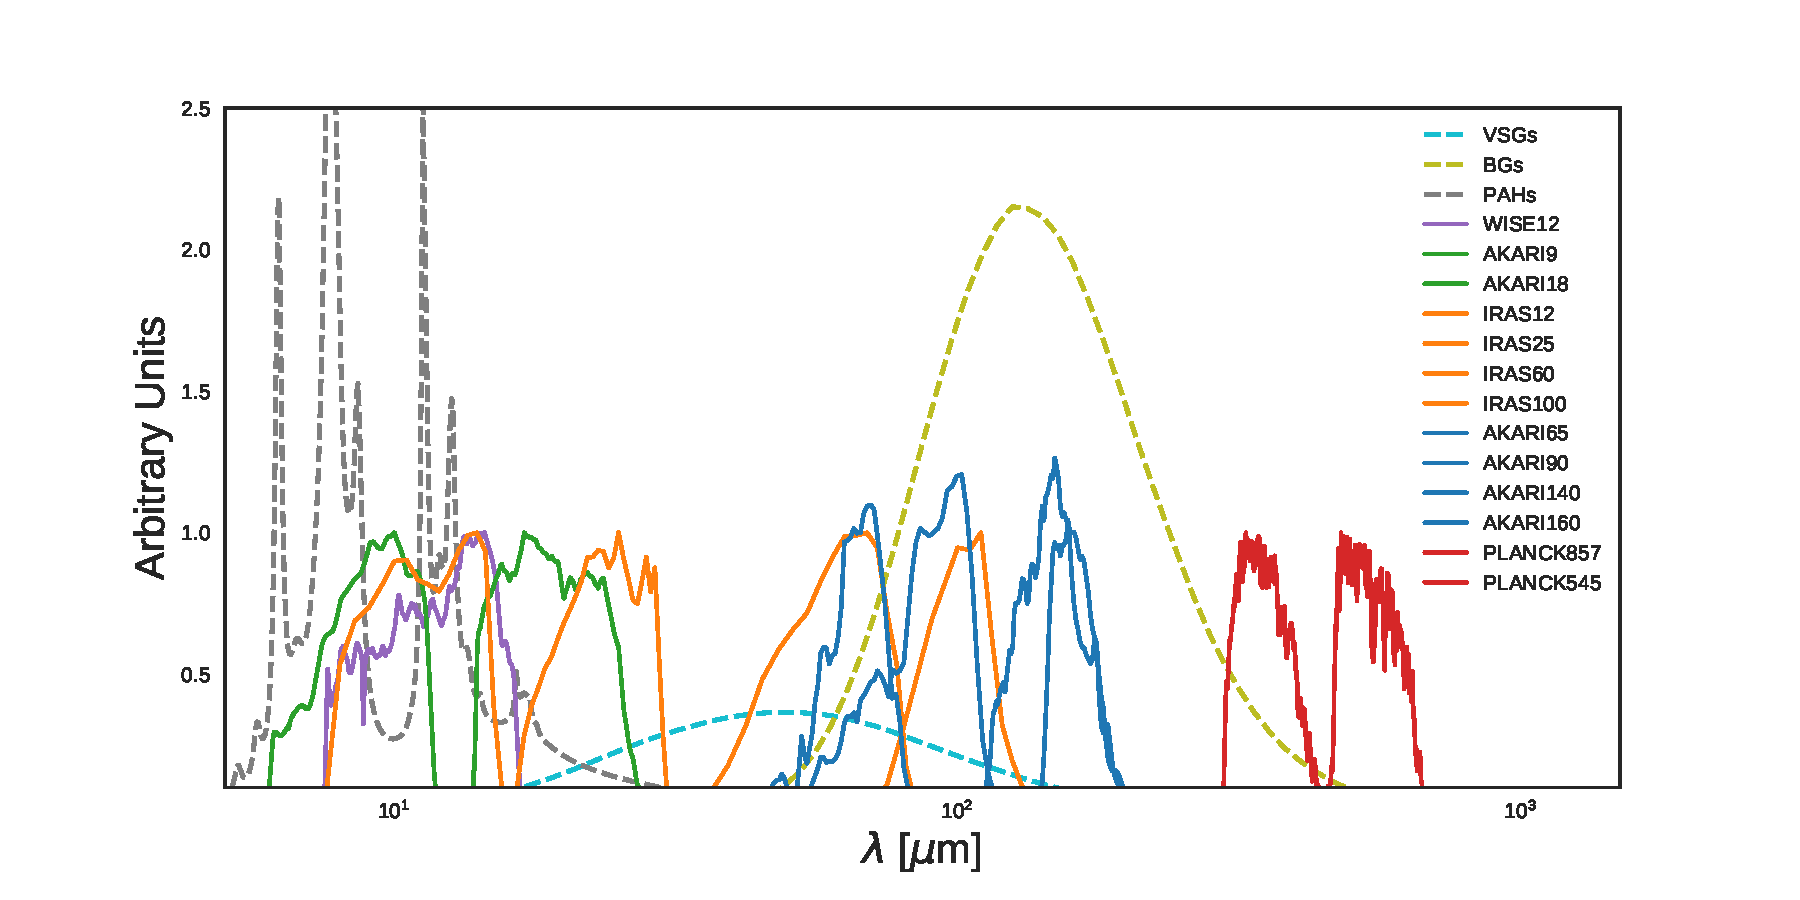
\includegraphics[width=\textwidth]{../Plots/ch_datasources/Filter_coverage_example_full.pdf}
        \caption{Relative spectral response curves of the bands used in this study. Expected dust emission components, assuming the dust SED model by \citep{dustem11} are also shown. The components are summarized as emission from big grains (BGs, dashed yellow line), emission from very small grains (VSGs, dashed blue line), and emission from PAHs (dashed grey line).}
        \label{fig:Filter_coverage_example_full}
      \end{figure}
    From this point in the thesis, we will mostly use abbreviations to refer to the different bands, as follows: 'A' indicates AKARI; 'D', DIRBE; 'I', IRAS, and 'P' Planck. The number after each letter indicates the band central nominal wavelength in microns (or frequency in GHz, in the case of the Planck bands.)
    \begin{table}[h]
      \caption{Ancilliary data}
      \centering
        \begin{tabular}{lrrrr}
        \hline\hline
        Product   & Relevant Freq./Wavelen  & FWHM    & Reference/URL \\
        \hline
        $H\alpha{}$  & 658.5~nm  & 36$'$  & \tablefootnote{\cite{finkbeiner03}: \\ \url{https://lambda.gsfc.nasa.gov/product/foreground/halpha_map.cfm}} \\
        $N(H)$       & 21~cm     & 36$'$  & \tablefootnote{\cite{kalberla05}: \\ \url{https://lambda.gsfc.nasa.gov/product/foreground/fg_LAB_HI_Survey_get.cfm}} \\
        PC $R$ (PR1)          & 353~GHz   & 5$'$   & \tablefootnote{\cite{}: \\ \url{http://irsa.ipac.caltech.edu/data/Planck/release_1/all-sky-maps/previews/HFI_CompMap_ThermalDustModel_2048_R1.20/index.html} }\\
        PC $\tau_{353}$ (PR1) & 353~GHz   & 5$'$    & '' \\
        Haslam~MHz   & 408~MHz   & 56$'$  & \tablefootnote{\cite{haslam82}: \\} \\
        PC Synchrotron (PR2) & 408~MHz & 60$'$ & \tablefootnote{\cite{planck15X}: \\ \url{http://irsa.ipac.caltech.edu/data/Planck/release_2/all-sky-maps/previews/COM_CompMap_Synchrotron-commander_0256_R2.00/index.html}} \\
        PC $AME_{var}$ (PR2) & 22.8~GHz & 60$'$ & \tablefootnote{\url{http://irsa.ipac.caltech.edu/data/Planck/release_2/all-sky-maps/previews/COM_CompMap_AME-commander_0256_R2.00/index.html}} \\
        PC $AME_{fix}$ (PR2) & 41.0~GHz & 60$'$ & '' \\
        PC free-free (PR2) & N/A & 60$'$ & \tablefootnote{\url{http://irsa.ipac.caltech.edu/data/Planck/release_2/all-sky-maps/previews/COM_CompMap_freefree-commander_0256_R2.00/index.html}} \\
        \hline
         \label{tab:ancilliarydata}
      \end{tabular}
    \end{table}

  \section{AKARI}
  \label{sec:AKARI}
       The AKARI infrared space telescope revealed an entire sky of infrared light, from the mid to far infrared, via two instruments \citep{akari07} the Infrared Camera (IRC)\citep{irc07} and the Far Infrared Surveyor (FIS) \citep{fis07}. In this section we will discuss the all-sky surveys produced by these two instruments.
       \subsection{AKARI/Infrared Camera (IRC) }
           IRC proivded us with both spectroscopic and phometric data from the near to mid-infrared. In this work, we utilize the all-sky maps centered at 9 and 18~$\mu$m, created during by the IRC's fast-scanning mode. We utilize the most recent version of the IRC data (Ishihara, et al., in prep.) This version has had an updated model of the Zodiacal light, fitted and subtracted. The details of the improved Zodi-model, which offers an improvement over that used for the IRAS all-sky maps, are given in \cite{kondo16}.
       \subsubsection{PAH feature coverage}
         The A9 all-sky map demonstrates the abundance of the PAH bands carrier in the Milky Way \citep{ishihara10}. Figure~\ref{fig:Filter_coverage_example_PAH} shows the coverage of the PAH features (from both ionized and neutral PAH components), as they are theoretically determined in \cite{dustem11}.
            \begin{figure}
              \centering
              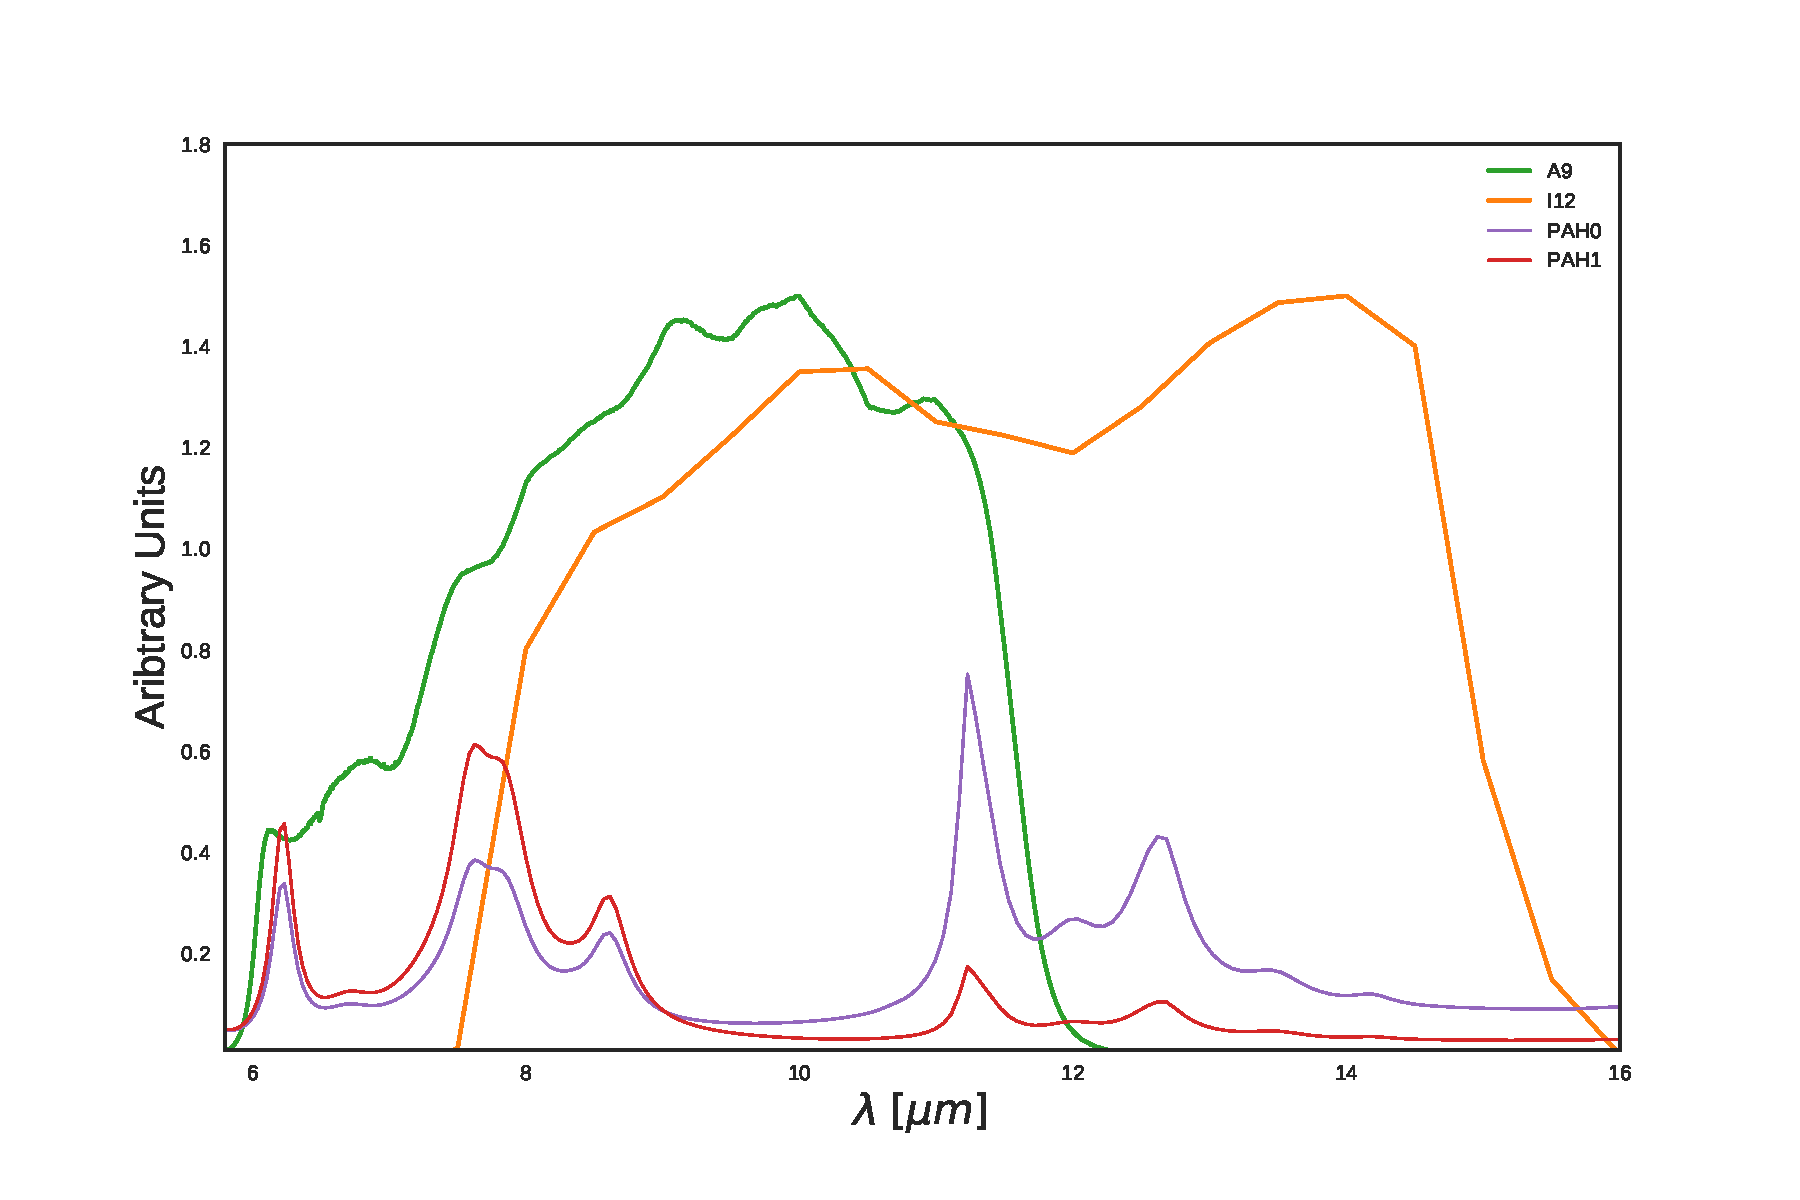
\includegraphics[width=\textwidth]{../Plots/ch_datasources/Filter_coverage_example_PAH.pdf}
              \caption{The I12 (orange) and A9 (green) filters coverage of modeled ionized (PAH1, red) and neutral (PAH0, purple)components of PAH features by \cite{dustem11}. The difference in the PAH feature coverage mainly comes from the 6.2~$\mu$m and the 7.7~$\mu$m feature.}
              \label{fig:Filter_coverage_example_PAH}
            \end{figure}
         The A9 band uniquely covers major ionized PAH features at 6.2 and 7.7~$\mu$m; as well as neutral PAH features at 8.6 and 11.2~$\mu$m across the entire sky \citep{irc07}. The I12 band covers the 11.2 and 8.6~$\mu$m features, and the similarly-shaped W12 band covers primarily the 11.2~$\mu{}$m feature but do not cover the 7.7~$\mu{}$m completely. According to the distribution of PAH features across the response filters in Fig.~\ref{fig:Filter_coverage_example_PAH}, and referring back to the various dust components in Fig.~\ref{fig:Filter_coverage_example_full} it is also expected that the A9 band is most dominated by PAH emission even with increasing $U$. This may seem counter-intuitive, since, as described in Ch.~\ref{ch:intro}, the PAH spectral shape does not show a temperature variation. However as $T$ increases, the MIR extent of thermal dust emission and emission from VSGs encroach on I12 and WI2 sooner than A9, diluting emission from PAHs. In some ionized reigons, I12 may also include non-significant contributions from the [NeII] line at 12.8~$\mu$m. Figure~\ref{fig:Filter_coverage_example_MIR} demonstrates an example observational galactic cirrus spectrum in the MIR, from Spitzer Infrared Spectrograph (IRS) \citep{spitzer04} data, along with filters for all of the MIR bands used in this study.
             \begin{figure}
               \centering
               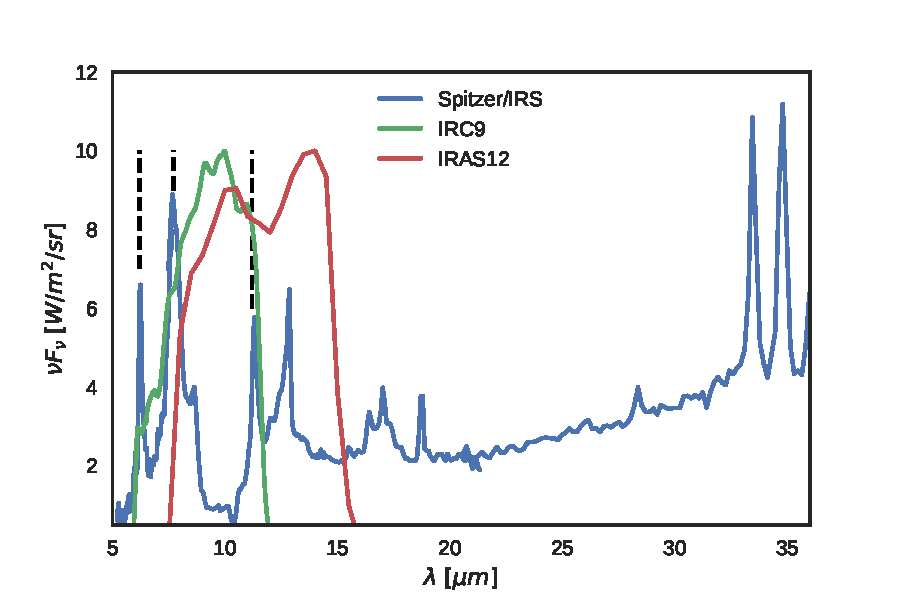
\includegraphics[width=\textwidth]{../Plots/ch_datasources/Filter_coverage_example_MIR.pdf}
               \caption{Coverage of MIR wavelengths by the filters used in this work. An Spitzer/IRS spectrum (see AOT4119040) of the galactic plane (thin blue line) demonstrates how IRC and IRAS photometric bands trace these features on an all-sky basis \citep{ishihara07}. Strong PAH features overlap with the A9 and I12, while the A18 and I25 micron bands only trace much weaker features. }
               \label{fig:Filter_coverage_example_MIR}
             \end{figure}
         It indicates that the other MIR bands, A18 and I25, do cover strong PAH features and are expected to be dominated rather by emission from very small grains (VSGs), as was indicated in Fig.~\ref{fig:Filter_coverage_example_full}.

         To help demonstate how the relative contribution from PAHs will change for each band, for different ISRF strengths, Fig.~\ref{fig:InBandFracContribution_PAH} gives just such a calculation. These contributions remain relatively constant out to a $U$ of about 100, with the contribution from warm dust becomming a larger factor for the I12 and W12 bands. Thus, according to the DL01 template, A9 should have the highest contribution from PAHs out to extreme radiation fields. At least to the extent with which PAHs can endure harsh UV radiation, as PAHs are expected to evaporate in strong enough radiation fields \citep{allain96a,allain96b,bocchio12,pilleri12, pavlyuchenkov13}.

      \subsubsection{PAH ionization}
        Figure~\ref{fig:Filter_coverage_example_PAH} indicates that expected emission from ionized PAHs may preferentially contribute to the A9 band, even though both I12 and A9 cover ionized and neutral features. A PAH SED model calculation, using the \cite{dustem11} SED template, supports that for Galactic cirrus ISM conditions, emisison detected by the A9 band would have a higher contribution from charged PAHs than the I12 band. This is demonstrated in Fig.~\ref{fig:InBandFracContribution_PAH}.
          \begin{figure}
              \centering
              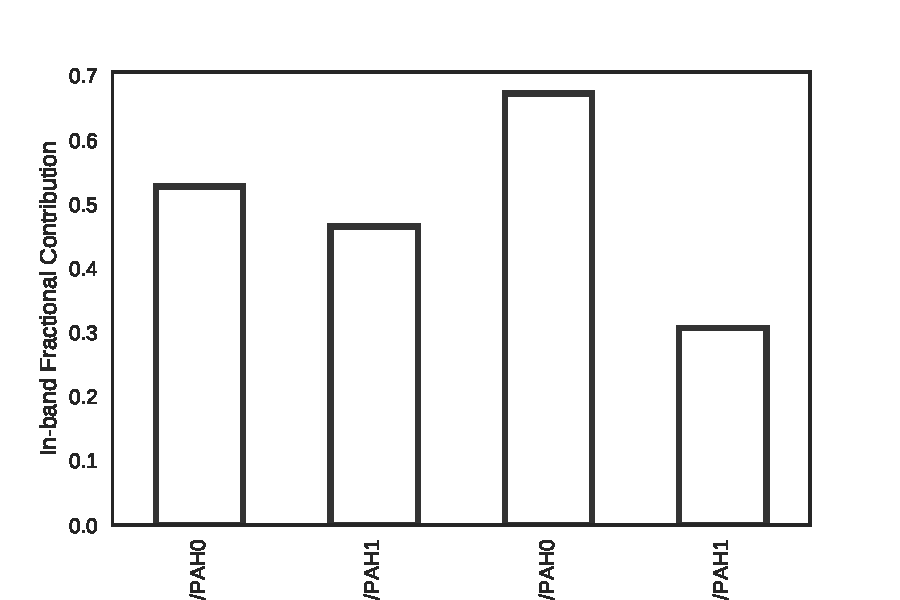
\includegraphics[width=\textwidth]{../Plots/ch_datasources/InBandFracContribution_PAH.pdf}
              \caption{In-band contributions from charged (PAH1) neutral (PAH0) PAHs, to the emission detected by the I12 and A9 filters. These assume a model galactic cirrus spectrum simulated with the SED template of \cite{dustem11}. }
              \label{fig:InBandFracContribution_PAH}
          \end{figure}
        To be clear, both bands are sensitive to both charged and neutral PAHs, however the relative contribution from charged PAHs is expected to be higher for A9. Thus we might expect that the ratio of intensities in this two bands, for a given line of sight (towards which PAHs are not destroyed), could trace the fraction of charged PAHs. Estimating the extent of this effect, Fig.~\ref{fig:band-ratio-multiple} gives the results of a calculation of I12/A9 and I25/A9 band ratios for two ISRF strengths.
          \begin{figure}
              \centering
              
\includegraphics[width=\textwidth]{../Plots/ch_datasources/band-ratio-multiple.pdf}
              \caption{Ionization fraction of PAHs vs. band ratios of I12, I25, to A9, for two ISRF strengths: Top: $U = 1$, Bottom: $U = 10$. These ratios are determined by assuming the SED template of \cite{dustem11} }
              \label{fig:band-ratio-multiple}
          \end{figure}
        This calculation is again based on \cite{dustem11}. It suggests that at least for $U<\sim{}10$, the fraction of charged PAHs may be estimated as a function of the I12/A9 ratio.

         Examing how this might look in the data themselves, Fig.~\ref{fig:ratioMap_A9I12} and Fig.~\ref{fig:ratioMap_A9I25} show the R(A9:I12) and R(A9:I25) ratio maps, demonstrating the relative variations in these MIR bands accross the sky--- or at least the portions of the sky where S/N is sufficient. While from visual inspection the various MIR intensity all-sky maps appear to essentially trace the same stuctures of the galaxy, the ratio maps reveal that there are indeed differences to be explored.  In regions where noise is dominant, ascertaining the ionization fraction will be quite difficult. This can be easily seen upon visual inspection of the ratio maps, in that there is a clear deliniation between brighter emission towards lower galactic latitudes, and the high latitude sky where the ratio shows very little discernible structure (except for the Zodi-residual patterns which differ between IRC and IRAS.) Thus there may a large portion of the sky where the S/N may be high enough to allow us to trace the PAH ionization fraction. This possibility is explored in Ch.~\ref{ch:lori}, in looking at the PAH distribution within $\lambda$~Orionis.
             \begin{figure}
               \centering
               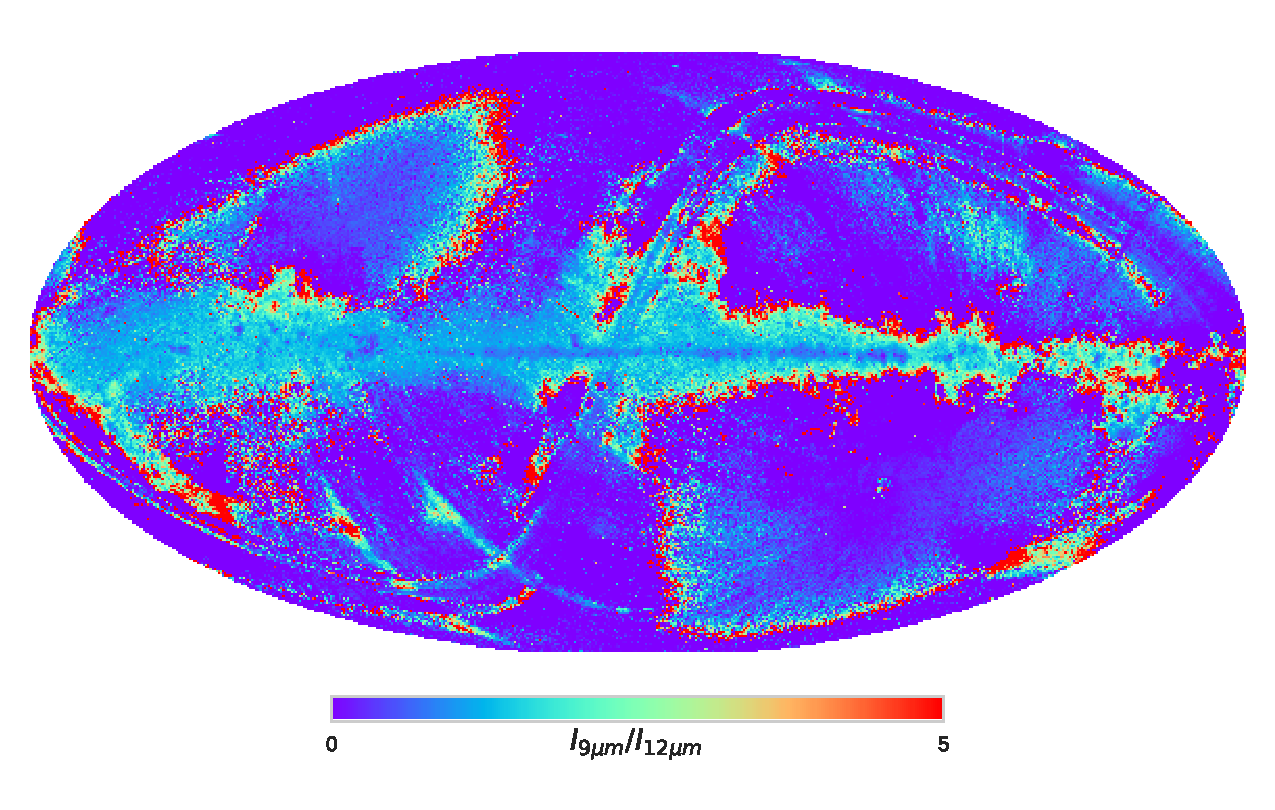
\includegraphics[width=\textwidth]{../Plots/ch_datasources/ratioMap_A9I12.pdf}
               \caption{ AKARI/IRC 9~$\mu$m to IRAS 12~$\mu$m intensity ratio.}
               \label{fig:ratioMap_A9I12}
             \end{figure}
             \begin{figure}
               \centering
               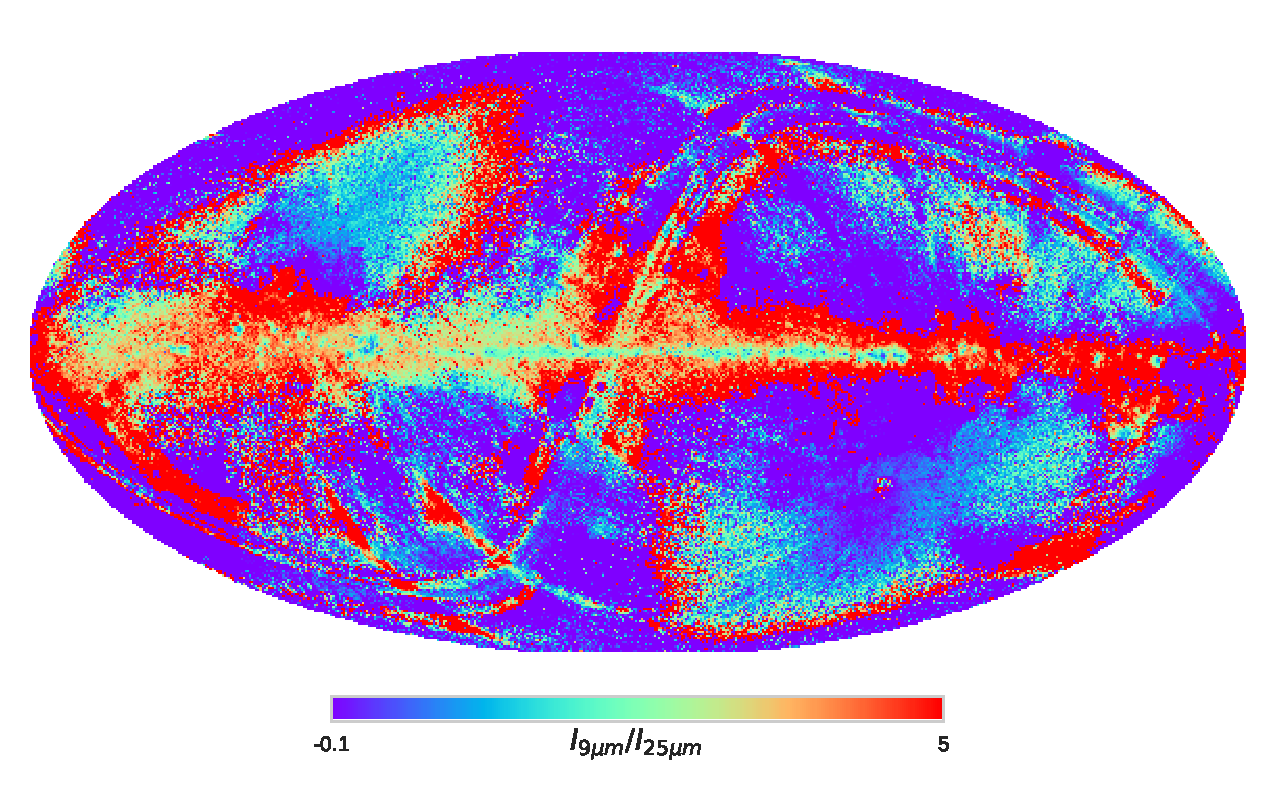
\includegraphics[width=\textwidth]{../Plots/ch_datasources/ratioMap_A9I25.pdf}
               \caption{ AKARI/IRC 9~$\mu$m to IRAS 25~$\mu$m intensity ratio.}
               \label{fig:ratioMap_A9I25}
             \end{figure}

    \subsection{The AKARI Far Infrared Surveyor (FIS)}
       FIS gives us photometric data around the peak of the typical thermal dust SED. FIS was equipped with four wavebands: two narrow bands centered at 65~$\mu$m and at 160~$\mu$m, and two wide bands at 90~$\mu$m and at 140~$\mu$m. An all-sky survey was carried out at each band \citep{kawada07}, and the processed maps have been publicly released \citep{doi15}.

    \subsection{Planck Observatory High Frequency Instrument (HFI)}
       The HFI all-sky maps, spanning 100 to 857~GHz \citep{hfi14viii} help constrain the far IR dust emissivity. This study utilizes the 857~GHz (345~$\mu$m) and 545~GHz (550~$\mu$m) bands.

    \section{Infrared Astronomical Satellite (IRAS)}
       Data from the IRAS \citep{iras84} all-sky surveys are used to supplement the similarly-centered AKARI photometric bands. The IRAS 12~$\mu$m band is similar to the IRC 9~$\mu$m band in terms of the sky coverage, central wavelength, and especially in that both surveys are heavily dominated by zodiacal light. We use the Improved Reprocessing of the IRAS Surveys (IRIS) \citep{iris05}, which have undergone a zodiacal-light removal. The zodiacal light model, however differs between the two bands. The IRAS zodi-subtraction is primarily based on the \cite{kelsall98} model, while IRC employs a modified version of this model \citep{kondo16}. Although WISE provides higher resolution than IRAS, we do not utilize the WISE data because we found the WISE all-sky 12~$\mu$m product to essentially trace the Planck HFI 857~GHz map, at 1$^{\circ}$ angular resolution. \cite{hensley16} had noted that this scaling of the WISE map may artificially suppress actual PAH-related variations at low resolution. Moreover, since we are conducting our analysis at 1$^{\circ}$ resolution in order to match the AME data, the higher resolution offered by WISE is not a significant advantage.

  \section{Planck COMMANDER Parameter Maps}
  \label{sec:PCmaps}
       We utilize the COMMANDER-Ruler astrophysical component separation maps \citep{planckXII}, from the Planck Collaboration's Public Data Release 2 (hereafter, PR2)\citep{planck2015I}. These contain estimates of known microwave foreground components (free-free, synchrotron, thermal dust emission contributions to the Planck photometric bands. Fig.~\ref{fig:PCCS_corrmatrix} demonstrates the correlatedness of these component maps, taken as provided in the PR2 archive.
         \begin{figure}
           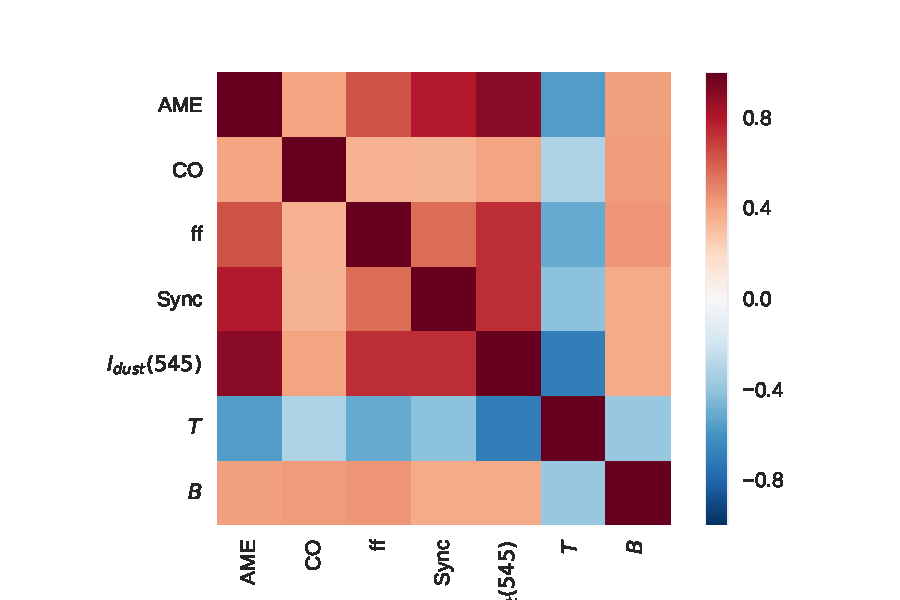
\includegraphics[width=\textwidth]{../Plots/ch_datasources/PCCS_corrmatrix.pdf}
           \centering
           \caption{$r_{s}$ cross correlation matrix of the PCCS maps: temperature $T$, emissivity index $\beta$, and amplitude at 545~GHz $I_{dust}(545)$ of thermal dust; intensity of free-free emission $ff$ at ; intensity of synchrotron emisison at 4~MHz $Sync$; intensity of the AME var. freq. component $AME$ at 22.8~GHz.}
           \label{fig:PCCS_corrmatrix}
         \end{figure}
        Without considering noise levels or variations of scale, we see evidence these major components are correlated with one another. In the case of free-free emission,  \cite{vonHausegger15} found that by taking S/N ratios into account, the correlation between COMMANDER free-free and AME components turns negative. More generally they suggest that the intercorrelations betwen these products varies with scale. We will first describe the 'non-AME' components, so as to not give any indiciation that their estimation is trival.

       \subsection{Synchrotron}
          While the Planck observations themselves do limit our resolution when assessing the AME - it is the primary constraint on synchrotron emission, 408~MHz map by \cite{haslam82} that is the major resolution limiting factor. While an impressive early effort to reveal the low-frequency sky, \citep{haslam82} is limited to an approximately 1$^{\circ}$ resolution. The map also contains many artifacts. For the time being however, it is still the most synchrotron-dominated all-sky map available, and for this reason PC15X included it in their COMMANDER component separation. Enhanced synchrotron mapping efforts are currently in progress by the `The final synchrotron product produced by COMMANDER (hereafter, PCSync) highly resembles the \cite{haslam82} map, however it is also demonstrated PCSync does not fully capture the synchrotron signal. This can be visualized by inspecting the PCAME:PCdust ratio map (see Fig.~\ref{fig:R_PCAMEtoPCdust}), which \cite{hensley16} describe as containing synchrotron emission patterns at high latitudes.

       \subsection{Free-free emission}
          Unlike the PCSync component, the fitting of the Planck COMMANDER free-free component map (hereafter, PCff) does not employ any free-free dominated emisison map, even though an earlier Planck AME paper \citep{planckXV} had employed the $H\alpha$ map by \cite{finkbeiner03}. Uncertainties in this map arise from uncertainties in the gas temperature, and the Gaunt factor. This emission source is the dominant source of confusion with AME, especially for HII regions \citep{planckXV,planckXII, paladini15}.

      \subsection{Thermal dust emission}
      ``Thermal dust emission'' in the COMMANDER context refers to dust emission in the Rayleigh Jeans-regime, as the COMMANDER fitting includes neither photometric constraints on the thermal emission peak, nor on Wiens-regime emission from small grains. This component essentially involves the fitting of a modified blackbody curve (Eq.~\ref{eq:mbb}.) to the Planck Photometry. This approach however results in an apparent anti-correlation between $\beta$ and $T$ (Fig.~\ref{fig:PCCS_corrmatrix}). Whether or not this anti-correltion is genuine is still unsettled in the literature \citep{galliano11,juvela12}. In any case, we do not utilize the $\beta$ and $T$, only the dust intensity at 545~GHz~($I_{d}$) parameter map.

      \subsection{AME data}
          The COMMANDER map release also provides an ``AME component map'', which presumes that AME originates from spinning dust. While acknowledging that such a decomposition lacks a strong physical interpretation, \cite{planck15X} break the AME into two components: a spatially varying peak frequency component, $AME_{var}$, and a spatially constant peak frequency component, $AME_{fix}$. As seen in Fig.~\ref{fig:AME_commander_freqdist}, virtually all of the fitted peak frequncies for $AME_{var}$ are beyond the reach of WMAP and Planck.
              \begin{figure}
                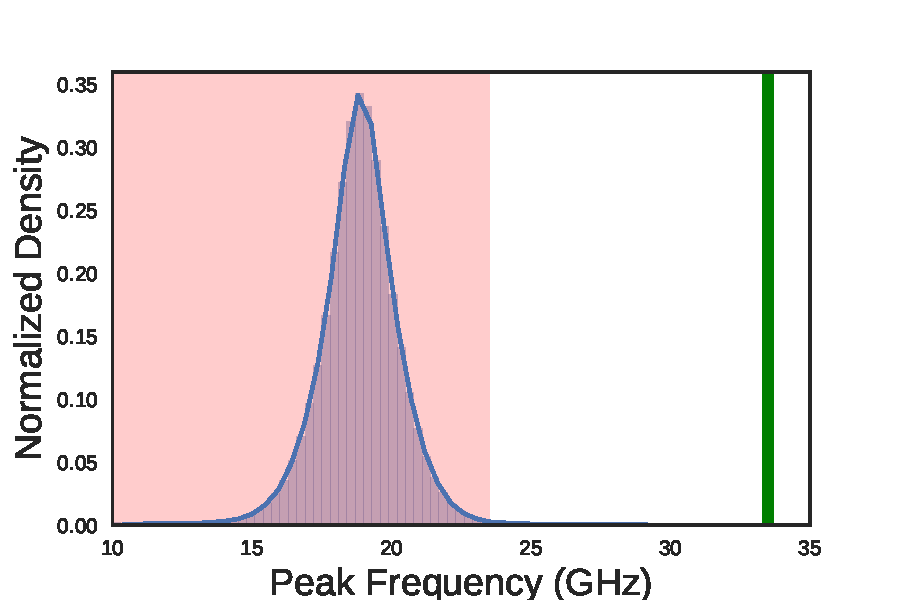
\includegraphics[width=\textwidth]{../Plots/ch_intro/AME_commander_freqdist.pdf}
                \centering
                \caption{The peak frequencies of the varying component $AME_{var}$.  The pink shaded region indicates frequencies not covered by either WMAP or Planck The green line at 33.5~GHz indicates the peak frequency of $AME_{fix}$.}
                \label{fig:AME_commander_freqdist}
              \end{figure}
          Only the fitted global frequency, 33.5~GHz for the spatially constant component, is covered. However they note that the combined components, per pixel, would have an average peak  at least within the WMAP coverage range. In any case, we stress that while this is the most careful all-sky attempt to isolate the AME to date, the constraints of the the frequency peak are still heavily lacking. In general, $AME_{var}$ is the dominant component, accounting for approximately 90\% of the total fitted AME intensity between 20 and 40~GHz, indicated by the full-sky histograms in Fig.~\ref{fig:AME_comps_distplot}.
              \begin{figure}
                 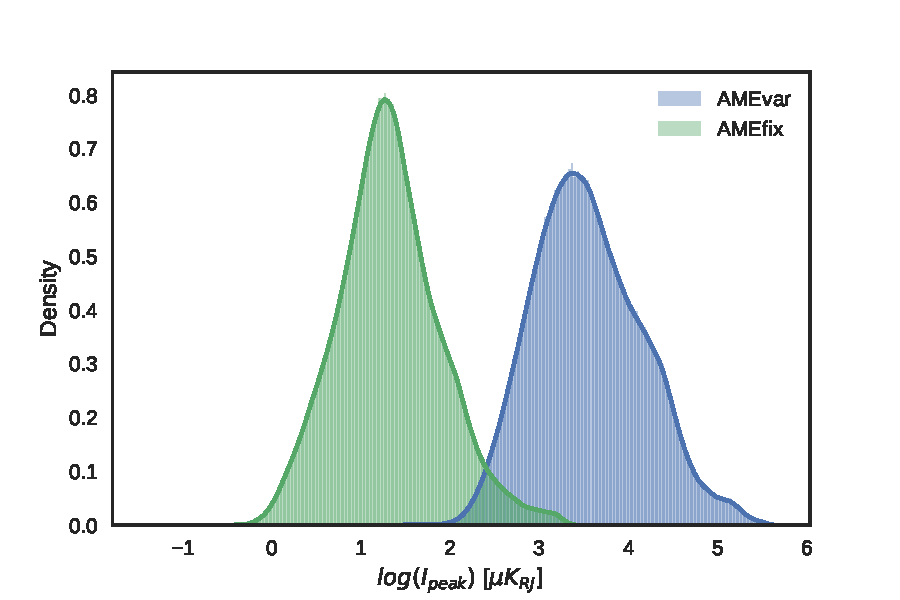
\includegraphics[width=\textwidth]{../Plots/ch_datasources/AME_comps_distplot.pdf}
                 \centering
                 \caption{Histograms of the peak intensity AME maps calculated from the original COMMANDER-AME reference frequency maps. The dominant component, $AME_{var}$ is indicated in blue, for all pixels in the map, with their spinning dust intensities evaluated their peak frequencies (see Fig.~\ref{fig:AME_commander_freqdist}.) $AME_{fix}$ gives the peak intensity of the spatially-constant frequency component, indicating it is essentially always the weaker component.}
                 \label{fig:AME_comps_distplot}
              \end{figure}
           The intensities given by PC are evaluated at reference frequencies: 22.8~GHz for $AME_{var}$, 41~GHz for $AME_{fix}$ (for convenient comparison to the WMAP total intensity maps at those frequencies). They are not fitted peak intensities of the spinning dust SED model.

            While acknowledging that the frequency constraints are lacking, we choose  to use these parameters maps in a self-consistent way, by taking the intensities and frequencies given by PC, and calculating the implied peak intensity. In any case, we find that this conversion does not have a significant effect on the results in the chapters to follow, except in the case of some outlying pixels with very low peak frequencies, easily seen in the map of the fitted frequencies in Fig.~\ref{fig:PCAME_var_freq}. .
               \begin{figure}
                 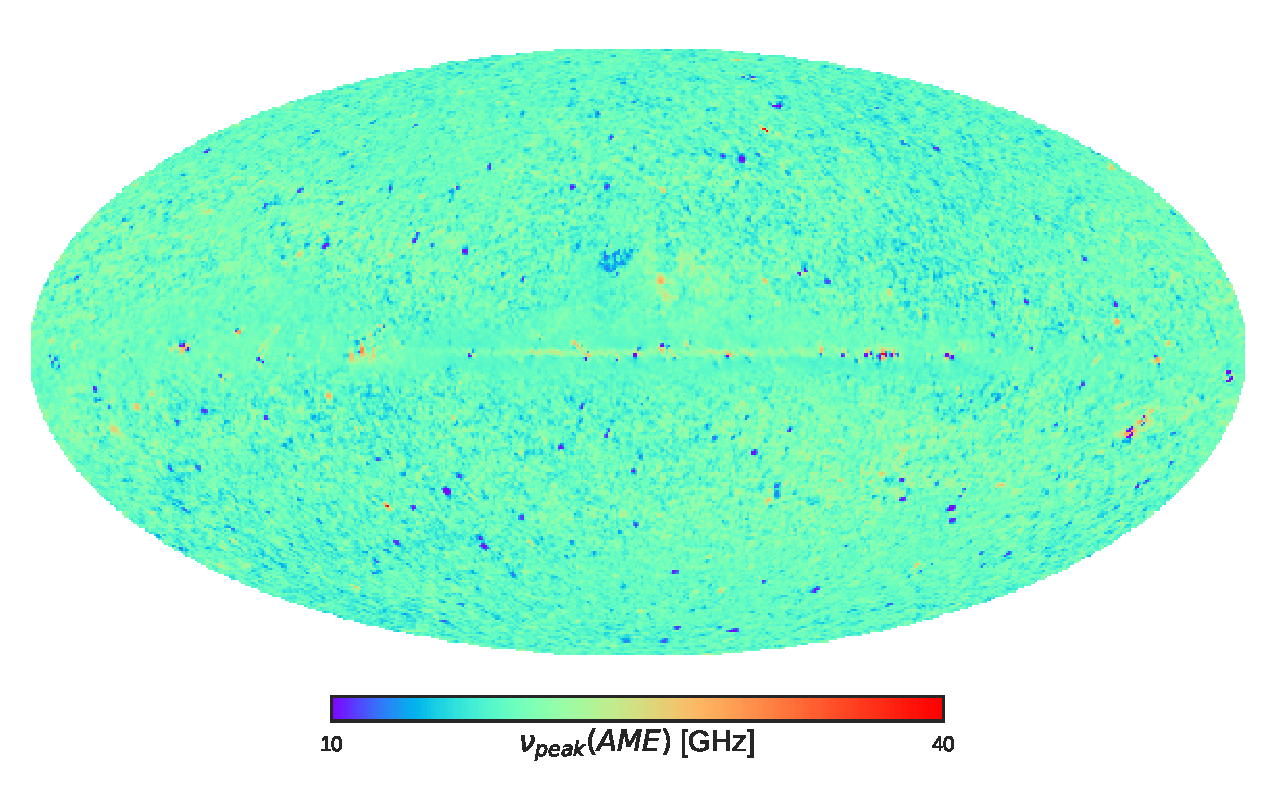
\includegraphics[width=\textwidth]{../Plots/ch_datasources/PCAME_var_freq.pdf}
                 \centering
                 \caption{All-sky map of the peak frequencies of the varying component $AME_{var}$, corresponding to Fig.~\ref{fig:AME_commander_freqdist}. Virtually all of the purple regions of the map correspond to pixels flagged for point sources in the LFI data. There are very few notable structures in the frequency map overall, other than the galactic plane itself, $\rho$~Ophiuchus, and Perseus.}
                 \label{fig:PCAME_var_freq}
               \end{figure}
               These low frequency pixels result in very high AME peak intensities.    On comparison to point source masks by Planck, we find that these outliers correspond to intensity outliers in the LFI 30~GHz map.

        \subsubsection{Spinning dust fitting}
          The actual spinning dust SED template used by PC15X to fit the AME is indicated by Fig.~\ref{fig:AME_commander_freqshift_templ}, which we have reproduced from the original template provided in \cite{ali-haimoud09}.
              \begin{figure}
                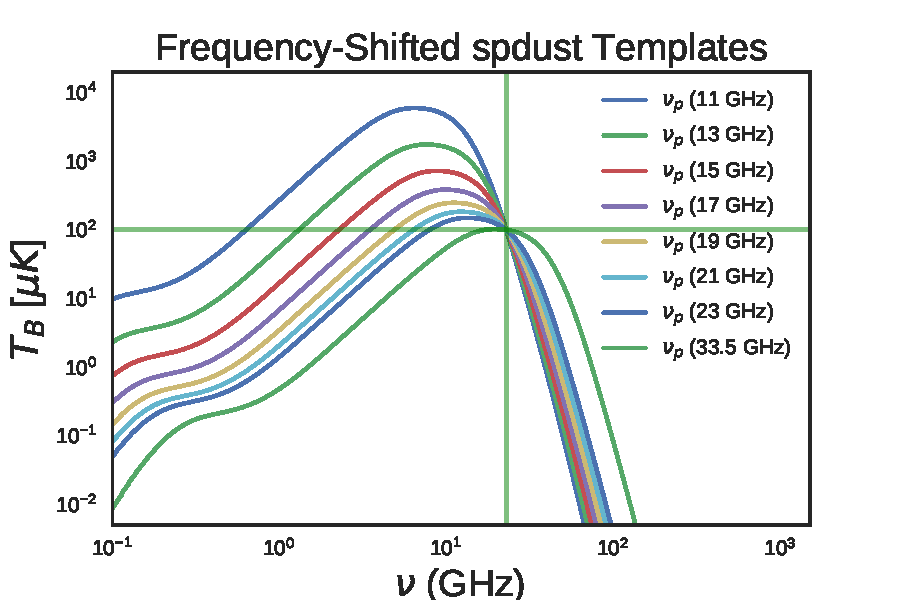
\includegraphics[width=\textwidth]{../Plots/ch_datasources/AME_commander_freqshift_templ.pdf}
                \centering
                \caption{Spdust template spinning dust profiles fitted by PC15X when calculating $AME_{var}$.  The reference frequency, 22.8~GHz is indicated by the vertical green line. Each template has the same $AME_{var}$ amplitude of 100~$\mu$K, indicated by the horizontal green line, plotted to highlight the potential deviation between $AME_{var}$ and the actual peak intensity. }
                \label{fig:AME_commander_freqshift_templ}
              \end{figure}
          PC15X fit the AME by applying a frequency shift and intensity shift parameter to this template. The physical parameters of the {\tt spdust} model itself are not directly varied in PC15X. In any case, the spinning dust model SED shape does not show significant variation from environment to environment \citep{ali-haimoud09}.
         Because of the phenenological approach of the AME fitting method, the PC15X authors themselves suggest caution in deriving conclusions from comparisons with the COMMANDE AME map. However it is the most thorough all-sky component separation currently available, and has not been well analyzed relative to the full wavelength range of available IR all-sky maps. Improving on the COMMANDER AME map will likely require lower frequency constraints (in the red-shaded portion of Fig.~\ref{fig:AME_commander_freqdist}) and/or higher resolution observations of not only the AME itself but the contribution from synchrotron and free-free emisson. This way some of the inherent degeneracies between free-free, synchrotron, thermal dust, and AME parameters may be able to be broken.
          \begin{figure}
               \centering
               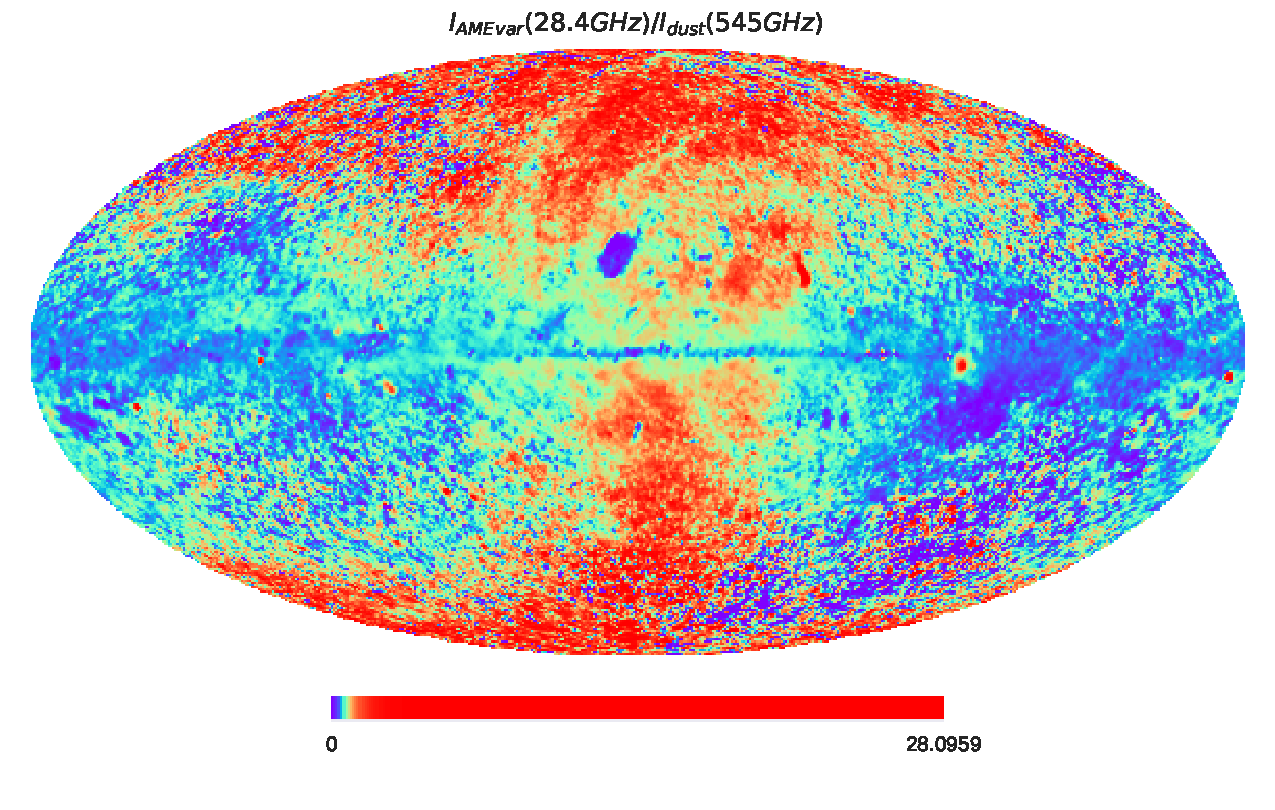
\includegraphics[width=\textwidth]{../Plots/ch_datasources/R_PCAMEtoPCRad.pdf}
               \caption{All-sky map of the ratio of two COMMANDER components- the frequency-varying AME component ($AME_{var}$ divided by the intensity of thermal dust emission at 545~GHz. There are some recognizable AME emission regions, such as $\lambda$~Orionis. Large-scale patches of AME excess are noted to correspond to synchrotron emission \citep{hensley16}}
               \label{fig:R_PCAMEtoPCdust}
           \end{figure}

  \section{All-sky Data Processing}

        The HFI, FIS, and IRIS maps used here are downloaded from their respective online repositories, as all-sky HEALPix\footnote{HEALPix core software is described at \url{http://healpix.sourceforge.net}. The HEALPIx python package {\tt healpy} used in this work is available at: \url{https://github.com/healpy/healpy}} maps \citep{gorski05}. NSIDE~2048 maps. In the case of the IRC maps, we first create HEALPix maps from the 4,857 all-sky survey tiles using the Aladin all-sky data visualization platform \citep{bonnarel00}. NSIDE~2048 implies an average pixel spacing of 1.7$'$. The maps are then degraded to NSIDE~1024 before carrying out a Gaussian-beam smoothing to a 1$^{\circ}$ FWHM. Map smoothing itself is done in spherical harmonic space, before the maps and transformed back to position space. These steps are handled by the smoothing function contained in the {\tt healpy} python package. Following the smoothing process, the maps are degraded once more to NSIDE~256, or 15$'$ pixel-width \footnote{HEALPix pixel scale rebinning carried out with {\tt healpy.ud\_grade}}. The value of each of the larger NSIDE~256 pixels, comes from the mean of its parent NSIDE~1024 pixels. The purpose of this processing is to ensure that all of the maps have the same resolution as the PR2 AME map.

\chapter{Analysis of an interesting AME region: $\lambda$~Orionis}
\label{ch:lori}

 \section{An interesting AME region}
		The $\lambda$~Orionis molecular ring, also known as the Meissa Ring is a massive stucture surrounding the $\lambda$~Orionis O-type star. The ring contains an HII region, ionized by $\lambda$Ori itself and its OB associates \citep{murdin77}. What had been thought of as a star\-forming region of missing molecular gas. At the time \cite{murdin77} even speculated that this could be evidence of an alternate star\-formation pathway, writing: ``Notably we need to know if $\lambda$Ori is an example of a different mode of star formation or [...] simply a case in which the progenitor molecular cloud was exhausted within the last one or two million years.''

    \cite{maddalena86,maddalena87}.  (and references therein) noted a ring of material likely being pushed out by the central, historically well-known $\lambda$~Orionis Association of B-type stars and surrounding HII reigon.

   \subsection{Where does the ring come from?}
    \cite{cunha96} argued that the ring may have resulted from a supernova explosion, further speculating that $\lambda$Ori may have been a companion of the progenitor. $\lambda$~Orionis is a known binary system, however its current companion is the a B-type star. \citep{murdin77}
  .
     The central region is heated by the $\lambda$~Orionis star itself, and the Orion~OB association it belongs to \citep{ochsendorf15}. The region is known to host several young stellar and protostellar objects \citep{koenig15}.

    At approx. 10$^{\circ}$ wide, we can see the outline of the structure even in the low (1$^{\circ}$ FWHM) resolution PCAME map. The ring shape itself is thought to originate from a supernova, or perhaps combined effects of the entire star formation history of the $\lambda$~Orionis Association, including the formation of its surrounding HII region \citep{aran09}.

  \subsection{A well-studied region}
    Although the $\lambda$~Orionis region has been a popular target for study since approximately the 1980s. \cite{duerr82} wrote of the relative lack of work on the overall region: ``Surprisingly, this interesting complex has been little studied''. While this seems surprising given the numbe of works on the region in the literature now, it is really the advent of all-sky missions that have driven more recent interest.  The large angular size is such that all-sky surveys were a natural boon for study of such extended structures. WISE especially was a huge source of insight \citep{koenig15}. More recently, \cite{planck15XXV} strongly highlighted the region as a strong candidate for further AME investigation.

\section{Investigative approach}
  We have carried out an initial comparison of the AME of this region with its mid to far-IR dust emission. The region is shown in Fig.~\ref{fig:orionis-akari9} as it appears in 1$^{\circ}$-smoothed A9 data.
      \begin{figure}
        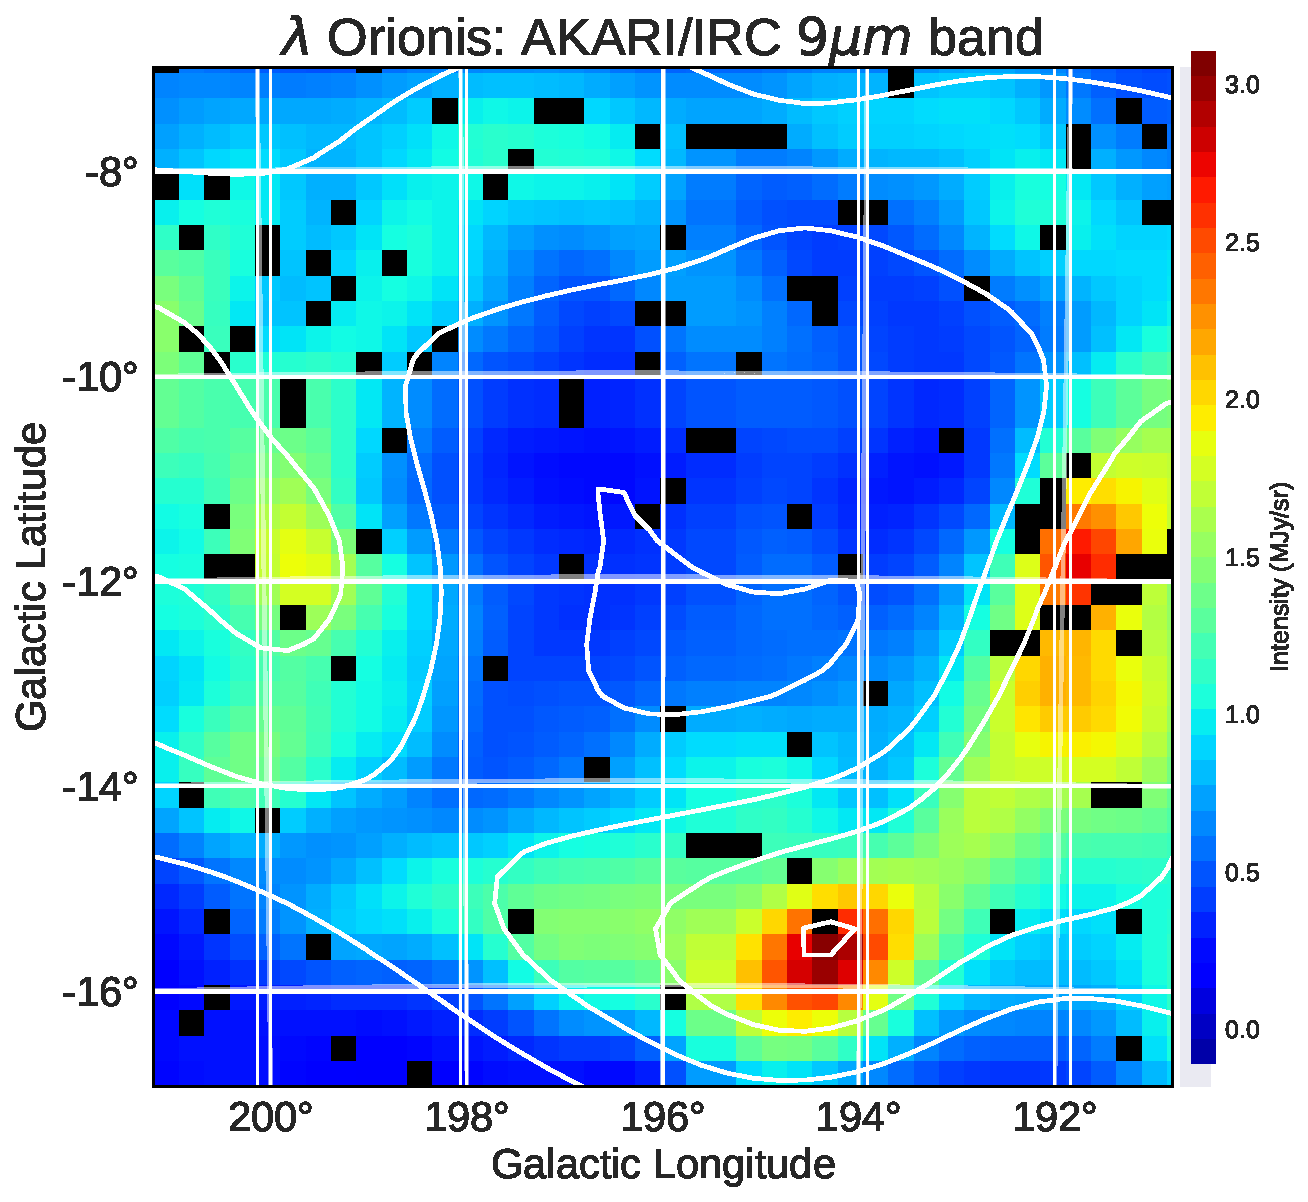
\includegraphics[width=\textwidth]{../Plots/LOri_akari9_AMEcont_1dres.pdf}
        \centering
        \caption{$\lambda$~Orionis as it appears in the AKARI 9~$\mu$m data. Contours indicate the AME, as given by the Planck PR2 AME map. The image is smoothed to a 1$^{\circ}$ PSF (much larger than the original 10 arcsec map). The $\lambda$~Orionis star itself is approximately located at the center of the image.}
        \label{fig:orionis-akari9}
      \end{figure}
   The ring structure itself indicates excess microwave emission attributed to AME, from the dominant variable frequency component $AME_{var}$ (see Ch.~\ref{ch:datasources}). The central region is dominated by free-free emission \citep{aran09, koenig15}. Free-free emisison coming from the Hii phase surrounding the $\lambda$~Orionis association dominates the region's morphology in LFI images. \citep{planck15XXV}. Taking the hint from \cite{planck15XXV} that this may be among the more reliably component separated regions, we evaluate if there is any preferential relationship between any parameter of dust emission and the AME. Fig.~\ref{fig:LOri_halpha_AMEvarContours} shows the expected distribution of free-free emission in the region, assuming that $H\alpha$ line emission is a tracer of microwave free-free. This indicates that free-free is strong within the central region, where radiation fields are more intense, and AME is minimal. The strongest AME follows the ring-shaped morphology outside the central bubble of free-free emission.
     \begin{figure}
       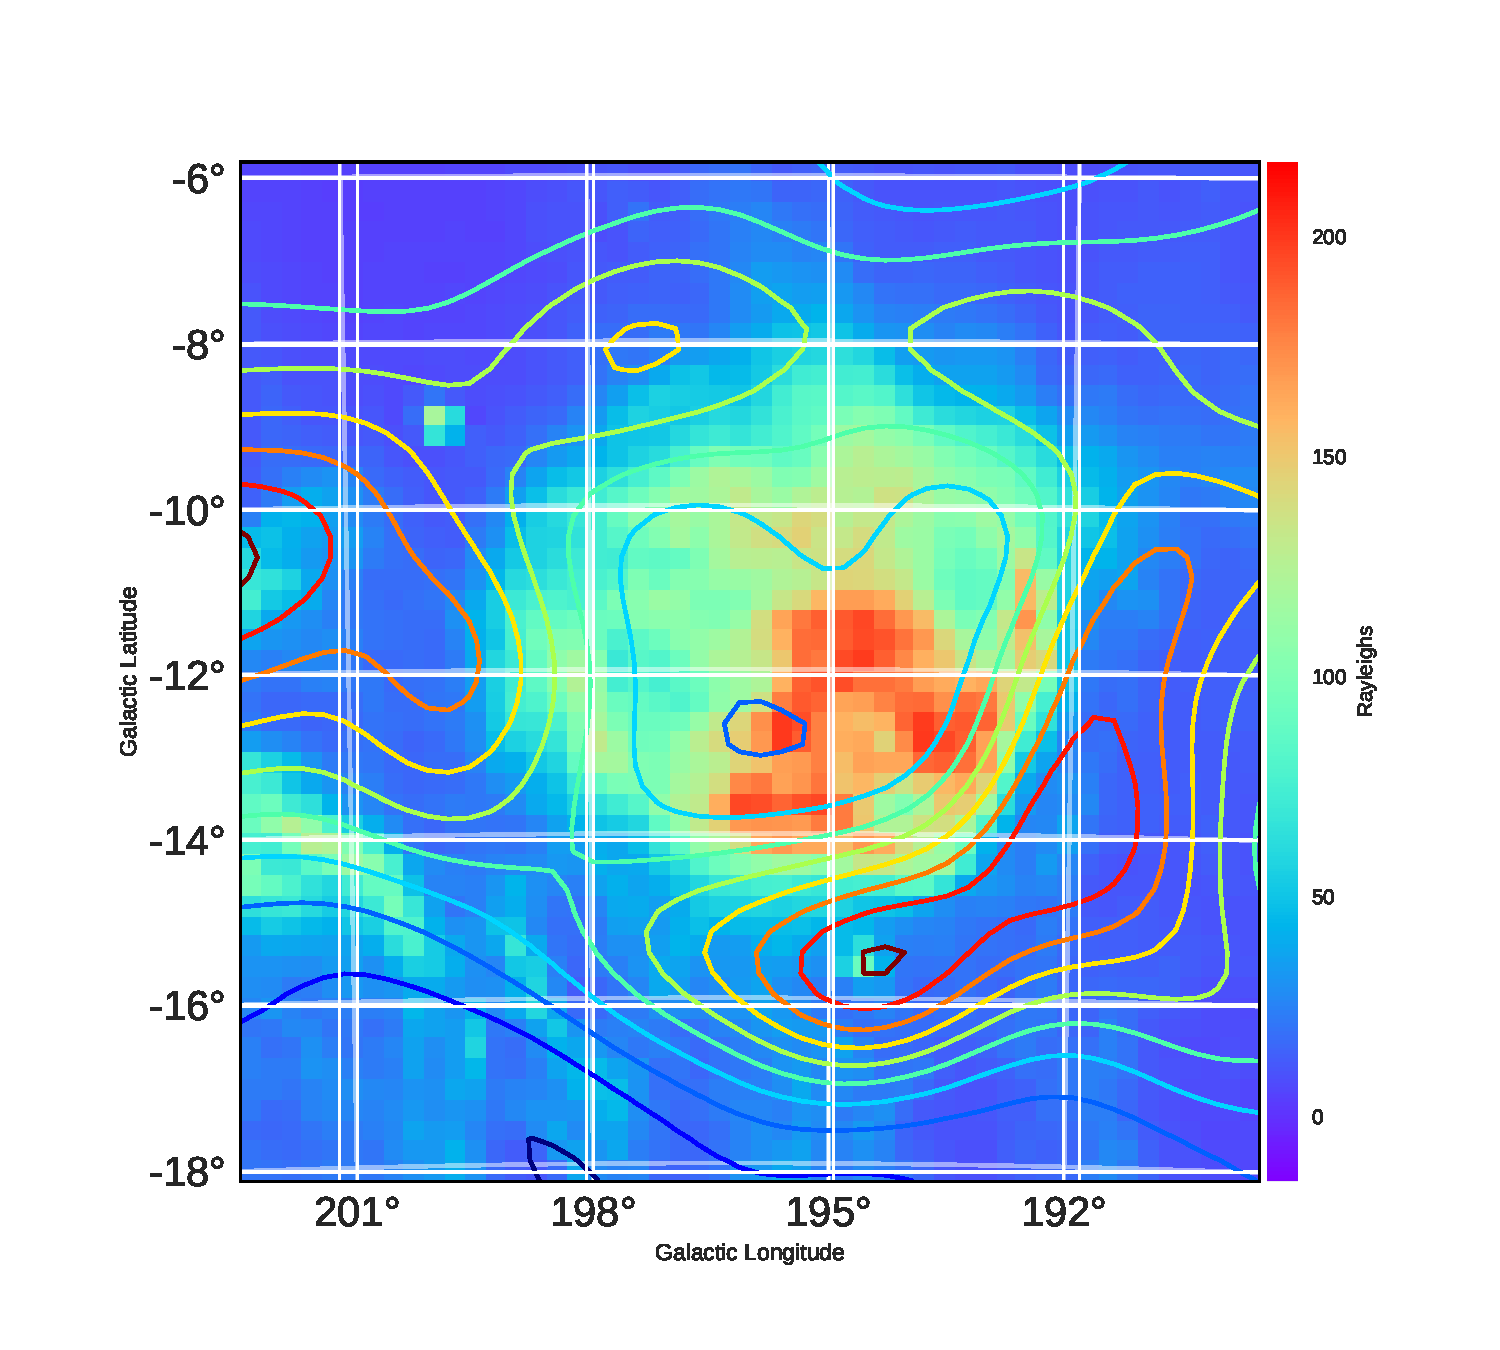
\includegraphics[width=\textwidth]{../Plots/ch_lori/LOri_halpha_AMEvarContours.pdf}
       \centering
       \caption{$\lambda$~Orionis as it appears in H-alpha emission by \cite{finkbeiner03}. Contours indicate AME emission, from the variable frequency component. The colorbar indicates $H\alpha$ emission in Rayleighs. The field of view is slightly larger than that used for the final processed IR comparison (Fig.~\ref{fig:lori_processed_all}). }
       \label{fig:LOri_halpha_AMEvarContours}
     \end{figure}

	\section{Data preparation}
    \label{sec:dataprocessing}
		As indicated in Ch.~\ref{ch:datasources}, we use 12 photometric all-sky maps. For the IRC data (A9 and A18), we produce mosiacs of $\lambda$~Orionis from the individual tiles provided in the internal all-sky archive.
      \footnote{IRC all-sky data is still in the proprietary phase at the time of this writing, but should be public by April 2018.}
       For the other sources, HEALPix all-sky maps are available publicly, at sufficient resolution relative to their native resolutions\footnote{Planck data was retreived from the NASA IPAC online archive at \url{http://irsa.ipac.caltech.edu/data/Planck/release_2/all-sky-maps/}}. \footnote{AKARI/FIS data }\footnote{IRAS/IRIS data }

		\subsection{Extraction from HEALPix maps}
		  For the data obtained via HEALPix maps, we employ the {\tt healpix2wcs} functionality provided in the {\tt gnomdrizz} python package\footnote{Available at \url{http://cade.irap.omp.eu/dokuwiki/doku.php?id=software}}\footnote{``drizzlib'' 1.2.2 and earlier were not able to correctly access HEALPix files with multiple fields/columns. See appendix for our recommended workaround.} A9 and A18 images are produced by regridding the images with the {\tt Montage} software by NASA/IPAC. Figs.~\ref{fig:lori_A9_mosaic_smooth} and~\ref{fig:lori_A18_mosaic_smooth} show high resolution mosaics of the A9 and A18 data before processing. All of the images for all of the bands are based on a common FITS header which has a pixel grid spacing equal to the average pixel width in the NSIDE 256 HEALPix scheme.

      \subsection{Point-source and artifact masking}

        \paragraph{Missing stripes}
          The AKARI all-sky survey suffers from a few missing stripe errors throughout the IRC and FIS maps \citep{ishihara10, doi15}. This is a more serious issue for FIS. They can generally be characterized as a competition for integration time beteen the all-sky observing mode, and pointed observations during AKARI's crygoenic phase. Unfortunately for the present work, some of these stripes pass directly through the $\lambda$~Orionis region. Figs.~\ref{fig:LOri_FIS_color},~\ref{fig:lori_A9_mosaic_smooth} and ~\ref{fig:lori_A18_mosaic_smooth} display the data at near-native resolution, demonstrating where these patterns occur. Additionally there are some saturated pixels in both IRC and FIS data.
            \begin{figure}
              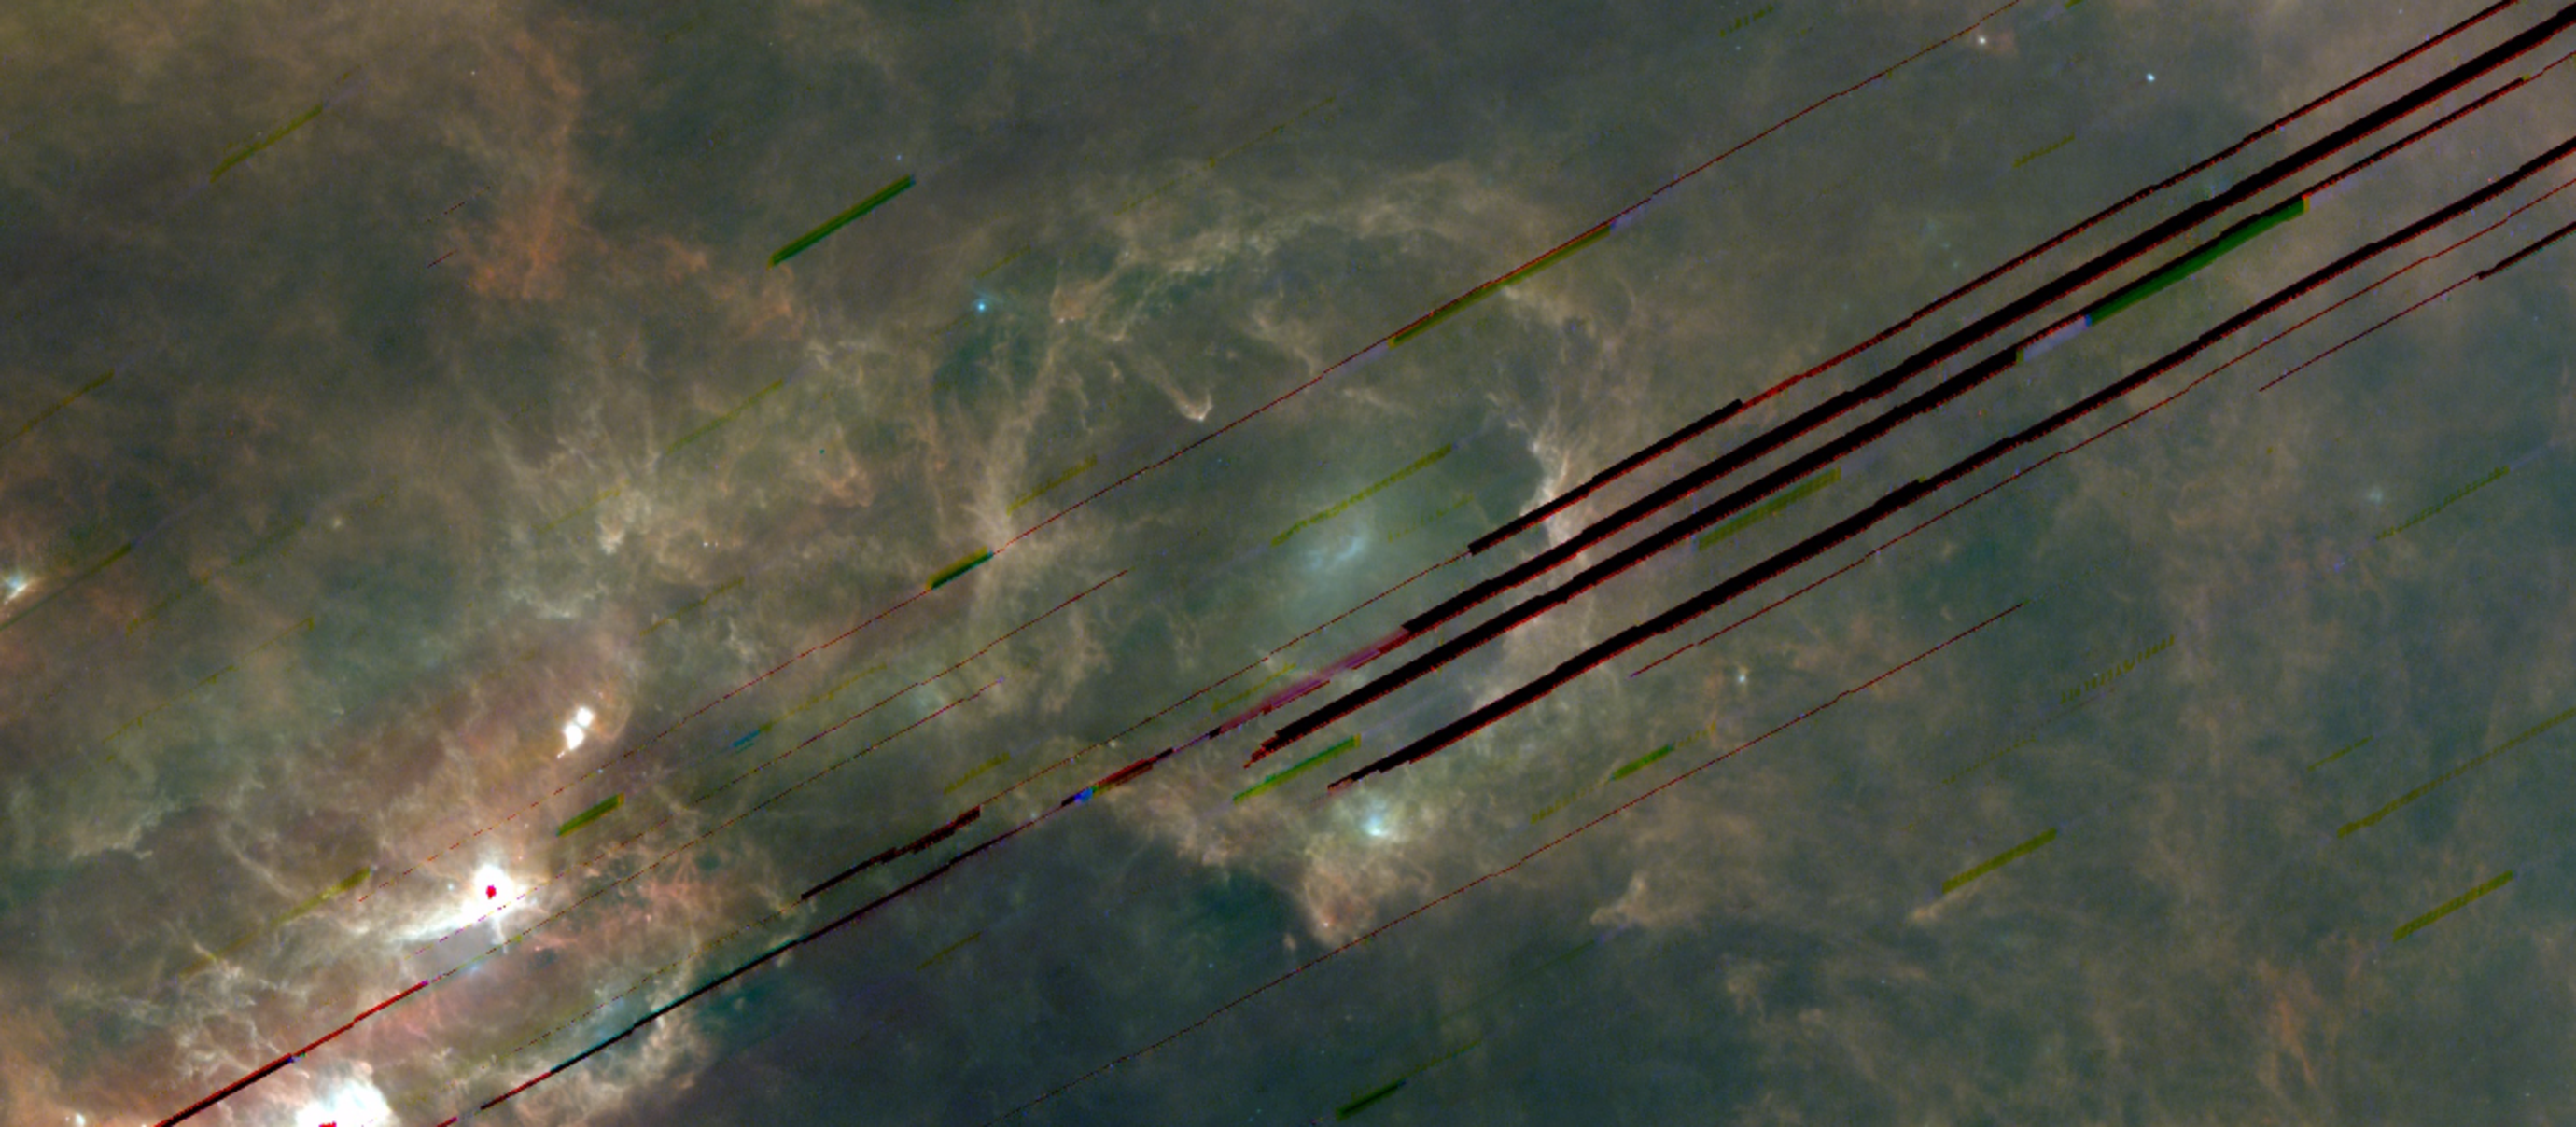
\includegraphics[width=\textwidth]{../Plots/ch_lori/lori_fis_rgb.pdf}
              \centering
              \caption{The $\lambda$~Orionis region and its surroundings in AKARI FIS data, where A65 is blue, A90 is green, and A140 is red. The missing stripe patterns are visible, and affect all 3 bands shown here as well as the A160 data. }
              \label{fig:LOri_FIS_color}
            \end{figure}
            \begin{figure}
              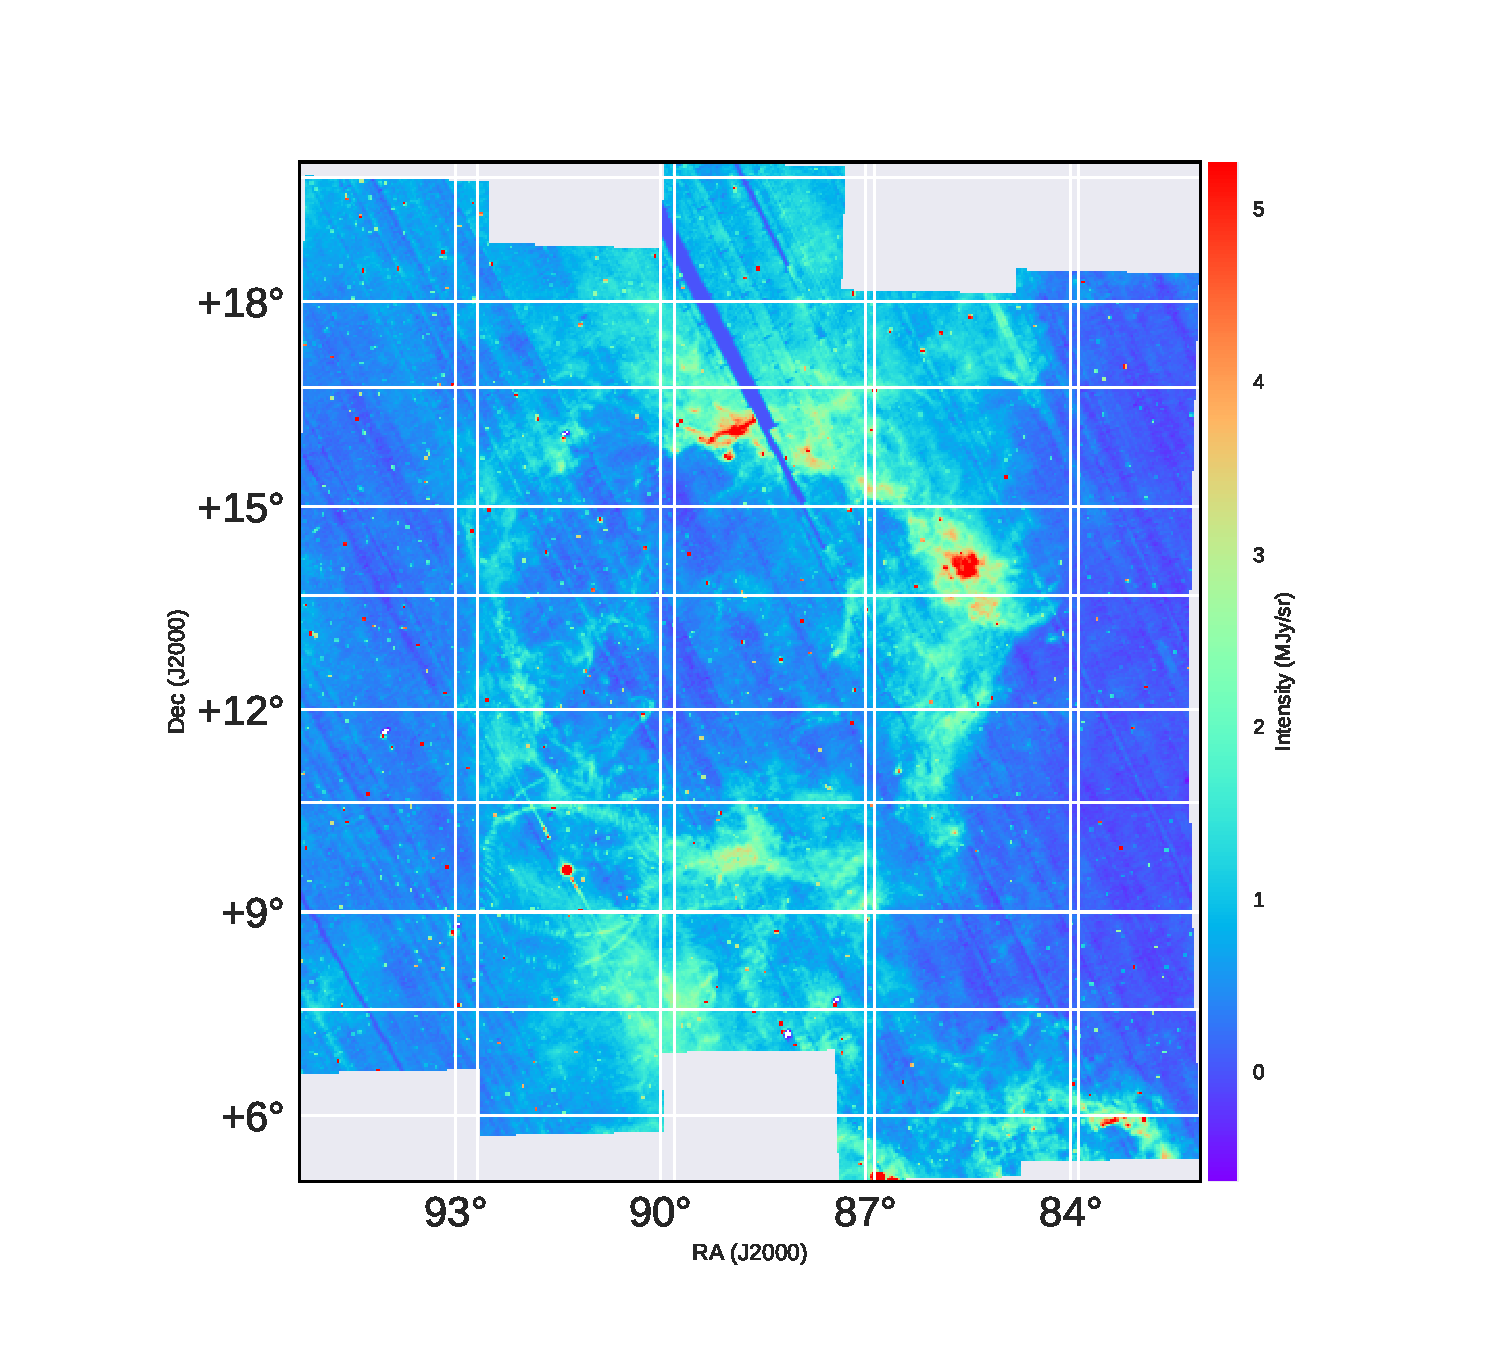
\includegraphics[width=\textwidth,trim={2.5cm 2cm 3.0cm 2cm},clip]{../Plots/ch_lori/lori_A9_mosaic_smooth.pdf}
              \centering
              \caption{The $\lambda$~Orionis region in the A9 band at near-native resolution. This is a mosiac created from the 3x3 degree all-sky survey tiles by Ishirara et al. (in prep.) Missing stripes are less of a problem than with the A18 band (Fig.~\ref{fig:lori_A18_mosaic_smooth}), but point sources are more pronounced. Betelgeuse, in the lower left of the image, is bright enough in this band to produce a ring-shaped artifact. }
              \label{fig:lori_A9_mosaic_smooth}
            \end{figure}
            \begin{figure}
              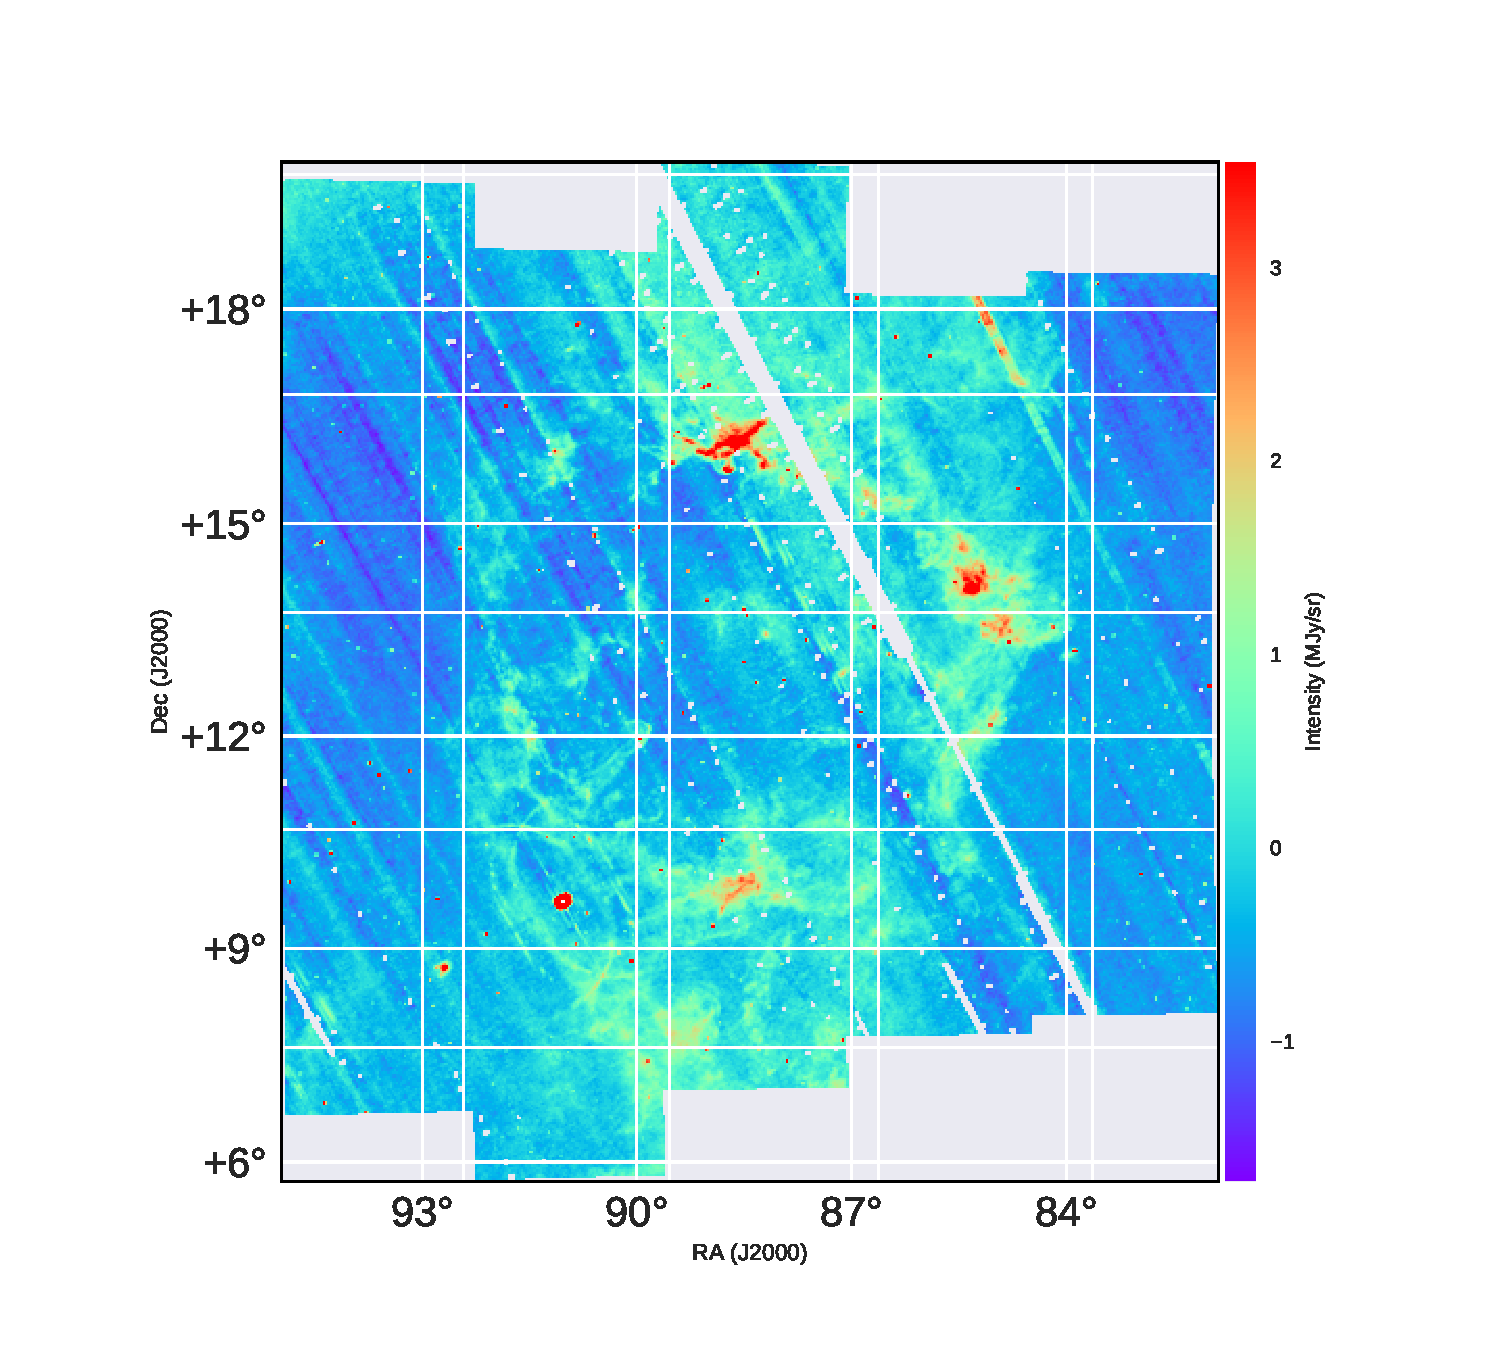
\includegraphics[width=\textwidth,trim={2.5cm 2cm 3.0cm 2cm},clip]{../Plots/ch_lori/lori_A18_mosaic_smooth.pdf}
              \centering
              \caption{The $\lambda$~Orionis region in the A18 band at near-native resolution, demonstrating the regions affected by missing stripe errors, but less affected by point-sources than A9 (Fig.~\ref{fig:lori_A9_mosaic_smooth}). }
              \label{fig:lori_A18_mosaic_smooth}
            \end{figure}

        \paragraph{Point sources}
          A caveat that comes with added ionized PAH feature coverage of the A9 band, is that the shorter central wavelength placement allows more contamination from point sources. We identify point sources with a moving-window approach provided in the astropy Python package, flagging pixels which have higher than 5$\sigma$ intensity among the surrounding 100 pixel window. We then place a mask at the center of the flagged point-sources. The masks are propogated through the regridding step, such that the low-resolution pixels having more than 50\% of their area masked in the high resolution tiles, also become masked. Such pixels appear black in Fig.~\ref{fig:orionis-akari9}. The same process is applied to the A18 data. For other maps, which we extract from HEALPix data, we first regrid from HEALPix to rectangular grids, and then apply the point-source search and masking as above. For the I12 and I25 images, the rejected pixels were fewer than with A9, but positions overlapped with those already masked in A9. For bands longer than I25, this process did not result in rejected pixels. For the D12 and D25 bands, which are natively at a much lower resolution than AKARI or IRAS, point-sources present more of a challenge. For these images, we visually inspect and mask 3 regions with bright point source contamination consistent with the DIRBE beamsize and with point-sources identified in IRAS and IRC images. Pixel positions masked in any single image, are masked in all of the images before the finaly analysis.


        \subsection{PSF Smoothing}
          We smooth the pixels in the spatial domain, to have a 1$^{\circ}$ FWHM PSF, in order to have a resolution approximating that of the PC AME data.
          The smoothing process relies on the {\tt convolution} module provided in the {\tt astropy} package. We assume simple circular gaussian kernel for the smoothing process. While they may be asymmetries in the effective beam shapes of the IR bands used, the target resolution of the AME data is large enough relative to the native resolution of the input IR data (especially A9 and A18, see Fig.~\ref{tab:data}) as to render the beam shapes and positional variations negligible. Finally, we mask pixels along the edge of the FOV where the convolution process produces artifacts.

      \subsection{Background subtraction}
         We estimate an average, flat background level for this region. The background level is determined the mean of pixels in an `OFF` zone. The final images are shown in Fig.~\ref{fig:lori_processed_all}, with the full mask applied (masked pixels are indicated in white), and with the OFF zone indicated by the red rectangle on each frame.
            \begin{figure}
              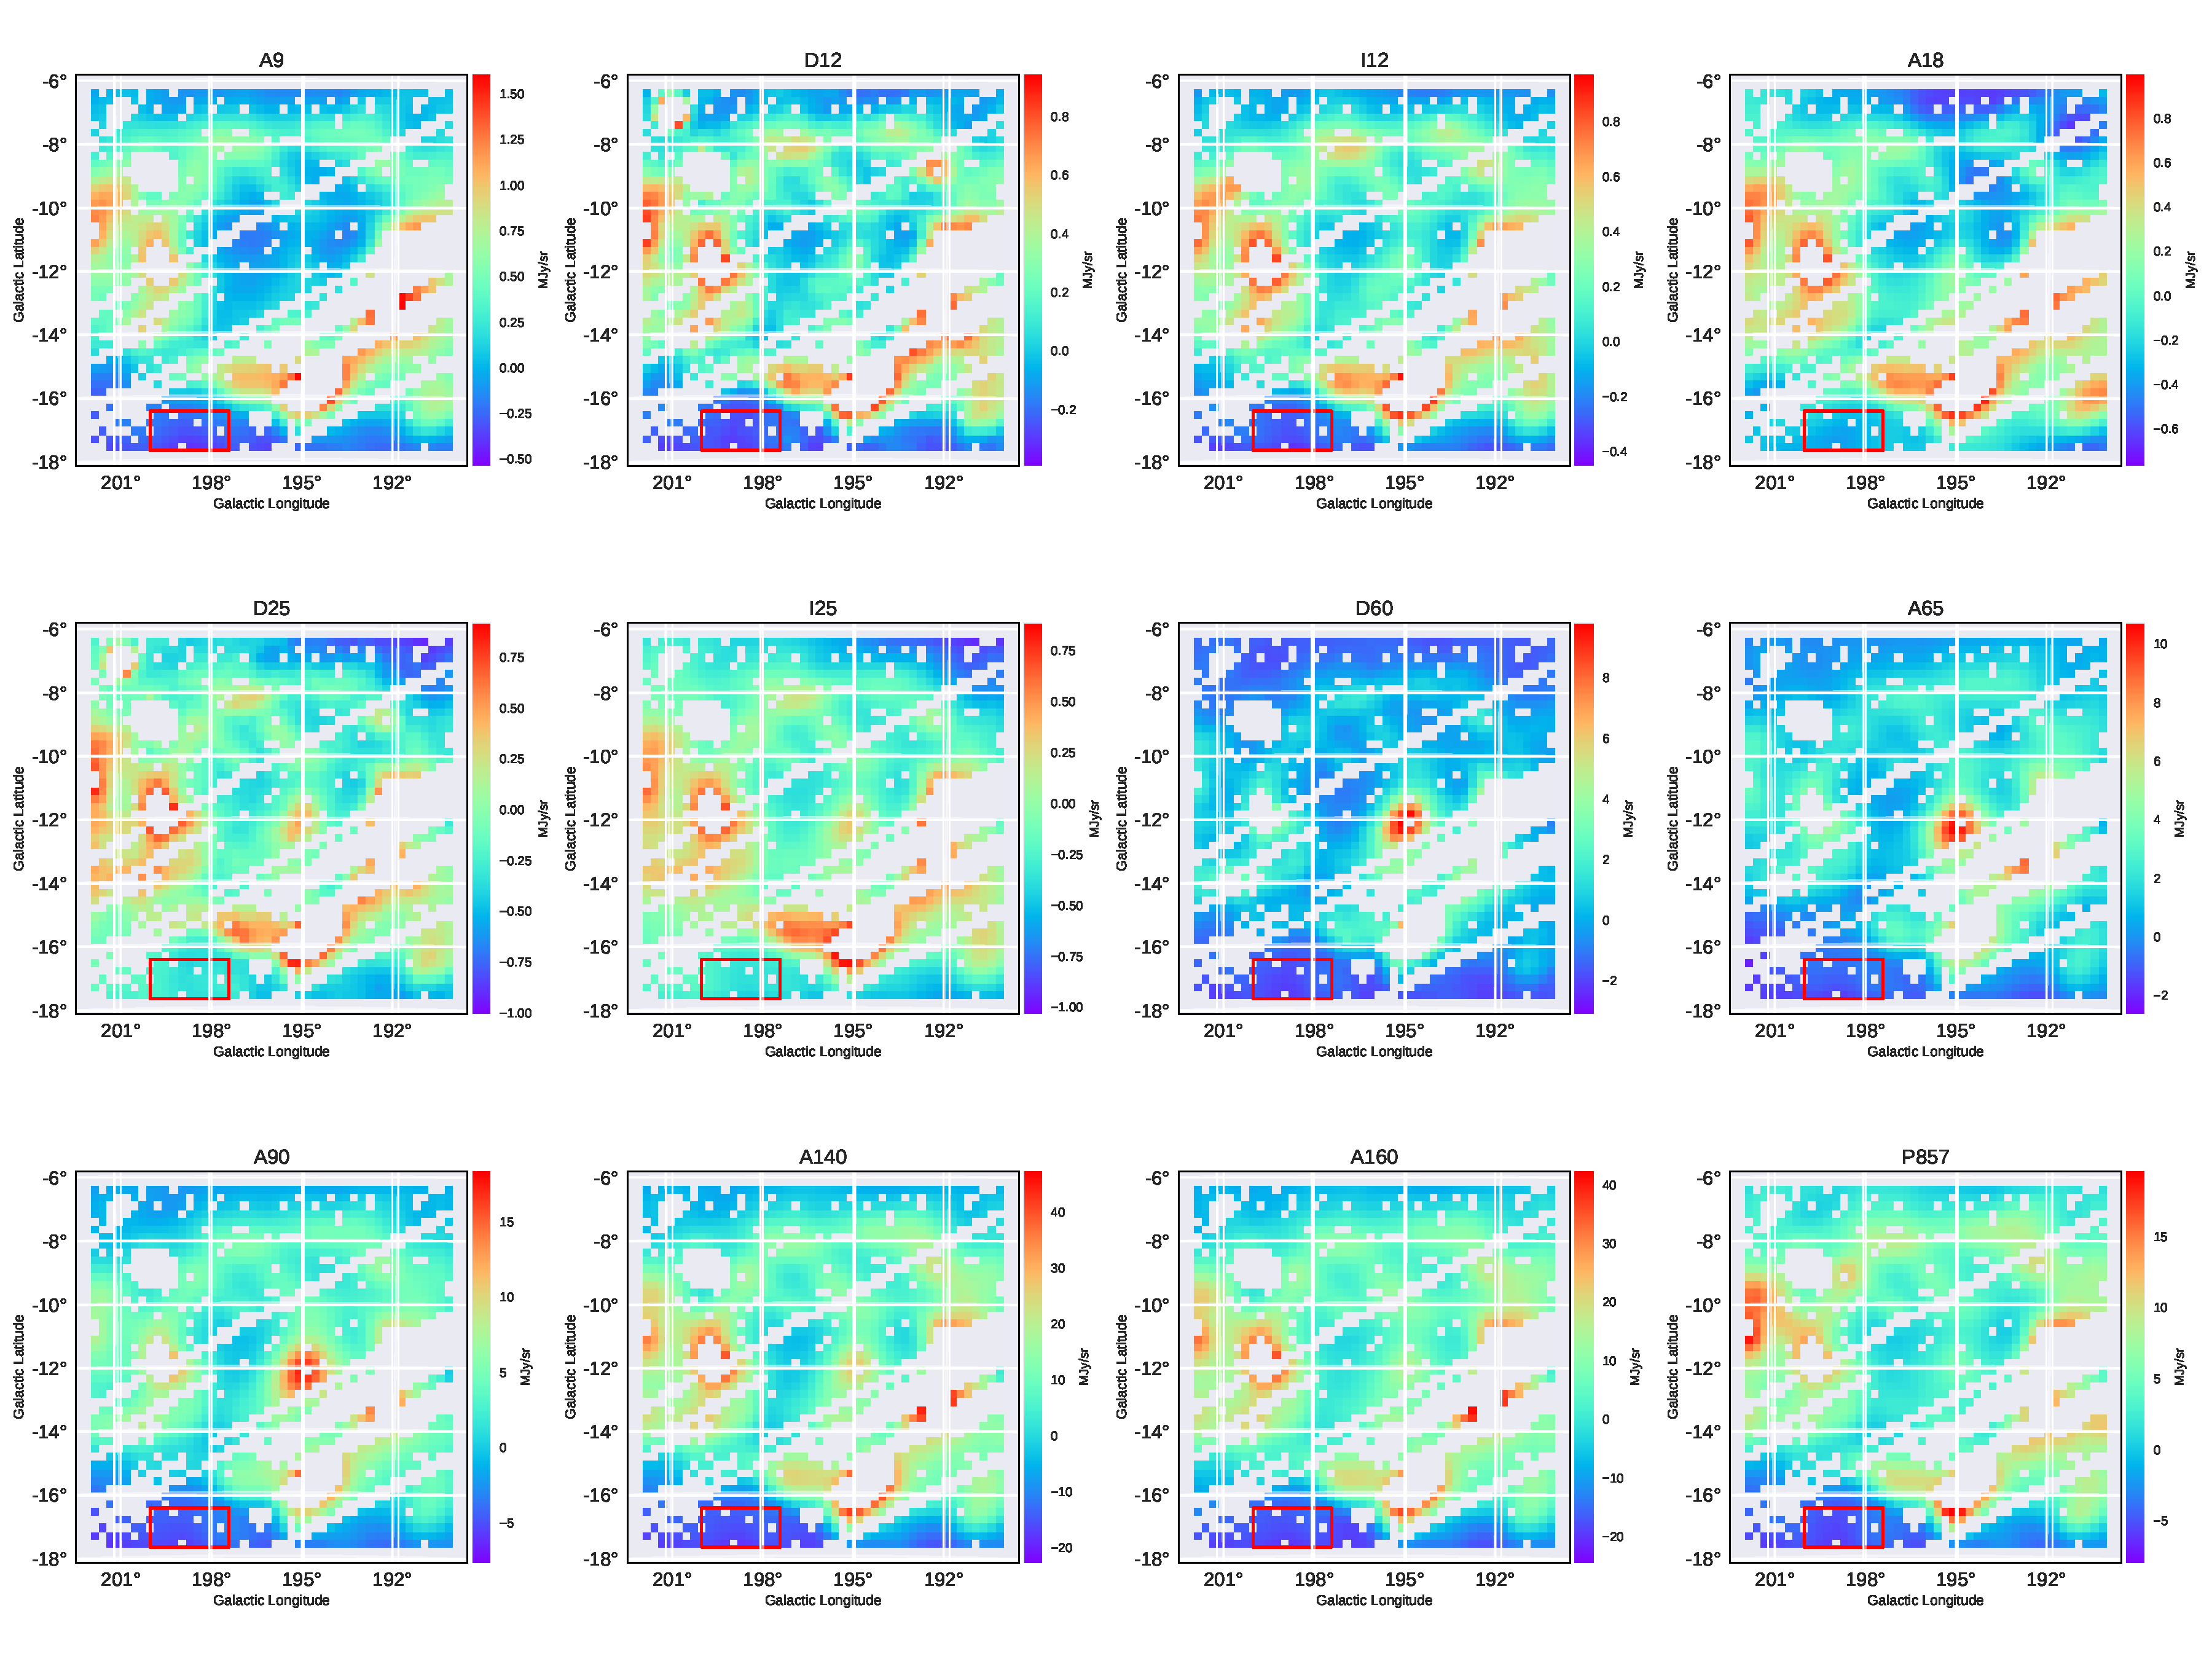
\includegraphics[width=\textwidth,trim={5cm 5cm 3.5cm 5cm},clip]{../Plots/ch_lori/lori_processed_grid.pdf}
              \centering
              \caption{Processed data at each wavelgnth for $\lambda$~Orionis. A flat background has been subtracted from each frame based on the mean of pixels within the red rectangle. The pixel width is 0.25$^{\circ}$, with the data PSF smoothed to 1$^{\circ}$ spatial resolution. Masked pixels (point sources, stripe errors, convolution artifacts) are shown as white. The frames share the same FOV and GAL-TAN projection. Colorbars indicate the intensity in MJy/sr.}
              \label{fig:lori_processed_all}
            \end{figure}
          We do not expect simple band-by-band intensity correlation tests with the AME to be sensitive to background and foreground emission along the line of sight towards the $\lambda$~Orionis region. However analyses such as dust SED fitting, to determine the relative abundances of different dust components, may be effected by the background level. The general morphology as seen in the high resolution AKARI data (Figs.~\ref{fig:LOri_FIS_color},~\ref{fig:lori_A9_mosaic_smooth} and ~\ref{fig:lori_A18_mosaic_smooth}) remains well pronounced in the final, low resolution images.

	\section{Multi-wavelength characterization}
    The correlation matrix results corresponding to data shown in Fig.~\ref{fig:lori_processed_all}, are shown in Fig.~\ref{fig:orionis-corr-matrix}.
      \begin{figure}
        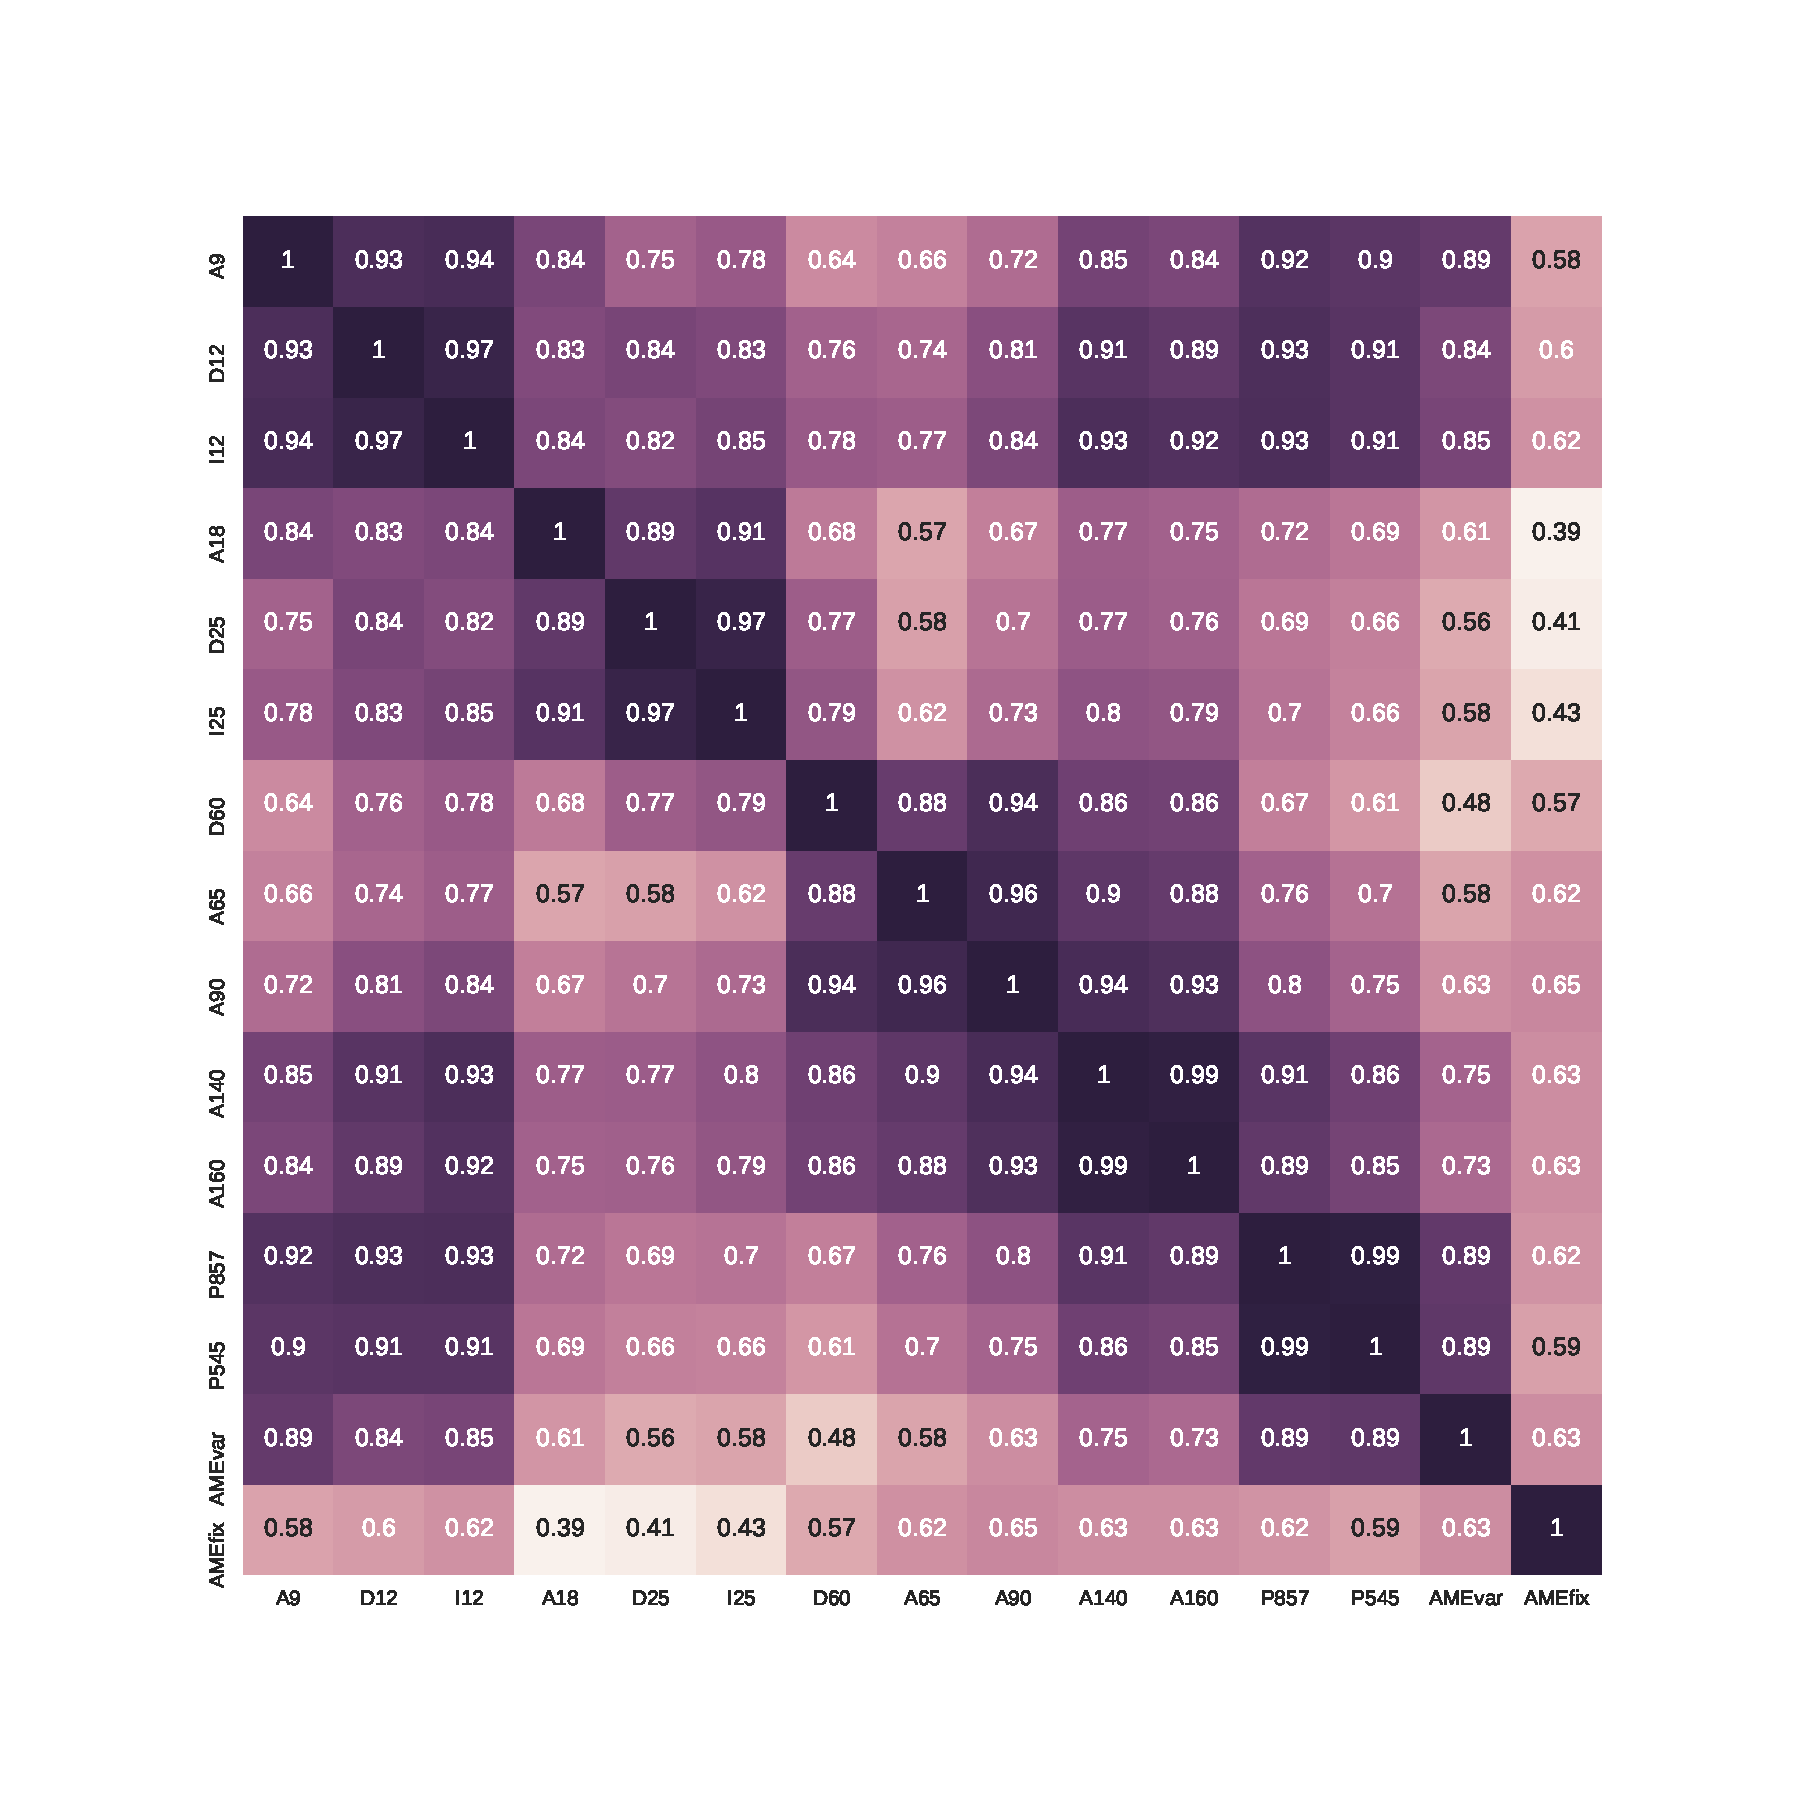
\includegraphics[width=\textwidth]{../Plots/ch_lori/Lori_corrmatrix_I.pdf}
        \centering
        \caption{$r_{s}$ correlation matrix for all of the data used in the $\lambda$~Orionis analysis, similar to that presented for the Planck Commander component maps in Fig.~\ref{fig:PCCS_corrmatrix}. The shade and annotation for each cell indicates the $r_{s}$ score, where $r_{s}$ of 1 indicates a monotonically increasing relationship for a given pair of images. The two AME components, as described in Ch.~\ref{ch:datasources}, are listed separately: $AME_{var}$ for the frequency-varying component, and $AME_{fix}$ for the constant frequency component.}
        \label{fig:orionis-corr-matrix}
      \end{figure}
     This immediately confirms a correlation between the IR and AME, however this was readily visibly from the spatial morphology of the region. Interestingly though, the correlation strengths with $AME_{var}$ show a pattern from short to long wavelengths: A9, P857, and P545 show the strongest correlations, with the correlation weaking from A18 to A90, and again strengthening at longer wavelengths. The fixed peak frequency $AME_{fix}$, which is the much fainter component, shows the strongest correlation with A90- though all of the IR correlations relative to $AME_{fix}$ are weaker than those for $AME_{var}$. The overall pattern is for bands dominated by PAH emission (as discussed in Ch.~\ref{ch:datasources}), and those which trace Rayleigh-Jeans thermal dust emission are equally good predictors of the AME. Bands dominated by a mixture of VSGs, and warm dust emission, show a weaker correlation. For the next stages of analysis, we will consider only the dominant component $AME_{var}$. We found that combining the components does affect the results here.

     Comparing the images in Fig.~\ref{fig:lori_processed_all}, most of the variation in the correlation scores appears to come from the central region of $\lambda$~Orionis. Because of the known heating present within the ring, from the $\lambda$~Orionis association, and given the brightening of bands between A18 and A90, this variation appears to be due to a temperature increase.
    \subsection{Bootstrap analysis}
        To assess the robustness of the correlation scores, we employ the Bootstrap re-sampling approach, first introduced by \cite{efron79} (see \cite{feigelson13} for an updated description within an astronomical context). This involves creating random re-sampled sets of the data. We use the 'with replacement' approach, meaning that a data point may be selected multiple times in a single re-sampling iteration. The size of the re-sampled set is the same is the input set size. For each random set we run a correlation test, resulting in a distribution of correlation coefficients. This allows us to estimate error bars for the correlation scores, and effectively de-weight outliers within each sample.
        We carry out bootstrap correlation tests for each IR band's intensity vs. $AME_{var}$ . The data are resampled 10,000 times for each correlation test, a sufficient resampling given the unmasked pixel count of \textasciitilde{}1400 pixels, and considering that the effective beams are somewhat undersampled. This is repeated for both $r_{s}$ and $r_{p}$ based tests, in order to assess variations in degree of linearity among the various IR:AME trends. The distributions of the boostrap resamplings are shown in in Fig.~\ref{fig:bootstrap_vs_AME}.
            \begin{figure}
              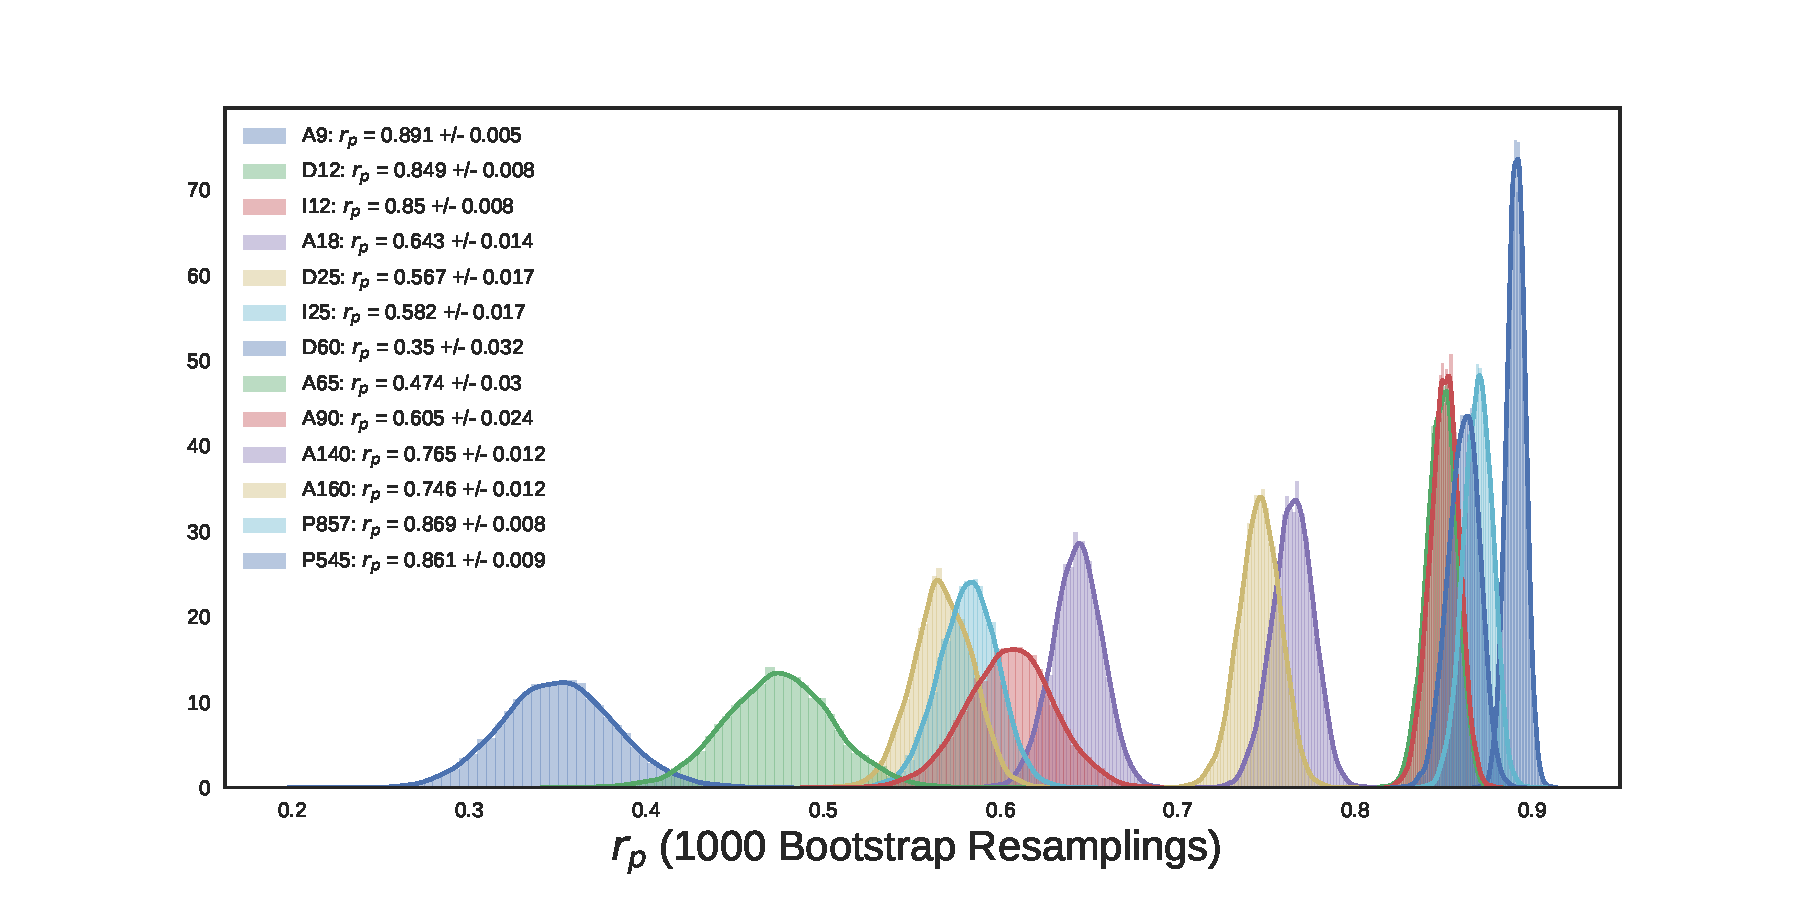
\includegraphics[width=\textwidth,trim={3cm 0.25cm 2.5cm 1cm},clip]{../Plots/ch_lori/bootstrap_vs_AME_pearson_i10000.pdf}
              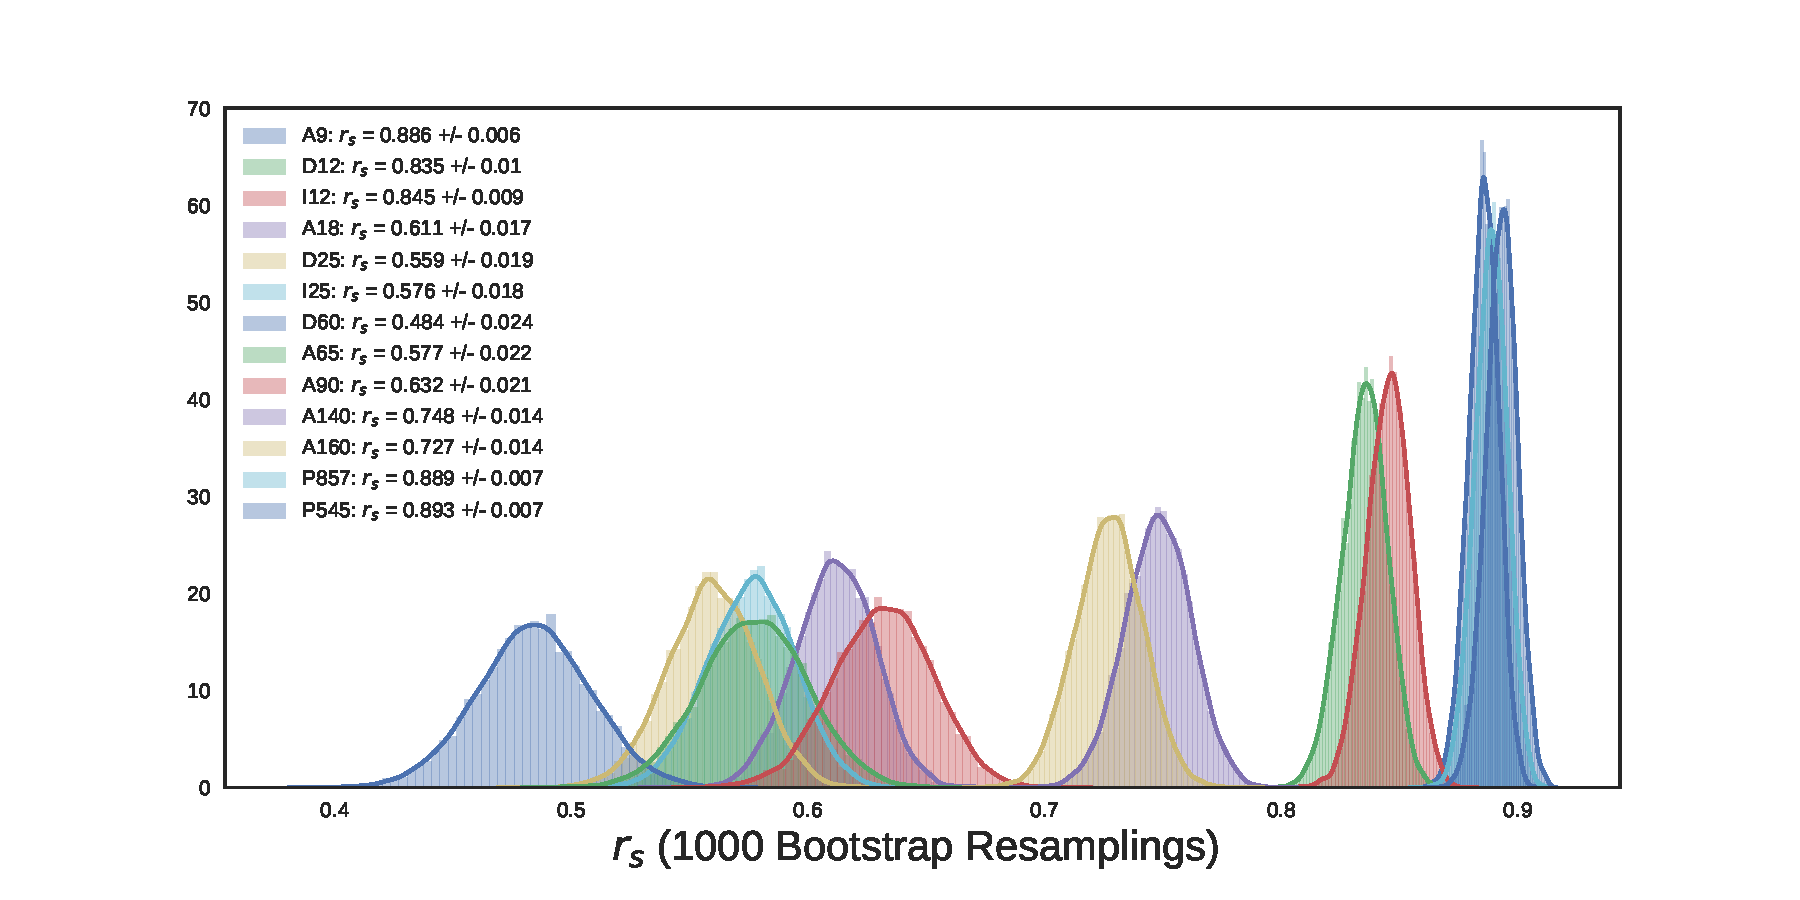
\includegraphics[width=\textwidth,trim={3cm 0.25cm 2.5cm 1cm},clip]{../Plots/ch_lori/bootstrap_vs_AME_spearman_i10000.pdf}
              \centering
              \caption{Re-sampled (Bootstrap) correlation tests for IR emission in $\lambda$~Orionis vs. AME, for both $r_{p}$ (upper) and $r_{s}$ (lower) cases. Each band's $r$ distribution is shown in a different color (the same color scheme for both plots). The width of the distribution indicates the error for the given data in the correlation coefficient. The mean and standard deviation of the scores are given in the legend of each plot. The plot ranges only show positive values, since no negative scores were produced. }
              \label{fig:bootstrap_vs_AME}
            \end{figure}
        For both test cases, the best correlations are the longest and shortest wavelength bands, consistent with the straight-forward $r_{s}$ scores shown in Fig.~\ref{fig:orionis-corr-matrix}. In the $r_{p}$ case, the strongest correlation is the A9 band vs the AME.
        \section{Comparison with SED Fitting}
          We performed a full dust SED fitting on the $\lambda$~Orionis photometry, according to the dust model by \cite{galliano11} (to be thoroughly introduced in Galliano, et al., in prep.)  We used a mixture of silicate and carbonaceous dust, silicate dust, the two dominant categories of interstellar dust as described in Ch.~\ref{ch:intro}. However, instead of the graphite-based carbon dust invoked by the canonical \cite{draine07} model (DL07), we assume amorphous carbon. This choice is an attempt to account for the ``sub-mm excess'' of dust emission, reported by \cite{israel10, bot10}, in the Large Megallanic Cloud (LMC). The increased emissivity of amorphous carbon (a factor of 2-3 more than DL07) allows a better fit to Herschel observations of the LMC \citep{galliano11}, and Planck observations of the Milky Way \citep{planckIntXXIX16}. We assume that the radiation field heating this dust mixture is the Galactic ISRF \citep{mathis83}, scaled by a factor $U$.
        %   We also assume, following \cite{dale01}, that the dust is exposed to a distribution of starlight intensity, distributed as:
        %       \begin{equation}
        %          \label{eq:U}
        %            dM_{dust}\propto{} U^{-\alpha}dU
        %       \end{equation}
        %   between $U_{min}$ and $U_{max}$, where $U_{min}$, $U_{max}$ and $\alpha{}$ are free parameters.
          We utilize both the Bayesian dust SED fitting approach by Galliano (in prep.), and a least-squares analysis. The SED fitting accounts for estimates of the respective calibration uncertainties, and the spectral response curves (Fig.~\ref{fig:Filter_coverage_example_full}). As outputs, metrics of the total dust mass $M_{dust}$, PAH mass $M_{PAH}$, ionized PAH mass $M_{PAH+}$, and ISRF intensity $U$ are produced. We only carry out the fitting for unmasked pixels. We are primarily interested in which of the corrleations $M_{dust}$ vs. $I_{AME}$ or $M_{PAH}$ vs. $I_{AME}$ is stronger.
          Two sample fitting results are shown in Figs.~\ref{fig:fred_LOri_notes_Oct2017_fig1a}, and~\ref{fig:fred_LOri_notes_Oct2017_fig1b}.
              \begin{figure}
                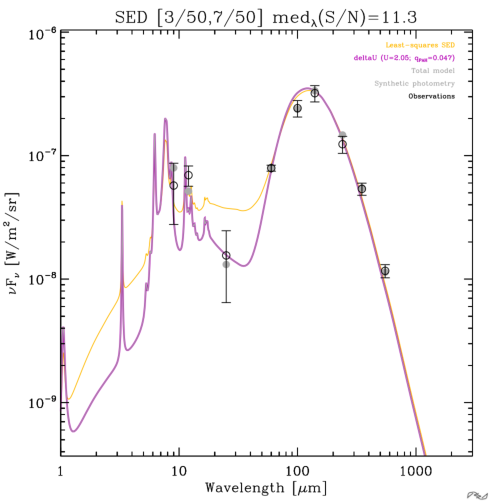
\includegraphics[width=\textwidth]{../Plots/ch_lori/fred_LOri_notes_Oct2017_fig1a.pdf}
                \centering
                \caption{Observed (black circles and errors) and synthetic photometry (gray dots) SED of a pixel within $\lambda$~Orionis, along with the dust SED model fit results. Two SED fits are shown: on for the Bayesian fitting (magenta), and another showing the standard least-squares result for comparison (yellow). The fitted ISRF strength $U$, and fraction of mass in PAHs, $q_{PAH}$ are also given.}
                \label{fig:fred_LOri_notes_Oct2017_fig1a}
              \end{figure}
              \begin{figure}
                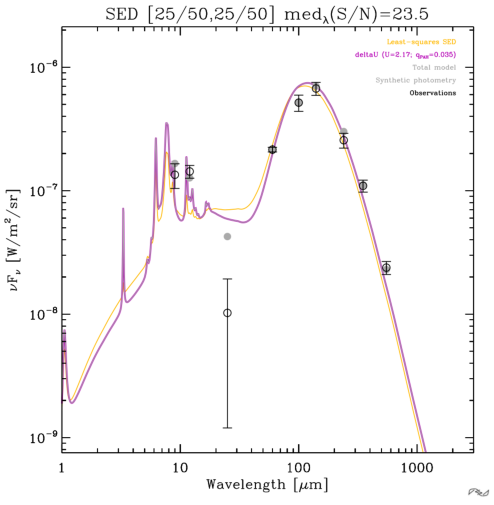
\includegraphics[width=\textwidth]{../Plots/ch_lori/fred_LOri_notes_Oct2017_fig1b.pdf}
                \centering
                \caption{The same as Fig.~\ref{fig:fred_LOri_notes_Oct2017_fig1a}, but for a different pixel position. Corresponds to galactic coordinates...}
                \label{fig:fred_LOri_notes_Oct2017_fig1b}
              \end{figure}
           Performing such fits for all of the pixels, we are able to see how $I_{AME}$ varies with the bulk dust physical characteristics of the region. Fig.~\ref{fig:fred_LOri_notes_Oct2017_fig2a} shows the fitted dust mass per pixel, relative to the AME intensity.
                \begin{figure}
                 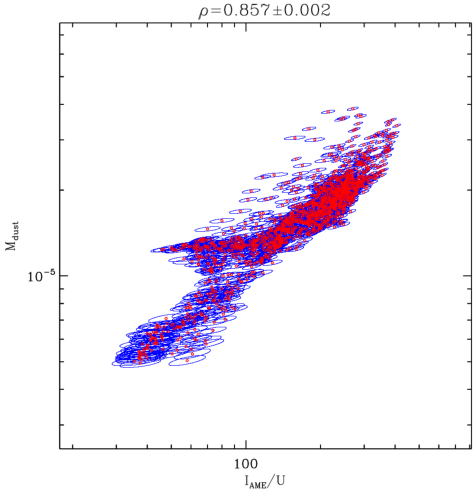
\includegraphics[width=\textwidth]{../Plots/ch_lori/fred_LOri_notes_Oct2017_fig2a.pdf}
                 \centering
                 \caption{Scatter plot with error elipses generated through the Bayesian SED fitting, of total dust mass $M_{dust}$ vs. $I_{AME}$ scaled by $U$.}
                 \label{fig:fred_LOri_notes_Oct2017_fig2a}
               \end{figure}
           AME intensity is scaled by the ISRF intensity $U$. Although spinning dust emission is not predicted to vary directly with $U$, we consider that the ISRF may serve as a diagnostic of environmental conditions in the ISM. In any case, we find that performing such a scaling improves the correlations with dust mass.   Figs.~\ref{fig:fred_LOri_notes_Oct2017_fig2b} and~\ref{fig:fred_LOri_notes_Oct2017_fig2d} describe the variation with $M_{PAH}$ and $M_{PAH+}$.
              \begin{figure}
                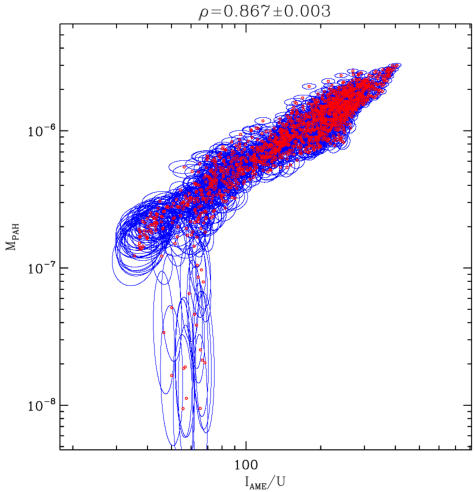
\includegraphics[width=\textwidth]{../Plots/ch_lori/fred_LOri_notes_Oct2017_fig2b.pdf}
                \centering
                \caption{The same comparison is given by~\ref{fig:fred_LOri_notes_Oct2017_fig2a}, but showing total mass of PAHs ($M_{PAH}$) rather than total dust mass on the y-axis. }
                \label{fig:fred_LOri_notes_Oct2017_fig2b}
              \end{figure}
              \begin{figure}
                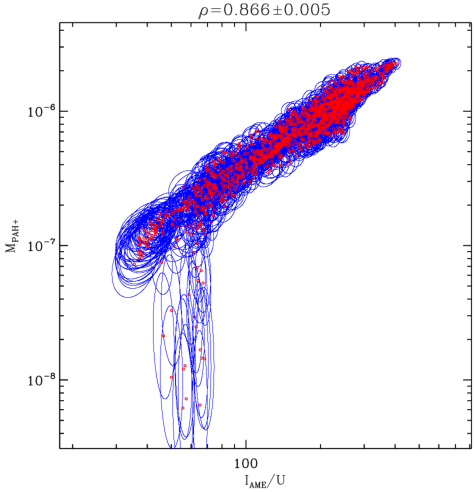
\includegraphics[width=\textwidth]{../Plots/ch_lori/fred_LOri_notes_Oct2017_fig2d.pdf}
                \centering
                \caption{ The same as in Figs.~\ref{fig:fred_LOri_notes_Oct2017_fig2a} and~\ref{fig:fred_LOri_notes_Oct2017_fig2b} , but specifically comparing an estimate of the charged component of PAH mass $M_{PAH+}$. This includes anions and cations, since we cannot distinguish between these two spectroscopically.}
                \label{fig:fred_LOri_notes_Oct2017_fig2d}
              \end{figure}
    Based on the dust properties derived from these SED fits, we investigate whether any fitted parameter shows a preferential relation with the AME. Figs.~\ref{fig:fred_LOri_notes_Oct2017_fig2a}-\ref{fig:fred_LOri_notes_Oct2017_fig2d} reveal a very similar trend between the AME and the parameters $M_{PAH}$, $M_{PAH+}$, and $M_{dust}$. There is a slightly improved correlation between $M_{dust}$ and $M_{PAH}$ (0.857 vs 0.867). This is consistent with the intensity cross correlations in Fig.~\ref{fig:orionis-corr-matrix}. These corrleations are discussed further in Sec.~\ref{sec:lori_discussion} and Fig.~\ref{fig:fred_LOri_notes_Oct2017_fig2c}.

    \subsection{Comparison with unmasked results}
        To assess the effect of applying the mask and background subtraction from Sec.~\ref{sec:dataprocessing}, Figs.~\ref{fig:orionis-img} and \ref{fig:orionis-corr} show a very simplistic version of the image processing. No point-source masking, background adjustment, or missing strip masking are applied. Data are simply smoothed with a 1-degree Gaussian beam, and missing data are interpolated.
          \begin{figure}
            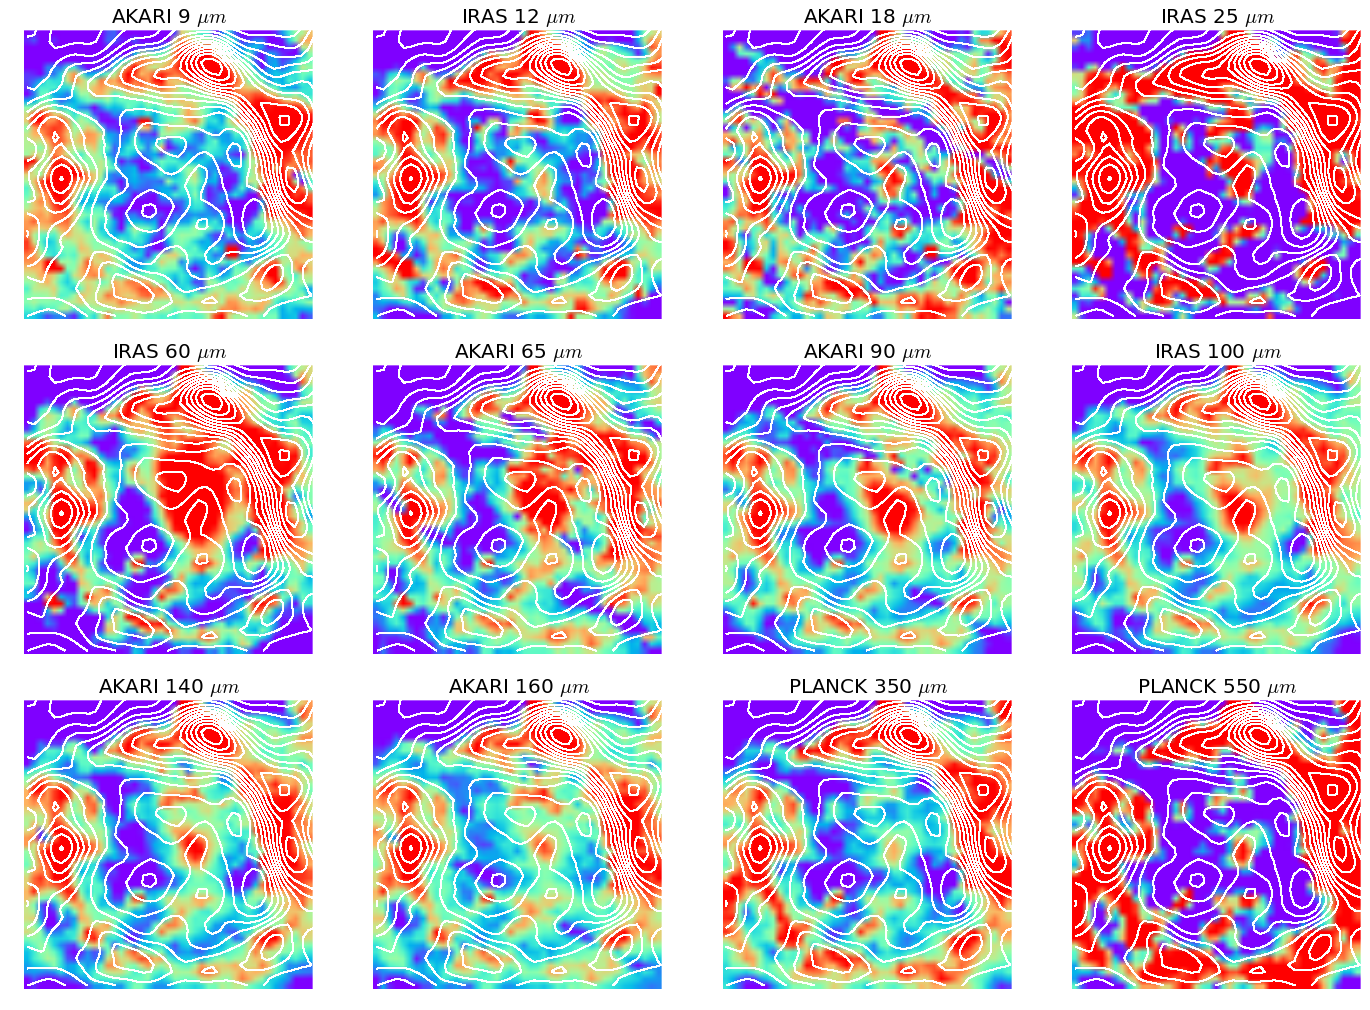
\includegraphics[width=\textwidth]{../Plots/lOrionis_grid_img.png}
            \centering
            \caption{A grid of thumbnails showing the $\lambda$~Orionis region's structure, at 12 wavelengths, along with AME contours (shown in white countours. Spatial correlation seems to be the best at the shortest and longest wavelengths (AKARI/IRC 9~$\mu$m and Planck/HFI 550~$\mu$m). The images are only smoothed and interpolated, for demonstration of the effects without other image processing steps (i.e. background subtraction, point source masking). Figure~\ref{fig:orionis-akari9} demonstrates the actual pixel grid used for the SED fitting and intensity correlation tests.}
            \label{fig:orionis-img}
          \end{figure}
          \begin{figure}
            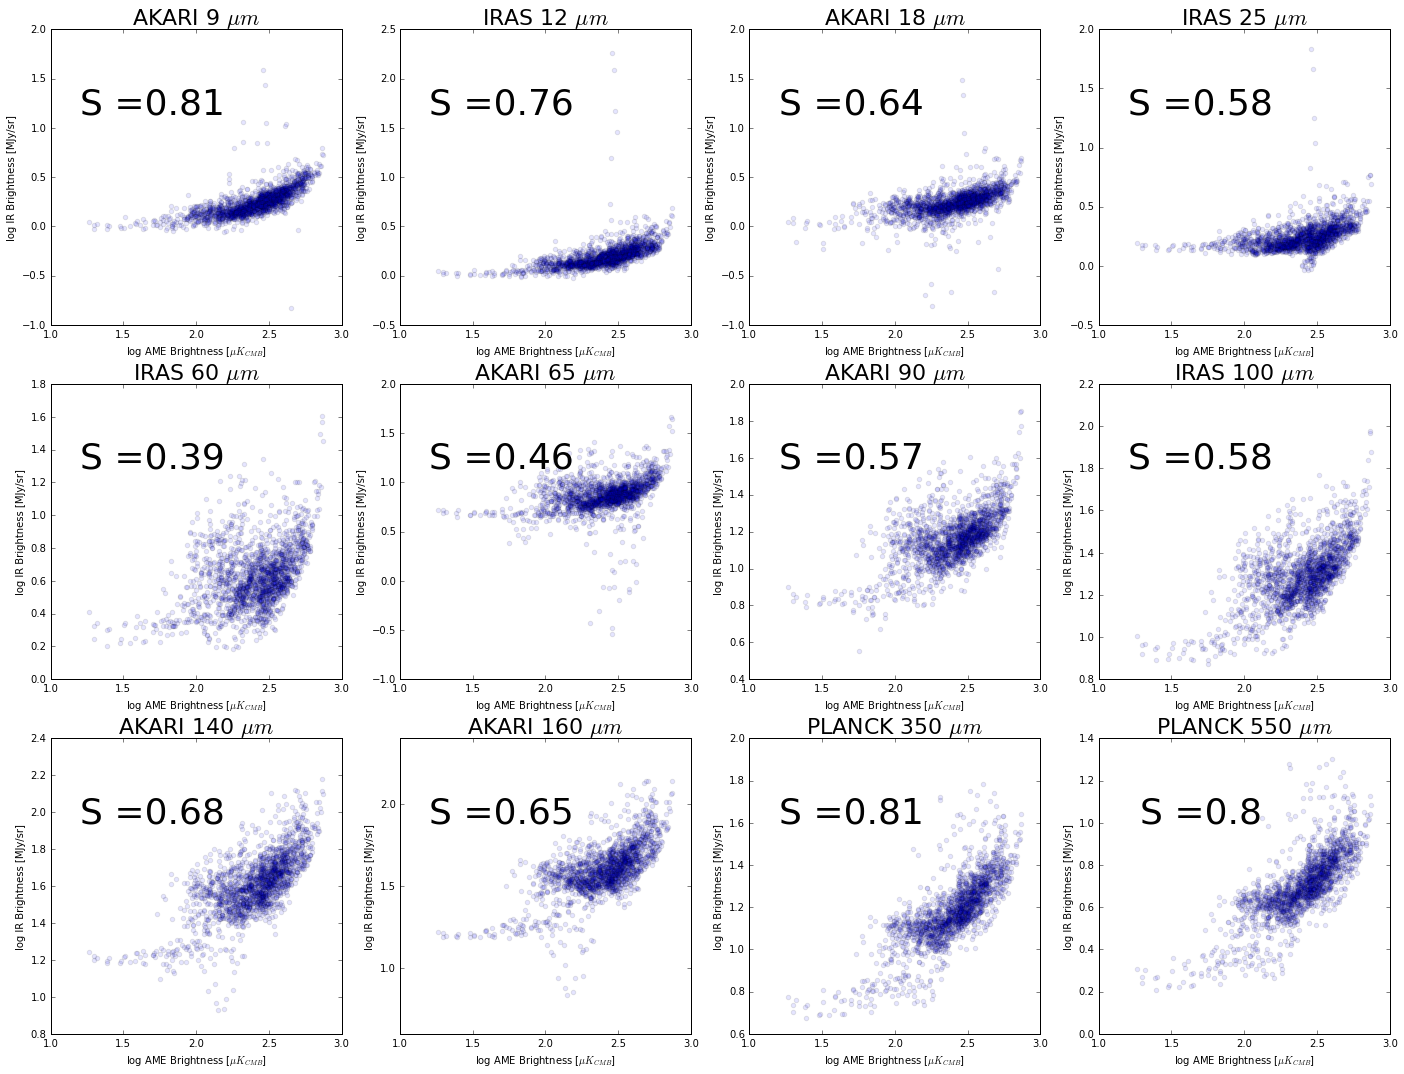
\includegraphics[width=\textwidth]{../Plots/orionis_correlations_AME.png}
            \centering
            \caption{Intensity cross-correlation for all pixels in the $\lambda$~Orionis cut-out region.  $r_{s}$ indicates the Spearman rank correlation coefficient for each plot.}
            \label{fig:orionis-corr}
          \end{figure}
        Contours indicate the region's shape in the PCAME map. Figure~\ref{fig:orionis-corr} shows IR to AME cross correlation plots, for all pixels within the 10$^{\circ}$ by 10$^{\circ}$ $\lambda$~Orionis region. Using this more crude processing, we see in Fig. find the same general pattern--- A9 and P545 show the tightest correlation. Thus the overal result, in terms of a ranking of correlation strengths, does not seem to depend heavily on the image processing steps applied.

  \section{Discussion}
  \label{sec:lori_discussion}
      In  $\lambda$~Orionis we found that accross the whole region, A9 emission and P545 emission were the most strongly correlated with AME. This is apparent both in the photometric band analysis, and in the dust SED fitting.  The fact that the correlation strengths of PAH-tracing mission and sub-mm emission are similar is in-line with what we have seen in \cite{ysard10b} and \cite{hensley16}. In those works, the two relationships (MIR vs. AME and FIR vs. AME) are very close, although these two papers are odds as to which relationship is stronger, and thus in their final interpretation. With the present data and analysis of $\lambda$~Orionis, we fail to rule out PAHs as carriers of the AME. Fig.~\ref{fig:fred_LOri_notes_Oct2017_fig2c} indicates that although total dust mass and PAH mass are both correlated with AME, there is a strong (\textasciitilde{}100\%) probability that PAH mass is the stronger predictor of AME intensity.
          \begin{figure}
            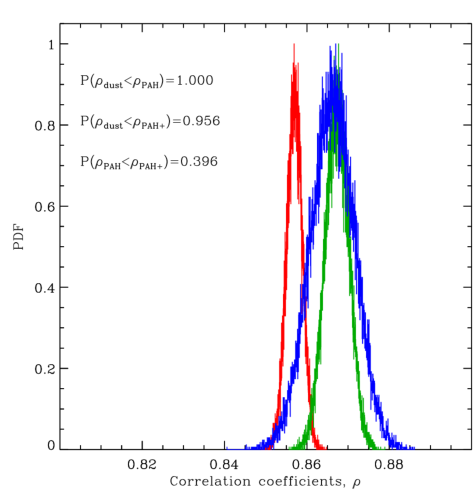
\includegraphics[width=\textwidth]{../Plots/ch_lori/fred_LOri_notes_Oct2017_fig2c.pdf}
            \centering
            \caption{ The Bayesian correlation probablity distributions of Pearson's $\rho{}$) for the three physical parameters vs. the AME intensity: total dust mass, $\rho_{dust}$ (red); total PAH mass $\rho_{PAH}$ (green); and only the ionized PAH mass $\rho_{PAH+}$ (blue). Also given are the probabilities of either PAH component being better correlated with AME than dust mass, as well as the probability that ionized PAH mass correlates better than total PAH.}
            \label{fig:fred_LOri_notes_Oct2017_fig2c}
          \end{figure}
        The results are consistent with a scenario in which PAH mass, cold dust, and the AME are all tightly correlated. A correlation between cold dust and PAHs is observed in extragalactic targets \citep{haas02}, and may be inferred from the correlation between UIR and FIR emission reported in diffuse galactic ISM \citep{onaka96}. In the case that AME emanenates from spinning PAHs, it is not surprising that cold dust would also correlate with the AME. Weaker correlation from 25 to 70~$\mu$m may indicate that AME is weaker in regions of warmer dust and stronger radiation fields. Such an anti-correlation with harsher radiation are consistent with the carriers of AME being destroyed in the central region of $\lambda$~Orionis, thus leading to substantially decreased spinning dust emission.

      \subsection{PAH Ionization fraction}
          As described in Ch.\ref{ch:datasources} it is expected that relative variations between the A9 and I12 intensities could be explained by the fraction of PAHs that are charged, $fPAH+$. Spectroscopically, we cannot distinguish between PAH anions or cations. However if spinning dust emission arises from anions, a better correlation with the mass of charged PAHs $M_{PAH+}$ is expected. However if the PAHs are positively charged, a stronger correlation with $M_{PAH+}$ is not expected. This is due to the rotational excitability of the PAHs: anions are more succeptable to rotational excitation by $H^{+}$ and $C^{+}$ collisions\citep{ali-haimoud10}.

          Examining $\lambda$~Orionis in intensity, we find that the A9 intensity correlates more strongly with AME than I12 or D12. In the $r_{p}$ case, A9 correlates more strongly with AME than any other band. This is consistent with the spinning PAH hypothesis, and taken alone may indicate that the 6.2~$\mu$m feature emission from charged PAHs, may be a better predictor of AME intensity.

          As shown by the dust SED fitting however, the probability distributions (Fig.~\ref{fig:fred_LOri_notes_Oct2017_fig2c}) of $r_{p}(M_{PAH+}:I_{AME})$ do not indicate that ionized PAH mass correlates better with the total PAH mass. Attempts to estimate the $M_{PAH+}$ based on the available data appear to only add noise relative to $r_{p}(M_{PAH}:I_{AME})$. The means of the two distrubtions $r_{p}(M_{PAH+}:I_{AME})$  and $r_{p}(M_{PAH}:I_{AME})$ are similar and $r_{p}(M_{PAH+}:I_{AME})$ shows a wider distribution. Thus the question of whether or not AME comes predominantly from charged PAHs remains open.

          The fact that A9 correlates more strongly than the 12~$\mu$m bands, at least suggests that this topic is worth further investigation. What is clear from the MIR and AME morphology however, is that there is a transition from a relatively PAH depleted, warmer, stronger ISRF in the centerand warm dust in the center to a PAH-supporting region in the ring. Along this transition, there must be a decreasing radiation field with distance from dimnant heating sources, in $\lambda$~Orionis association. \cite{andrews16} predict a transition of PAH species along such a radiation field gradient, from complete PAH destruction in harsh environments, to survival of (sufficiently large) PAH anions near the surface of molecular clouds. Thus if our stronger correlation with A9 indicates charged PAHs, this could be consistent with PAH anions surviving in the portions of $\lambda$~Orionis which are emitting the strongest AME. Future wide-area spectral mapping of the $\lambda$~Orionis region may be able to conclusively test for increased $fPAH+$ in regions with stronger AME. Such studies would eb strongly aided by higher resolution probing of spatial variations the AME spectral profile.

\chapter{All-sky Analysis}
  \label{sec:analysis}
    What we present here is a test of the generalizability of results from Ch.\ref{ch:lori}, which focused on a particular structure on the sky, $\lambda$~Orionis.
    We first would like to note that ``all-sky analysis'' can be a bit misleading. The term tends to lead readers to the idea of a definitive study, answering a particular question for any given position on the sky.  While a truly all-sky analysis would be ideal, signal-to-noise constraints (mainly at high galactic latitudes), as well as confusion along the line of sight (mainly in the galactic plane), make a uniformly powerful study of the whole sky very challenging. Here we will indeed show results for the entire sky as a benchmark analysis, but for the core analysis we must mask certain regions dominated by systematic effects in order minimize biases for particular wavelenghts.

\section{Resolution matching}
    \subsubsection{Smoothing}
        As in Ch.~\ref{ch:lori}, this approach applies to a spatial resolution of approximately \textasciitilde{}$1^{\circ}$. The resolution limimtation is imposed by the PC microwave component maps, which list an `effective resolution' of 60$'$ \citep{planck15X}. Thus we must apply a smoothing to most of our input datasets, which have native resolutions of a much finer scale (see Tab.~\ref{tab:data}), and Fig.~\ref{fig:AME_contours}. The data also come in a wide range of beam shapes with their own degrees of uncertainty, thus we conservatively smooth all of the data in the same way, using a circular Gaussian beam, to have \textasciitilde{}$1^{\circ}$ FWHM resolution. we ar We start with an all-sky AME to IR comparison, looking for global patterns among all pixels.

    \subsubsection{Offset correction}
      The most recent version of the pre-release full-sky IRC data contained an apparent all-sky positive offset of \textasciitilde{}2~MJy/sr for A9 and \textasciitilde{}4~MJy/sr for A18. We assess this offset first by finding the mode of each of the \textasciitilde{}4,700 $3^{\circ}\times3^{\circ}$ tiles of the IRC survey, and then taking the mode of that distribution. We then compare this result with a monopole offset fit to the all-sky HEALPix map of the IRC surveys, built from these tiles. Monopole fitting is handled by the {\tt healpy.fit\_monopole} function. We find the values produced by these two methods to be consistent. We found offsets also in the IRAS, FIS, and HFI bands, thus we apply the same monopole fitting and subtraction to all of the all-sky maps. We do not find the correlation analysis presented in later sections to be sensitive to this offset correction.

  \section{All-sky cross correlations}
        In order to look more closely at how the the AME to IR relationship varies with wavelength, we first do a comparison without applying any pixel mask, as a benchmark. Fig.~\ref{fig:AMEvsDust_allsky_allbands_mpsub_kde_unmasked} shows the pixel-density plots of AME vs. the IR bands' intensities. Darker regions show higher pixel densities, unshaded or more lightly shaded regions show low or zero pixel densities. An intial analysis, considering only the interreations of the PC parameter maps, was presented in Sec.~\ref{sec:PCmaps}, wherein correlations between the major microwave component maps (synchrotron, free-free, AME, and dust emisison) are demonstrated (Fig.~\ref{fig:PCCS_corrmatrix}). This section extends that analysis, considering the full range of IR maps described in Tab.~\ref{tab:data}.

        We see immediately that each band shows evidence of a positive trend with AME intensity. For the MIR bands, at lower IR intensities we see the effects of detector noise become dominant, turning into a more defined positive trend with increasing IR intensity. This effect is less pronounced in the FIR. The trend is similar to that found in Ch.~\ref{ch:lori}, and Fig.~\ref{fig:orionis-corr-matrix}.
          \begin{figure}
            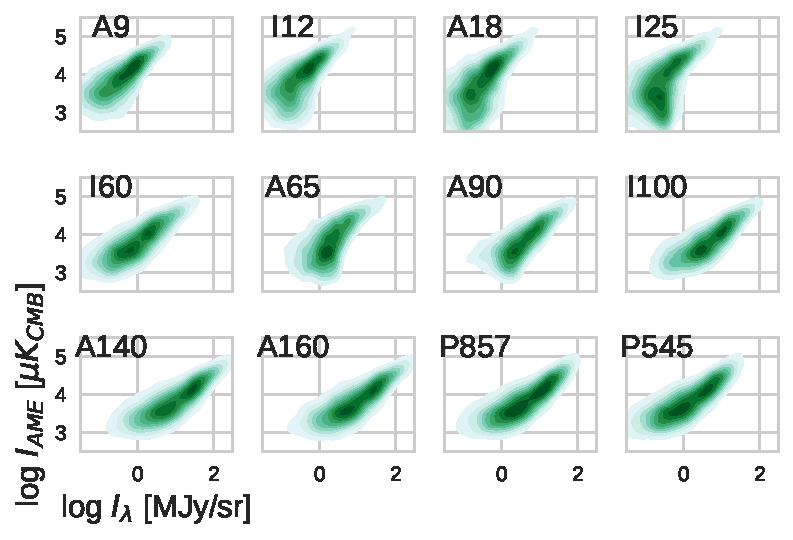
\includegraphics[width=\textwidth]{../Plots/ch_allsky/AMEvsDust_allsky_allbands_mpsub_kde_unmasked.pdf}
            \centering
            \caption{Point-density distributions of the log $AME_{var}$ intensity (Y-axis) vs. log IR bands' intensities. In this case no pixel mask is applied, in order to show overall trend of the full data-set. However a random sampling is used due to computational contraints. The plots show a random set of 20\% of the full-sky data. Darker shaded regions indicate a higher density of pixels.}
            \label{fig:AMEvsDust_allsky_allbands_mpsub_kde_unmasked}
          \end{figure}
        We consider that the IR maps used must not only be compared to the AME, but to each other, to assess multi-wavelength patterns. We also compare the AME and IR maps to ancilliary maps, as decribed in Ch.~\ref{ch:datasources} and Tab.~\ref{tab:ancilliarydata}. Fig.~\ref{fig:all_bands_corr_matrix_wAME_spearman} confirms the weaker trend in the MIR vs. AME, via a cross-correlation matrix, similar to that used in Ch.~\ref{ch:lori} and Fig.~\ref{fig:orionis-corr-matrix}.
          \begin{figure}
            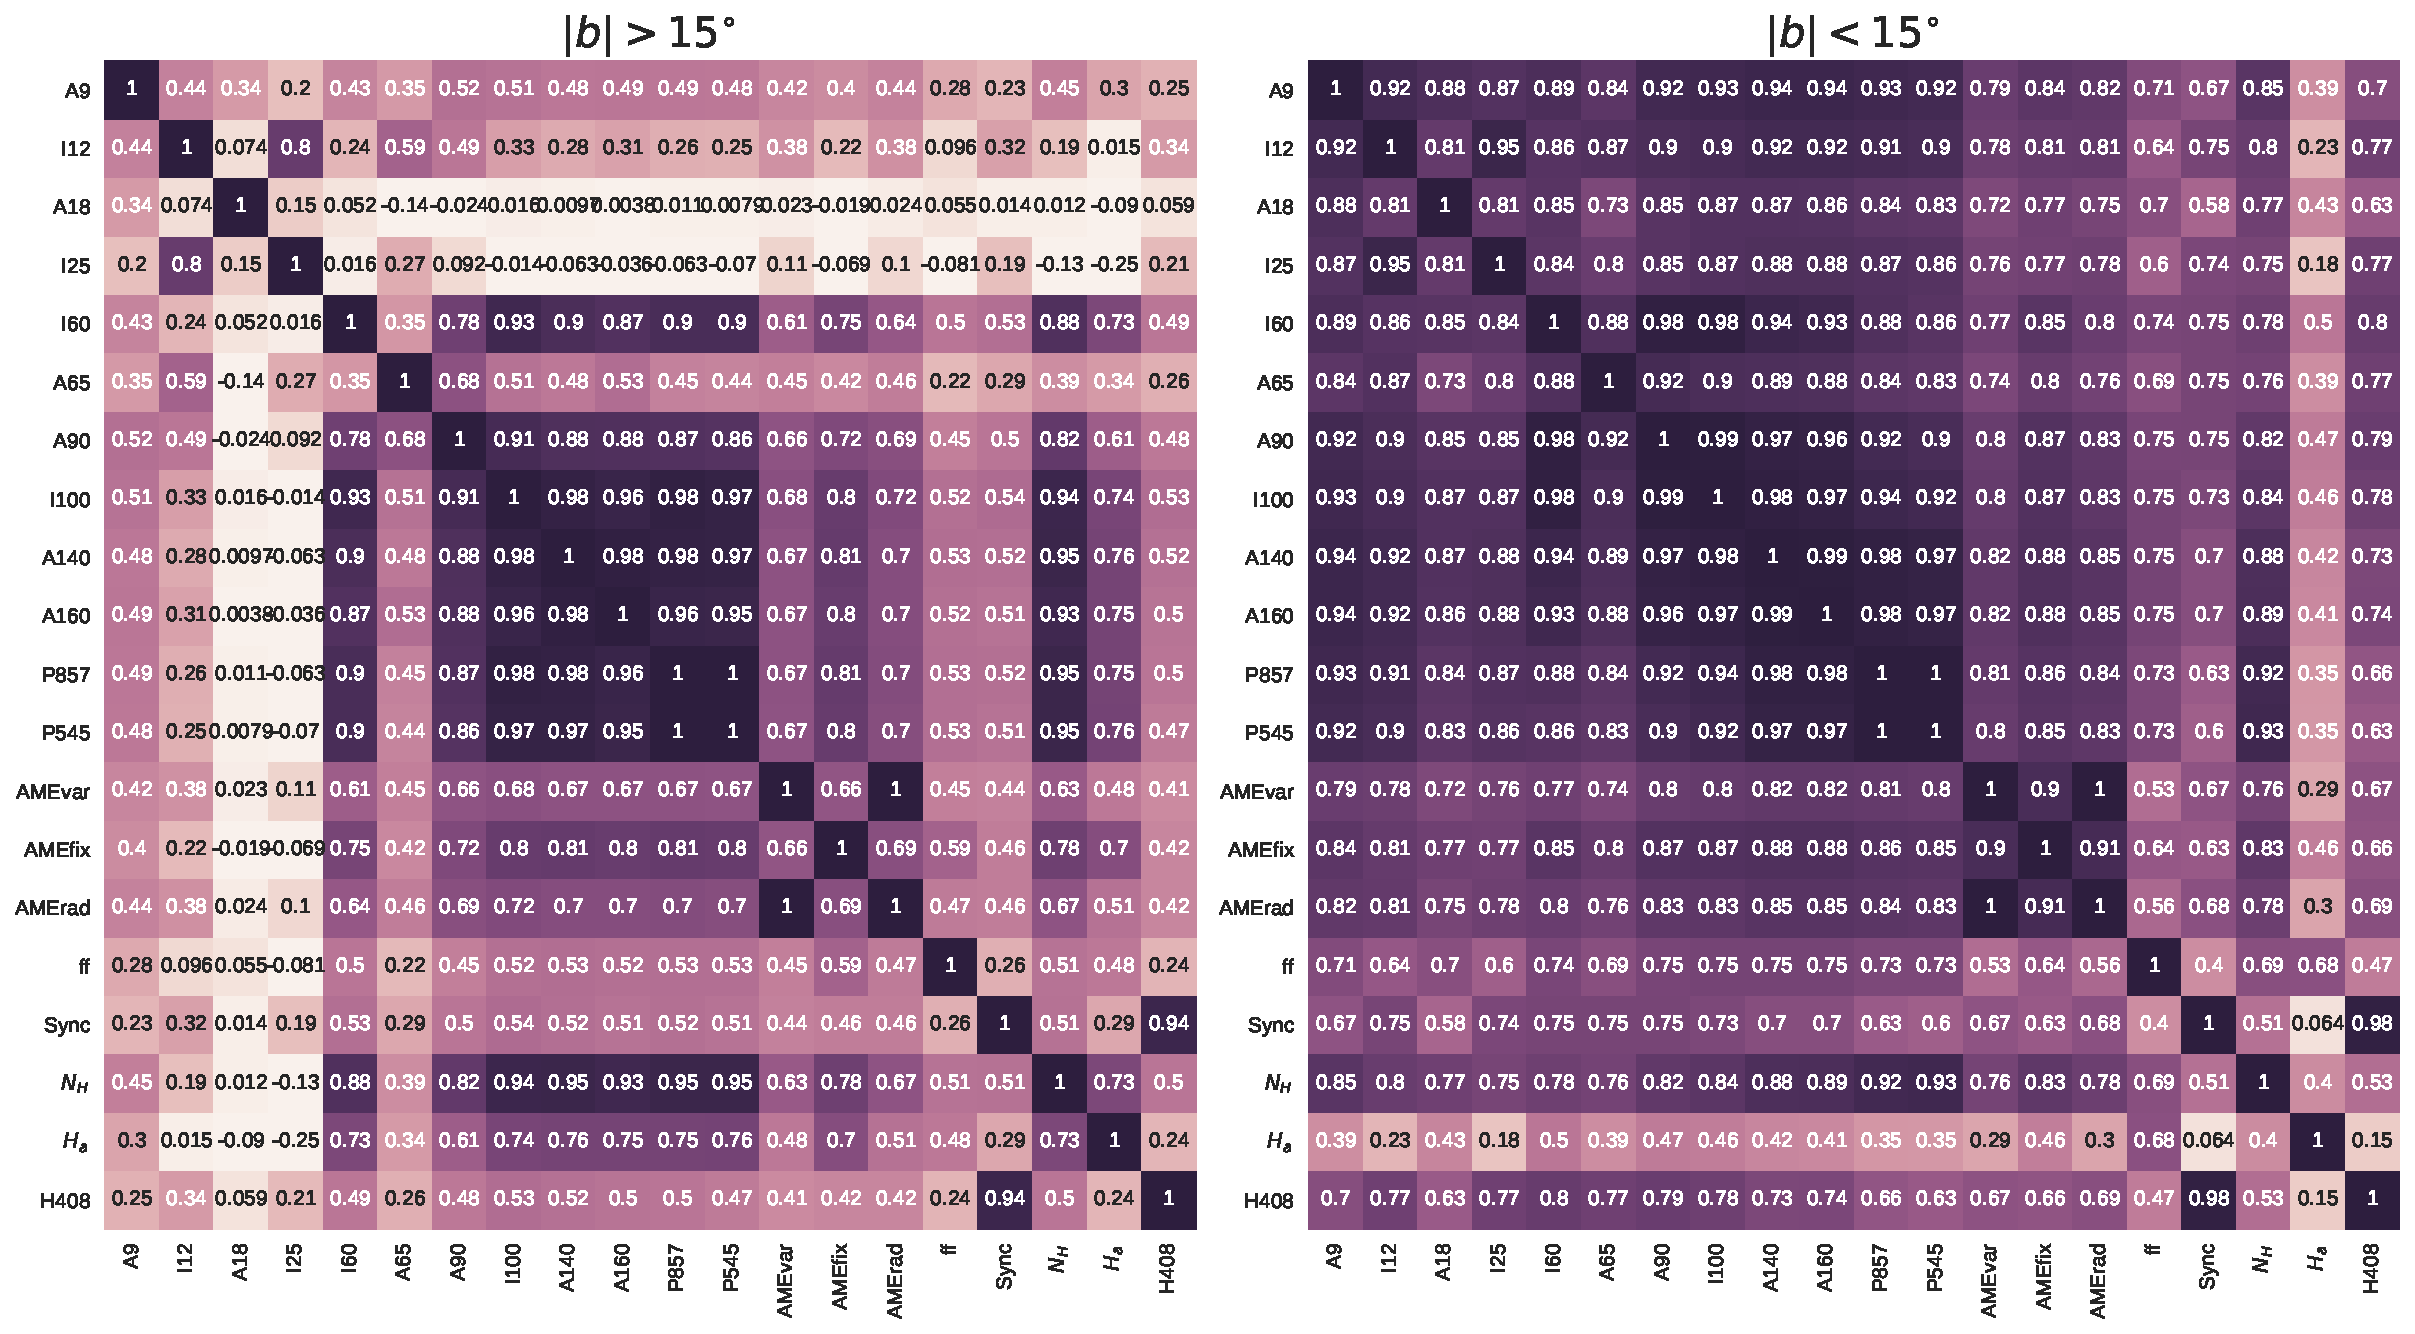
\includegraphics[width=\textwidth]{../Plots/ch_allsky/all_bands_corr_matrix_wAME_spearmanintensity_unmasked.pdf}
            \centering
            \caption{ALL-SKY cross-correlation matrix for the 12 infrared bands sampled, as well as the PC component maps described in Ch.~\ref{ch:datasources}: the two AME components evaluated at their peak frequencies $AME_{var}$, $AME_{fix}$; Syncrotron, and free-free), and ancilliary maps of $N_{H}$, $H{\alpha}$ emission, and 408~MHz emission \cite{haslam82}. The color-scale indicates ($r_{S}$). Results are based on the unmasked sky, but are split by Galaxctic latitude: pixels with $|\beta{}| < 15^{\circ}$ (left) and $|\beta{}| > 15^{\circ}$ (right). The color and annotations indicate $r_{s}$ as in Fig.~\ref{fig:orionis-corr-matrix}. }
            \label{fig:all_bands_corr_matrix_wAME_spearman}
          \end{figure}
       This is reflected in the comparison between high and low latitude plots: for pixels $|\beta| > 15 ^{\circ}$, we see a dramatic effect. In the most extreme case $r_{s}$ of A18 to $AME_{var}$ drops from 0.72 at lower latitudes, to 0.02 at higher latitudes. $r_{s}(A9:AME_{var})$ drops from 0.79 to 0.42. Correlations between the MIR bands and FIR bands also weaken. Only the the interrelations between the FIR bands from I60 to P545 remain essentially latitude independent (with the exception of A65, which has an especially high noise level.)

        In the lower latitudes, with $|\beta| < 15^{\circ}$, bright emission in and around the galactic plane seems to homogenize the bands. We see little change from band to band both in terms of the relationship with AME or with other IR bands. Thus the increase of S/N with decreasing brightness at higher latitudes has a strong effect on such intensity correlation tests. Bands tracing bright thermal dust emission at higher latitudes are more robust against this effect. The only case where the trend is reversed, is with the maps of $N(H)$ and $H{\alpha}$. Both of these maps show higher $r_{s}$ when compared to high latitude FIR emission. The next section descibes a pixel-masking strategy designed to mitigate both $r_{s}$ suppressing effects from band-to-band S/N variations, and $r_{s}$ enhancing effects from confusion near the galactic plane.

      \section{Masked Comparison}
        For the reasons described in the previous section, we consider that an exhaustive comparsion of the AME with IR requires the use of a pixel mask. In this section we describe the various masks applied to the full dataset. We then repeat both the comparisons above (as in  Figs.~\ref{fig:AMEvsDust_allsky_allbands_mpsub_kde_unmasked} and~\ref{fig:all_bands_corr_matrix_wAME_spearman}) for the masked dataset, and present additional analyses. The full mask, superimposed on A9 map, is shown in Fig.~\ref{fig:A9_masked_map}, with the details of the mask layers desribed in the next subsection. The mask most heavily affects high galactic latitudes, and the galactic plane. The same mask is applied to all of the maps.
          \begin{figure}
            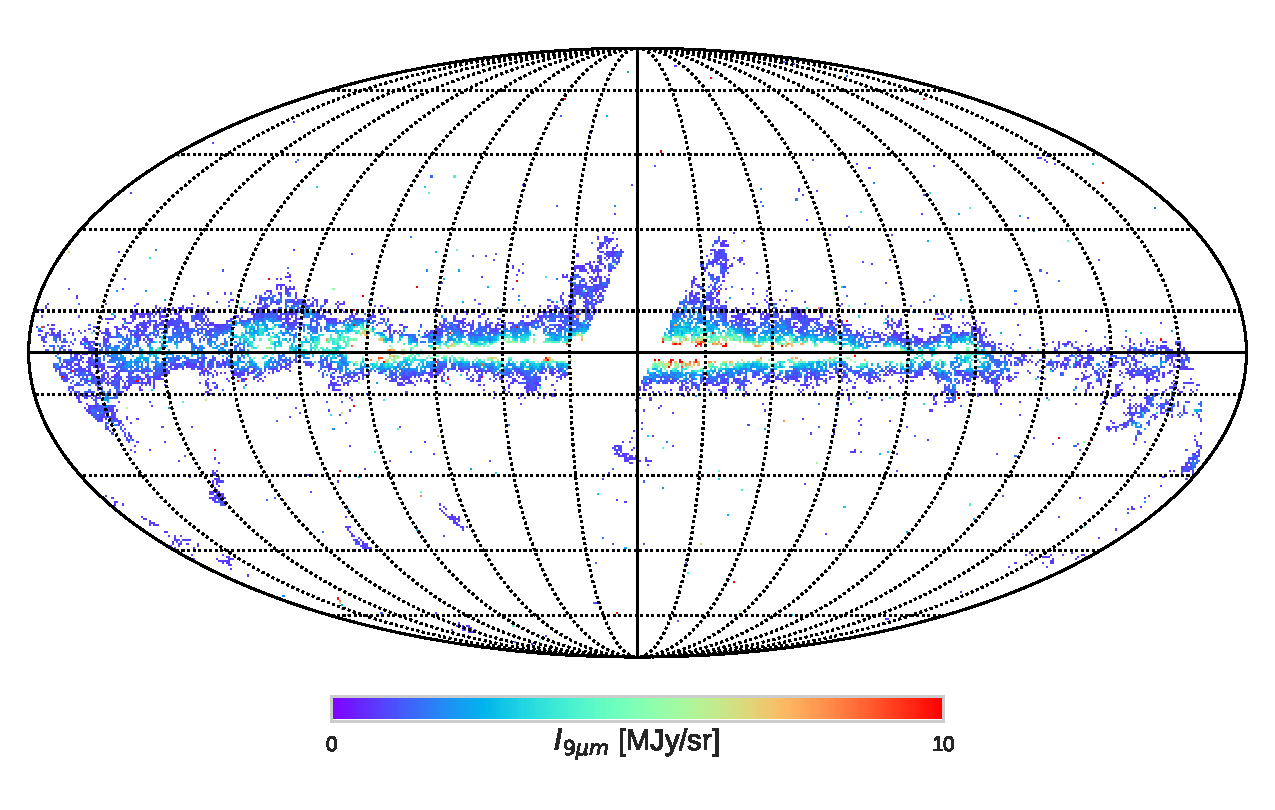
\includegraphics[width=\textwidth]{../Plots/ch_allsky/masked_map_A9.pdf}
            \centering
            \caption{All-sky map in A9 emission after applying the combined masks: ecliptic plane, galactic plane, point sources, and pixels with S/N $<3$. This mask essentially outlines the galaxy, except for the most confused regions. Diffuse galactic emission is essentially removed by the mask due to low S/N in the MIR bands. In the full sky map of \textasciitilde{}700,000 pixels, there are \textasciitilde{}50,000 unmasked pixels remaining.}
            \label{fig:A9_masked_map}
          \end{figure}

      \subsection{Pixel mask}
      \label{sec:pixmask}
        \paragraph{Galactic plane}
          The galactic plane tends to be a challenge in any comparison, but especially with low resolutions studies such as the present work. Complicated structures along the line of sight, smoothed to $1^{\circ}$ resolution, means that emisison within any given pixel is an average of many different environments (evidenced by the homogenizing of the correlations between bands at low latitudes in Fig.~\ref{fig:all_bands_corr_matrix_wAME_spearman}.) Thus we exclude the brightest emission of the galactic plane, according to the mask prepared by the Planck Collaboration.

        \paragraph{Zodical light}
          To minimize the effects of residual zodiacal light, we exclude pixels within $10^{\circ}$ of the ecliptic plane.  Even though we use the Zodi-subtracted maps \citep{kelsall98, kondo16, ootsubo16}, the Zodi residuals are still problematic (especially in the MIR.) This corresponds to regions with the heaviest contamination from Zodiacal light, where Zodi residuals are apparent even with visual inspection for all of the MIR bands used in this study. In Ch.~\ref{ch:datasources}, Figs. \ref{fig:ratioMap_A9I12}, and \ref{fig:ratioMap_A9I12} clearly display these residual patterns.

        \paragraph{Signal to noise}
          Some of the bands used lack sufficient sensitivity to trace fainter emisison, especially at higher galactic latitudes. This is mainly an issue for the mid-infrared bands. As such, we enforce a 3$\sigma$ threshold for all of the maps--- adding to the mask any pixel that has lower than 3$\sigma$ detection in any of the maps. This removes nearly all pixels beyond approx. $15^{\circ}$ from the galactic plane, with the pronounced exception of regions affected by stray moonlight. The extent of this particular mask is primarily defined by the IRC A9 and A18 maps, which have the highest noise levels.

       \paragraph{Point Sources}
         The Planck Collaboration provides masks of the pixels they find to include point sources. We mask pixels which are flagged as being point-source contaminated, in the most heavily affected maps: Planck/HFI~857 GHz and Planck/LFI~30 GHz.

      \paragraph{PC Component Separation Errors}
        As noted in \cite{planck15X, hensley16}, there are fluctuations in the PC maps wherein AME emission appears to correspond to fluctuations in the synchrotron map. While a mask of all but the most reliably component separated pixels would be ideal, the construction of such a mask with the current data would require us to use a rather artificial threshold. While PC does provide error maps for each of the components, these are not necessarily an indication of how confident the component separation process itself is at a given pixel. We prefer not to apply any additional masks tailored to the PC maps, and instead present and discuss the results with the possibility of component separation artifacts in mind. However we do note that applying the LFI point source mask and galactic plane masks serves also to mask most pixels with AME peak frequency outliers.

        \subsection{Effect of mask application}
            Fig.~\ref{fig:AMEvsDust_allsky_allbands_mpsub_kde_masked} shows point-density plots for $AME_{var}$ vs. each of the IR bands, after applying the mask described above.
               \begin{figure}
                 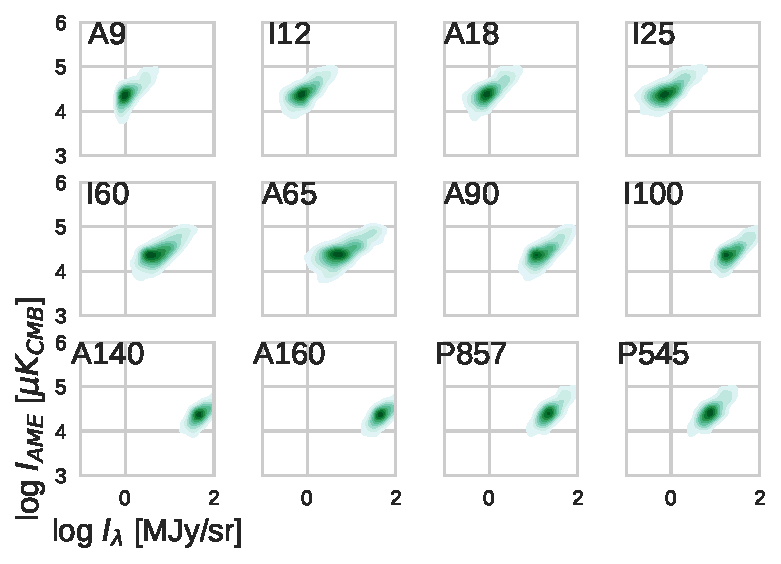
\includegraphics[width=\textwidth]{../Plots/ch_allsky/AMEvsDust_allsky_allbands_mpsub_kde_masked.pdf}
                 \centering
                 \caption{The same comparison as shown for Fig.~\ref{fig:AMEvsDust_allsky_allbands_mpsub_kde_unmasked}, but with the mask applied as in Fig.~\ref{fig:A9_masked_map}.}
                 \label{fig:AMEvsDust_allsky_allbands_mpsub_kde_masked}
               \end{figure}
            As expected with such a drastic reduction of the number of noise-dominated points, the scatter, especially for the MIR bands, is reduced. This can be seen by comparing the Fig.~\ref{fig:AMEvsDust_allsky_allbands_mpsub_kde_masked} to the unmasked distributions vs. AME in Fig.~\ref{fig:AMEvsDust_allsky_allbands_mpsub_kde_unmasked} Otherwise the applicaiton of the mask does not bring about any special distinction among the bands when compared to the AME. What is notable however is that the persistent weakening of trend of I25 vs. AME, relative to A9 and the FIR bands. This is seen also when looking at the full set of interrelations via the cross-correlation matrix in Fig.~\ref{fig:all_bands_corr_matrix_wAME_spearmanintensity_maskall}.
              \begin{figure}
                 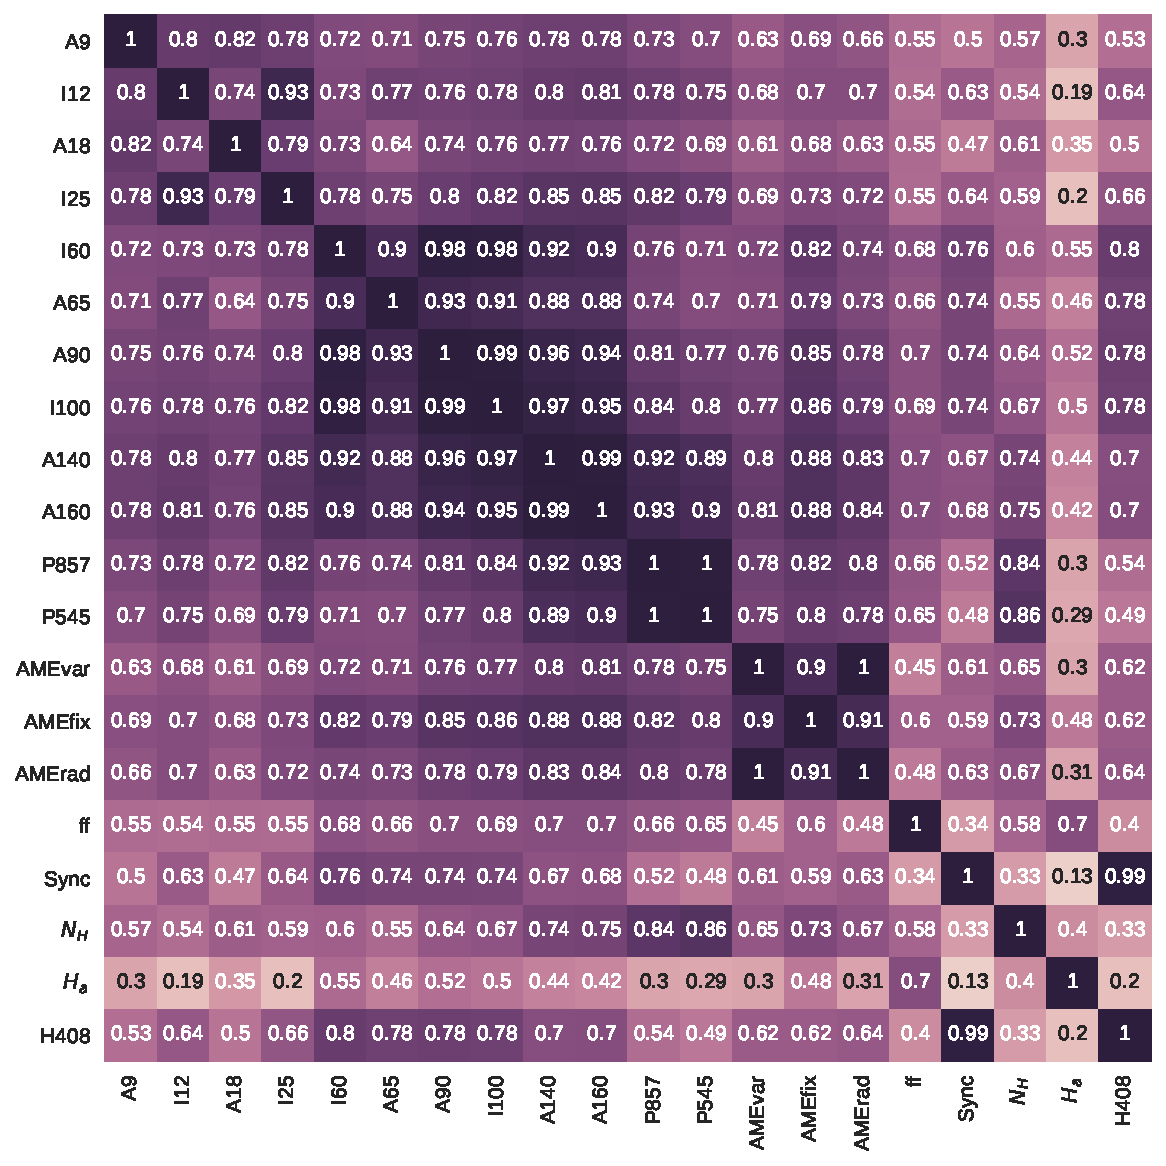
\includegraphics[width=\textwidth]{../Plots/ch_allsky/all_bands_corr_matrix_wAME_spearmanintensity_maskall.pdf}
                 \centering
                 \caption{Cross-correlation ($r_{s}$ matrix for the IR intensities (unscaled) vs. each other, esssentially the same comparison as in Fig.~\ref{fig:all_bands_corr_matrix_wAME_spearman}, except that the pixel mask is applied, and we do not perform a split by Galactic latitude--- after the mask is applied, over 90\% of pixels are within $10^{\circ}$ of the galactic plane.}
                 \label{fig:all_bands_corr_matrix_wAME_spearmanintensity_maskall}
              \end{figure}

        \paragraph{Normalizing by radiation field $U$}
          Following the logic that the PAH-tracing bands intensity is essentially a product $U$ and the column density of PAHs $\sigma_{PAH}$ (as explained in Ch.~\ref{ch:datasources}), we redraw the comparison after scaling the MIR bands by $U$. We determine $U$ by taking the $1^{\circ}$-smoothed, degraded PR1 dust radiance map (also used in \citep{hensley16}), and its corresponding $\tau_{353}$ map. We approximate $U \propto R/\tau_{353}$. In the case of $U$-normalized intensities correlation plots, we only include the MIR bands. While $I_{MIR}/U$ is thought to trace column density of the band carriers (PAHs, or VSGs), there is a less definite interpretation of $I_{FIR}/U$ (since the profile of FIR dust emission depends on the dust temperature.) Thus for this particular comparison, we represent the FIR with $\tau_{353}$. The $U$-normalized correlation matrix is given by Fig~\ref{fig:all_bands_corr_matrix_wAME_spearmanU_norm_masked}.
                \begin{figure}
                    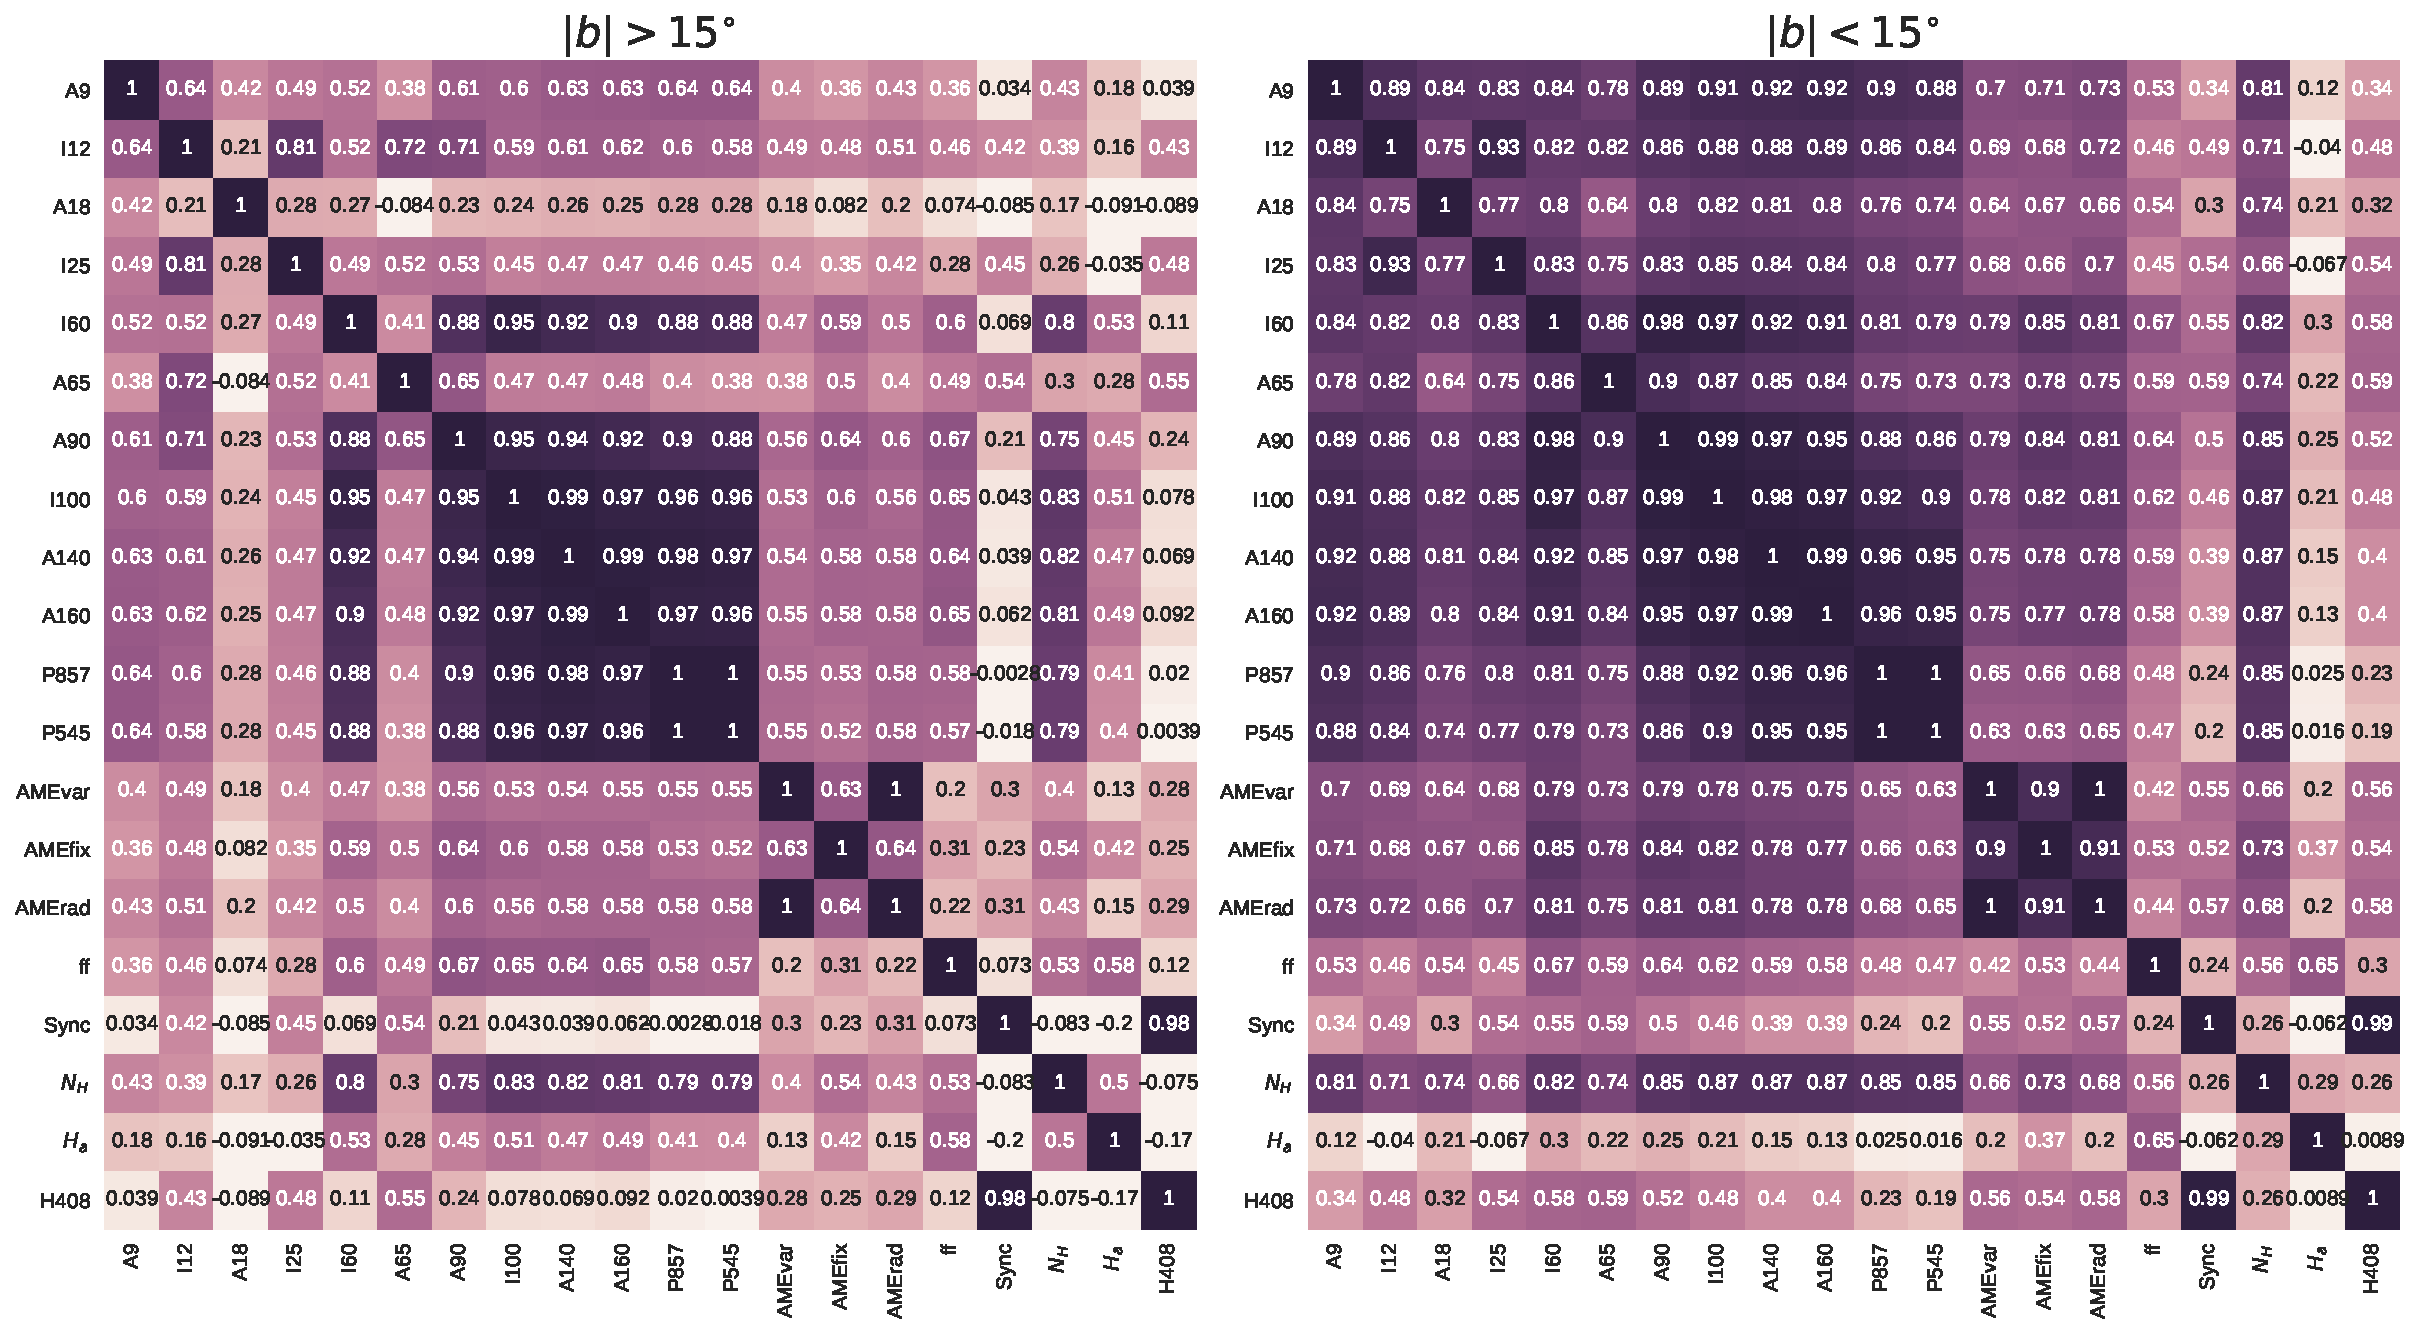
\includegraphics[width=\textwidth/2]{../Plots/ch_allsky/all_bands_corr_matrix_wAME_spearmanU_norm_masked.pdf}
                    \centering
                    \caption{Cross-correlation ($r_{s}$ matrix for the $U$-normalized IR intensities vs. each other, and also against the AME components, other PC products, and ancilliary data. Only the IR maps are divided by $U$- other data is unchanged from Fig.~\ref{fig:all_bands_corr_matrix_wAME_spearmanintensity_maskall})}
                    \label{fig:all_bands_corr_matrix_wAME_spearmanU_norm_masked}
                \end{figure}
            In this comparison, we see that all of the correlations of the MIR bands vs. AME weaken slightly when we scale the MIR bands by $U$. However if we consider that $U$ may also affect the AME intensity, it may make sense to show a comparison where the MIR bands and AME intensities are all scaled by $U$. Fig.~\ref{fig:all_bands_corr_matrix_wAME_spearmanU_norm_AMEnorm_masked} shows such a comparison, and indeed the correlations improve slightly.
                \begin{figure}
                    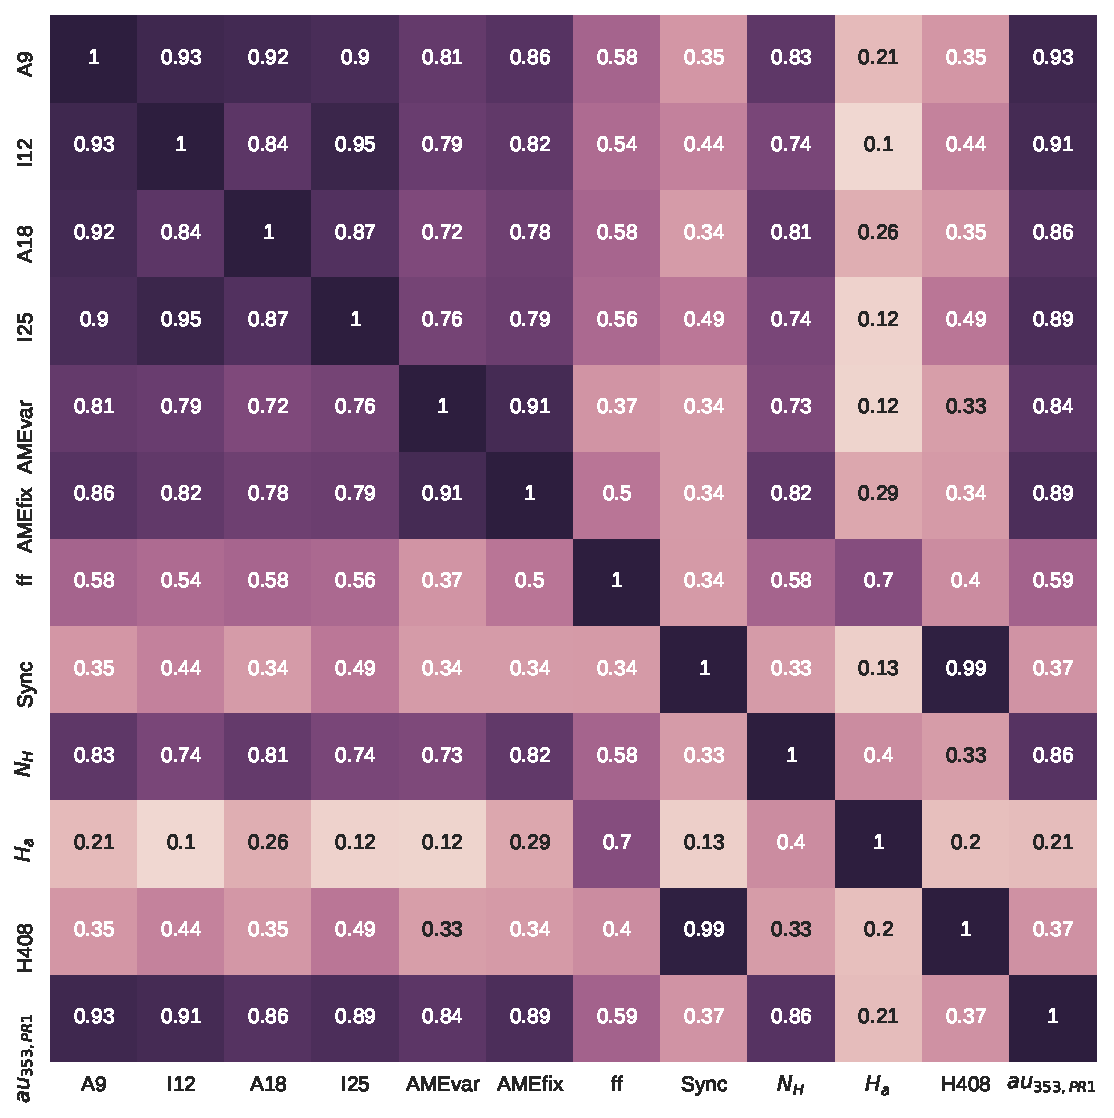
\includegraphics[width=\textwidth/2]{../Plots/ch_allsky/all_bands_corr_matrix_wAME_spearmanU_norm_AMEnorm_masked.pdf}
                    \centering
                    \caption{Cross-correlation ($r_{s}$ matrix for the $U$-normalized IR intensities vs. each other, and also against the AME components, other PC products, and ancilliary data. Only the IR maps are divided by $U$- other data is unchanged from Fig.~\ref{fig:all_bands_corr_matrix_wAME_spearmanintensity_maskall})}
                    \label{fig:all_bands_corr_matrix_wAME_spearmanU_norm_AMEnorm_masked}
                \end{figure}
            In fact, scaling both the MIR and AME intesities by $U$ gives a stronger correlation than even the unscaled case shown in Fig.~\ref{fig:all_bands_corr_matrix_wAME_spearmanintensity_maskall}.


        \paragraph{R-normalized comparison}
            For completeness we perform a comparison similar to that provided in \cite{hensley16}, wherein they compared the ratio $I_AME/R$ to the fraction of dust in PAHs, $fPAH$. In our analysis, the ratios of $A9/R$ and $I12/R$, considering that A9 and I12 are dominated by PAH emission, would be comparable to the \cite{hensley16} parameter of $fPAH$.
                \begin{figure}
                    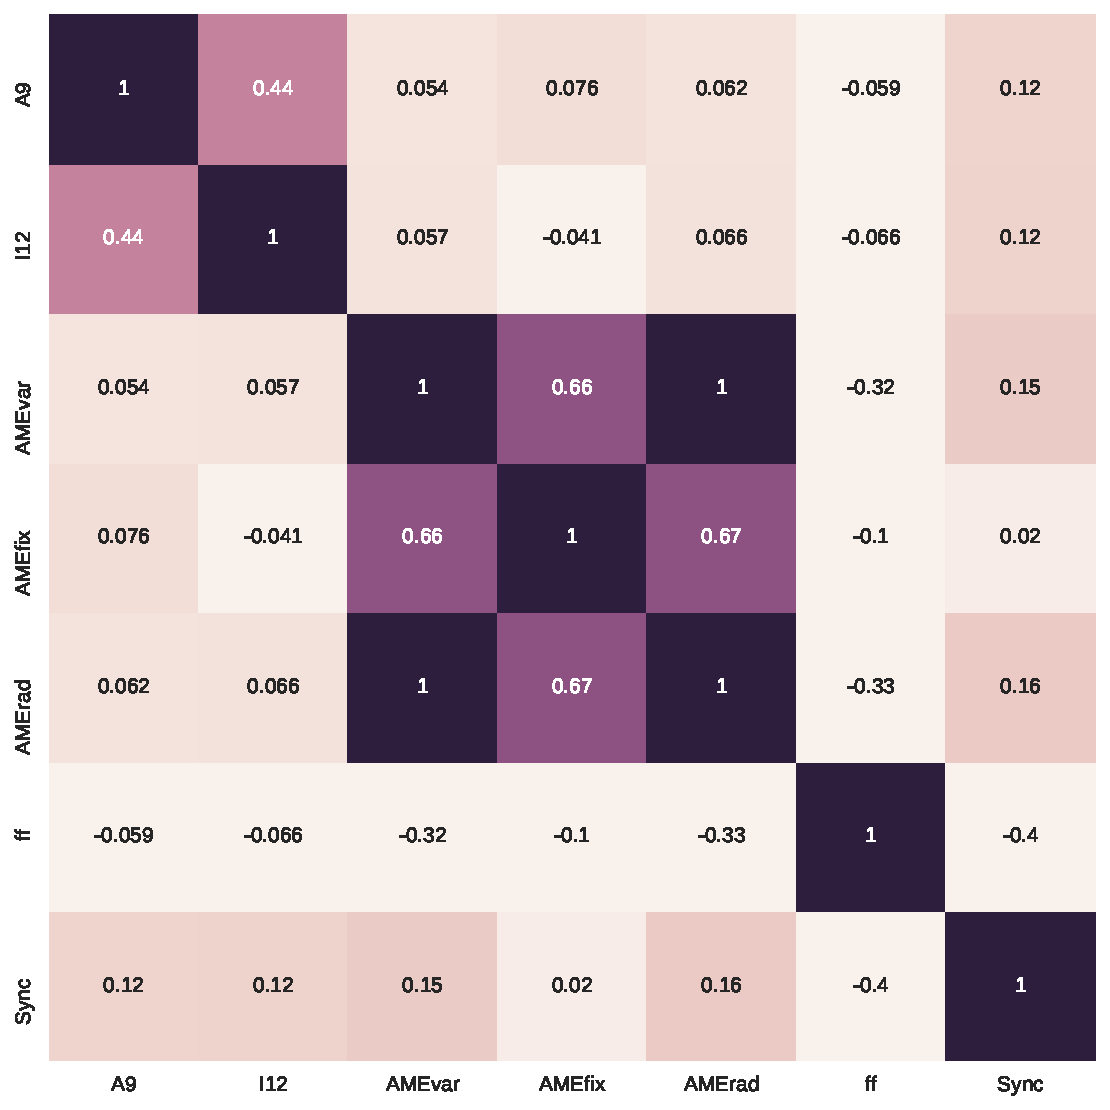
\includegraphics[width=\textwidth/2]{../Plots/ch_allsky/all_bands_corr_matrix_wAME_spearmanR_norm_masked_hens.pdf}
                    \centering
                    \caption{Cross-correlation ($r_{s}$ matrix for the $R$-normalized IR intensities vs. each other. )}
                    \label{fig:all_bands_corr_matrix_wAME_spearmanR_norm_masked_hens}
                \end{figure}
            As with the result in \cite{hensley16}, these data do not reveal any correlation between PAH fraction and $I_{AME}/R$, or with any of the MIR/R ratios and $I_{AME}/R$. Interestingly, there is evidence of a marginal positive trend with synchrotron, and a negative trend with free-free emission.

          \paragraph{Bootstrap test}
              In addition, for the masked comparison, we carry out a boostrap analysis, using the same method explained in Ch.~\ref{ch:lori}. The Spearman rank correlation coefficents $r_{S}$ of all of the bands, in intensity, vs. the $AME{var}$ component are shown. This is done only for the masked case, due to the computational challeneges presented by a well-sampled bootstrap of all \textasciitilde{}780,000 pixels in the full sky. Because the mask applied here leaves us with approximately 1/7 of the sky, a bootstrap with $N_{iterations} > N_{pix}$ becomes tractable. We show the comparison only for the $AME_{var}$ component also due to computational constraints. The $r_{s}$ distributions for each IR band vs. AME are shown in Fig.~\ref{fig:bootstrap_vs_AME_allsky_masked}.
                \begin{figure}
                     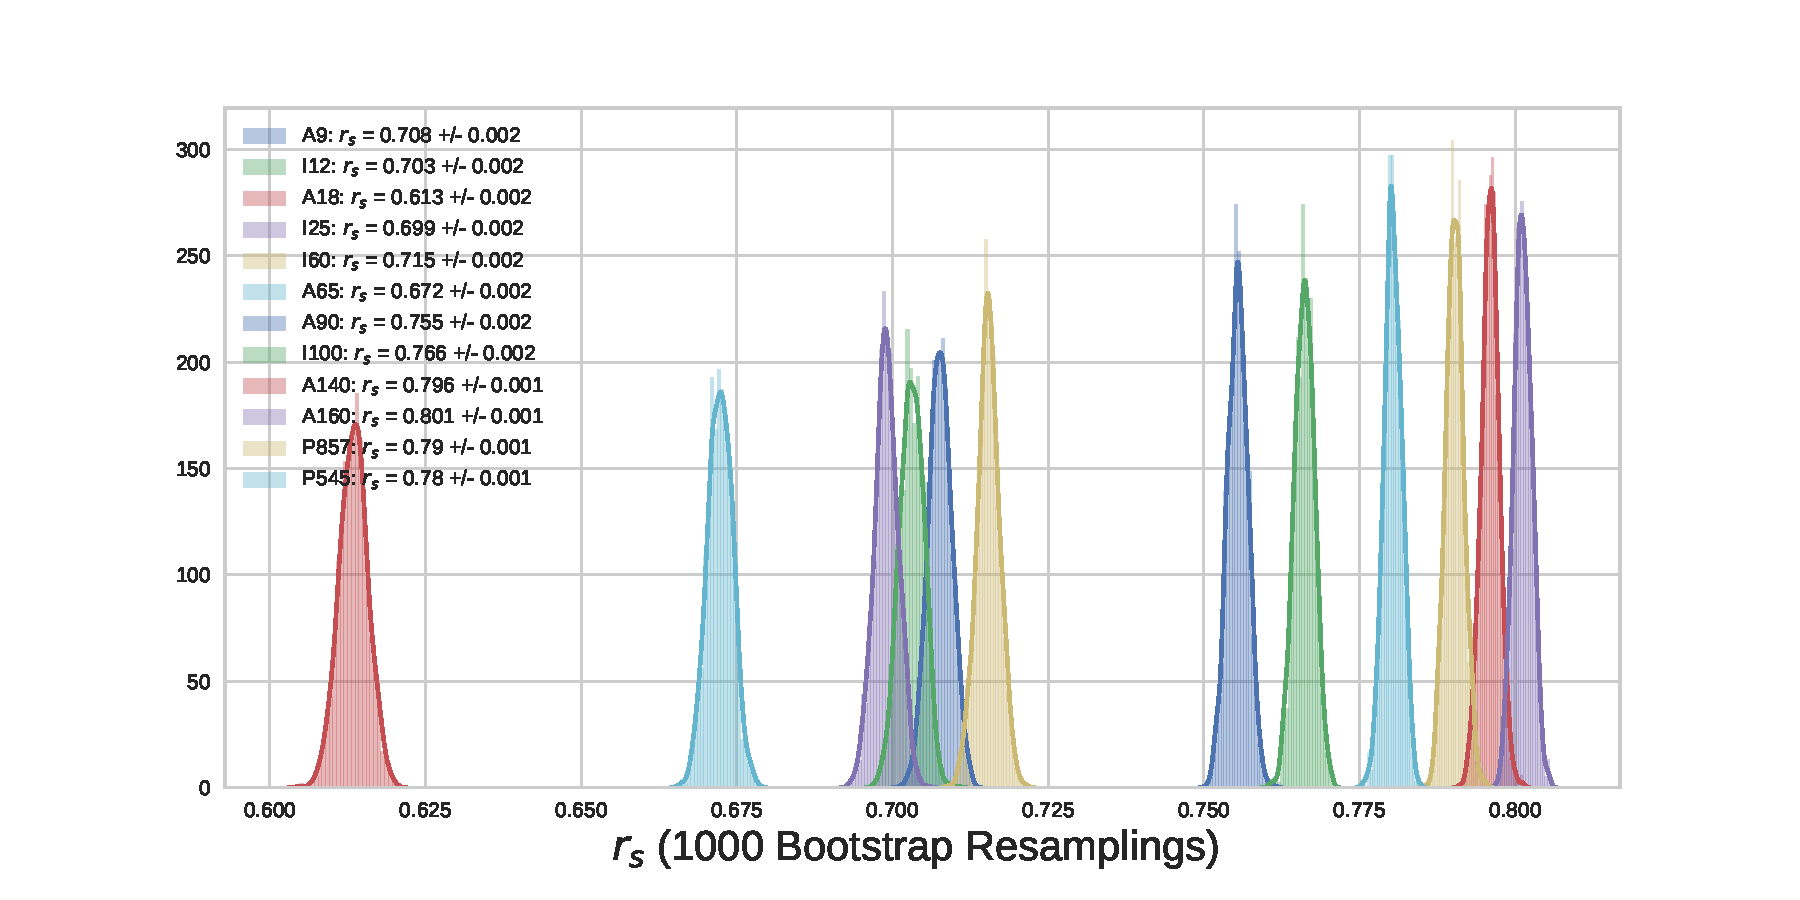
\includegraphics[width=\textwidth,trim={3cm 0.25cm 2.5cm 1cm},clip]{../Plots/ch_allsky/bootstrap_vs_AME_spearman_maskall_i1000.pdf}
                     \centering
                     \caption{Re-sampled (Bootstrap) correlation tests for IR emission vs. AME, performed on the masked all-sky maps. Each band's $r_{s}$ distribution is shown in a different color. The width of the distribution indicates the error for the given data in the correlation coefficient. The mean and standard deviation of the scores are given in the legend of each plot. The plot ranges only show positive values, since no negative scores were produced. }
                     \label{fig:bootstrap_vs_AME_allsky_masked}
                \end{figure}
            The calculations are performed in the same way as with Fig.~\ref{fig:bootstrap_vs_AME} for $\lambda$~Orionis. Consistent with the other correlation analyses already shown in this chapter, there is a stronger correlation in the FIR, espeically A160. Considering the MIR range, and as with $\lambda$~Orionis, A9 emission correlates better than I12. The worst correlation is seen with the A18 and I25 bands.
\section{Spatial variation of correlations}
    To understand how these trends may vary across the sky, independent from the choice of pixel masl, we produce an all-sky maps of $r_{s}$ for AME vs. IR emission. From the NSIDE~256 input maps of AME and 4 IR wavelength maps, we produce NSIDE~8 maps of $r_{s}$. These maps are shown in Figs.~\ref{fig:Spearman_Map_nside8_AMEvartoIR_A9}-\ref{fig:Spearman_Map_nside8_AMEvartoIR_A140}
      \begin{figure}
        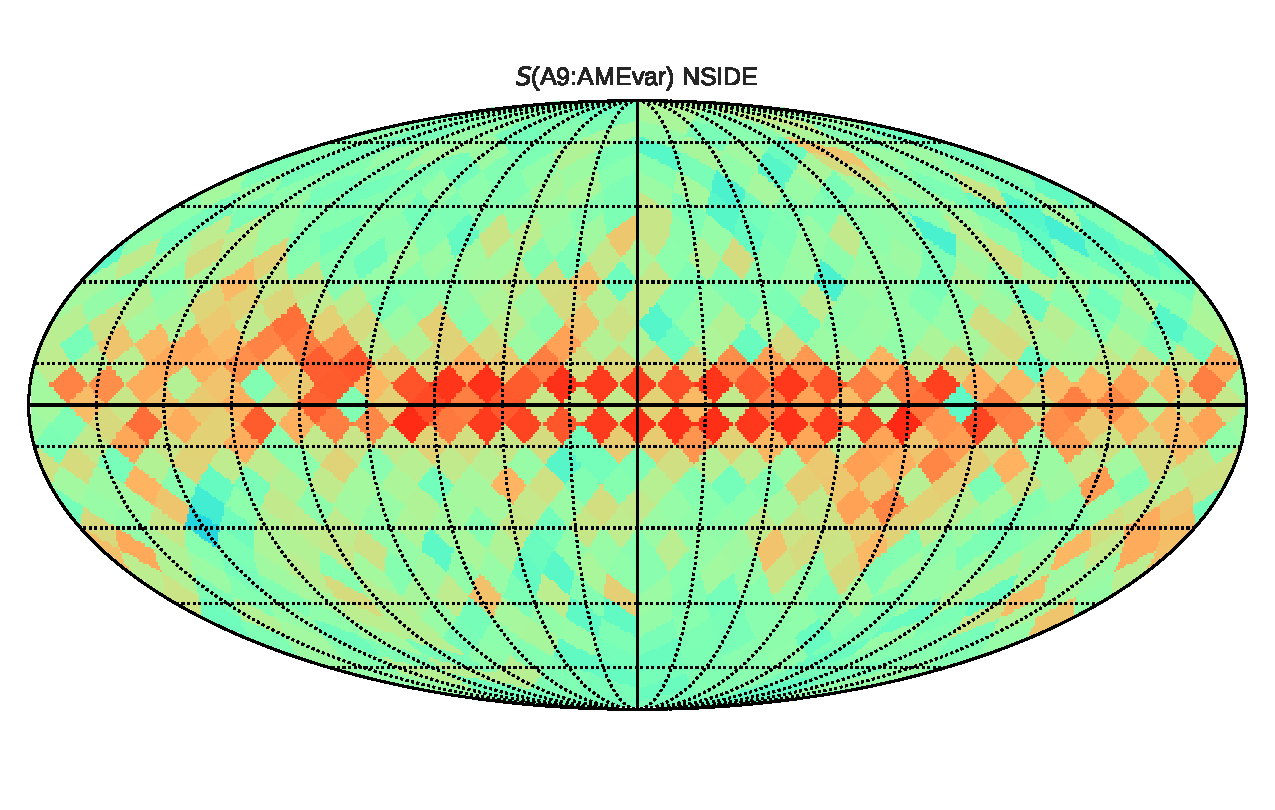
\includegraphics[width=\textwidth/2]{../Plots/Allsky_Corr/Spearman_Map_nside8_A9toAMEvar.pdf}
        \centering
        \caption{Spatial map of $r_{s}$ between the AME and IR intensity for A9. $r_{s}$ is calculated for all NSIDE~256 pixels within each NSIDE~8 pixel-sized bin. The correlation score is calculated with the unmasked maps. The colorbar indicates $r_{s}$, ranging from -1 (negative monotonic relationship) to +1 (positive monotonic relationship).}
        \label{fig:Spearman_Map_nside8_AMEvartoIR_A9}
      \end{figure}
      \begin{figure}
        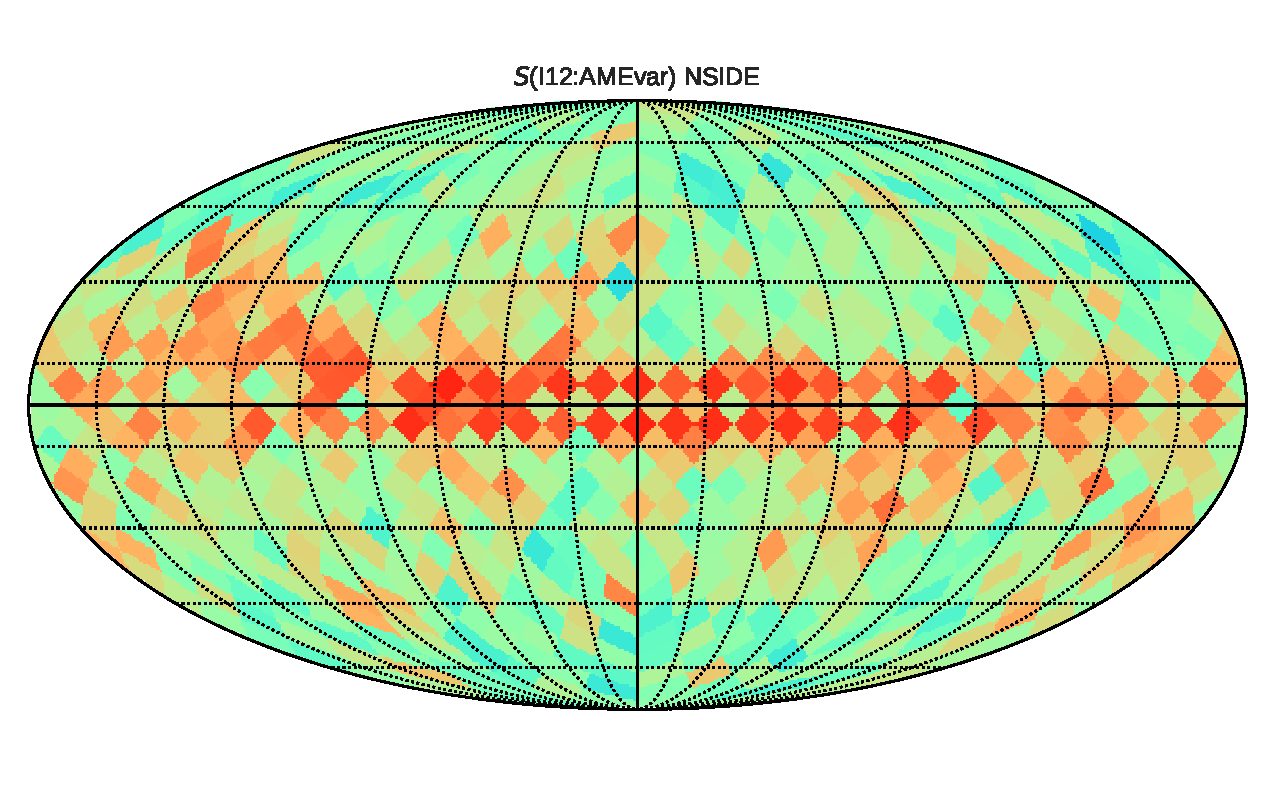
\includegraphics[width=\textwidth/2]{../Plots/Allsky_Corr/Spearman_Map_nside8_I12toAMEvar.pdf}
        \centering
        \caption{Spatial map of $r_{s}$ between the AME and IR intensity for I12, calculated as in Fig.~\ref{fig:Spearman_Map_nside8_AMEvartoIR_A9}.}
        \label{fig:Spearman_Map_nside8_AMEvartoIR_I12}
      \end{figure}
      \begin{figure}
        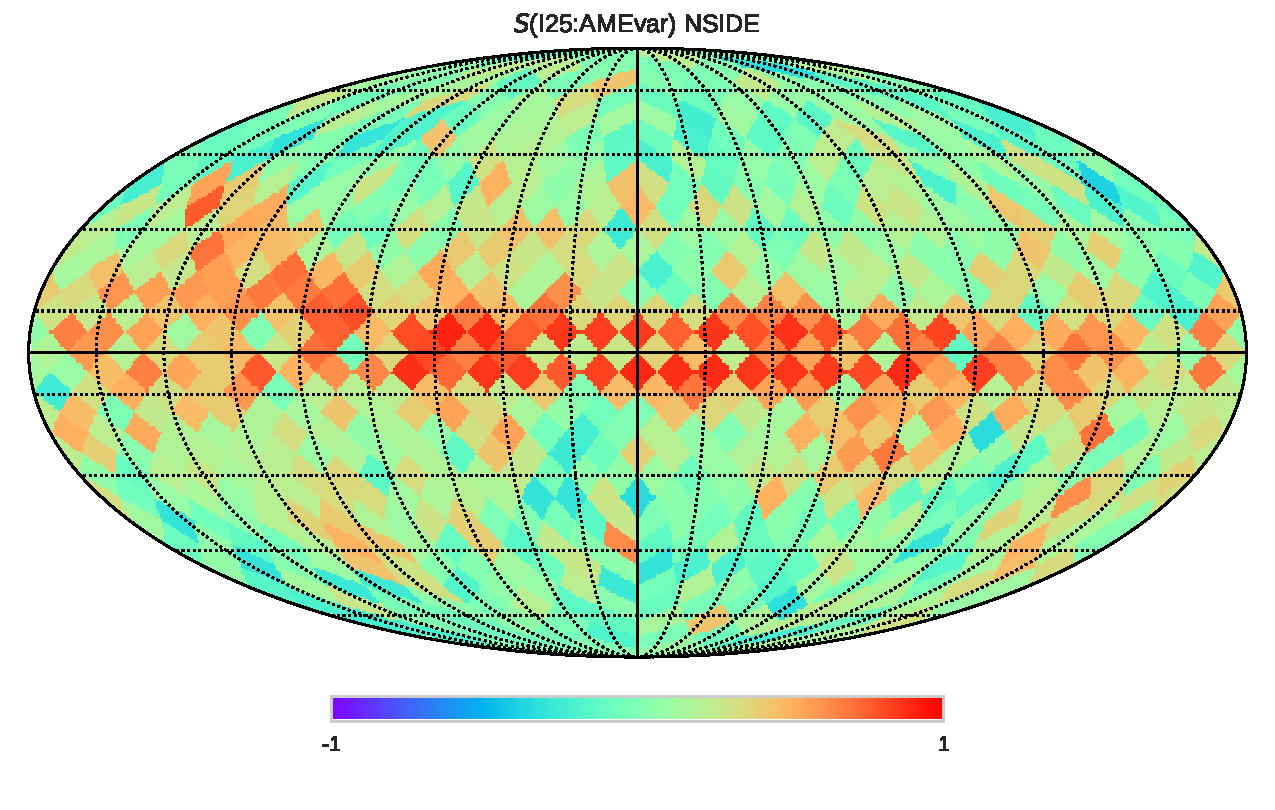
\includegraphics[width=\textwidth/2]{../Plots/Allsky_Corr/Spearman_Map_nside8_I25toAMEvar.pdf}
        \centering
        \caption{Spatial map of $r_{s}$ between the AME and IR intensity for I25, calculated as in Fig.~\ref{fig:Spearman_Map_nside8_AMEvartoIR_A9}.}
        \label{fig:Spearman_Map_nside8_AMEvartoIR_I25}
      \end{figure}
      \begin{figure}
        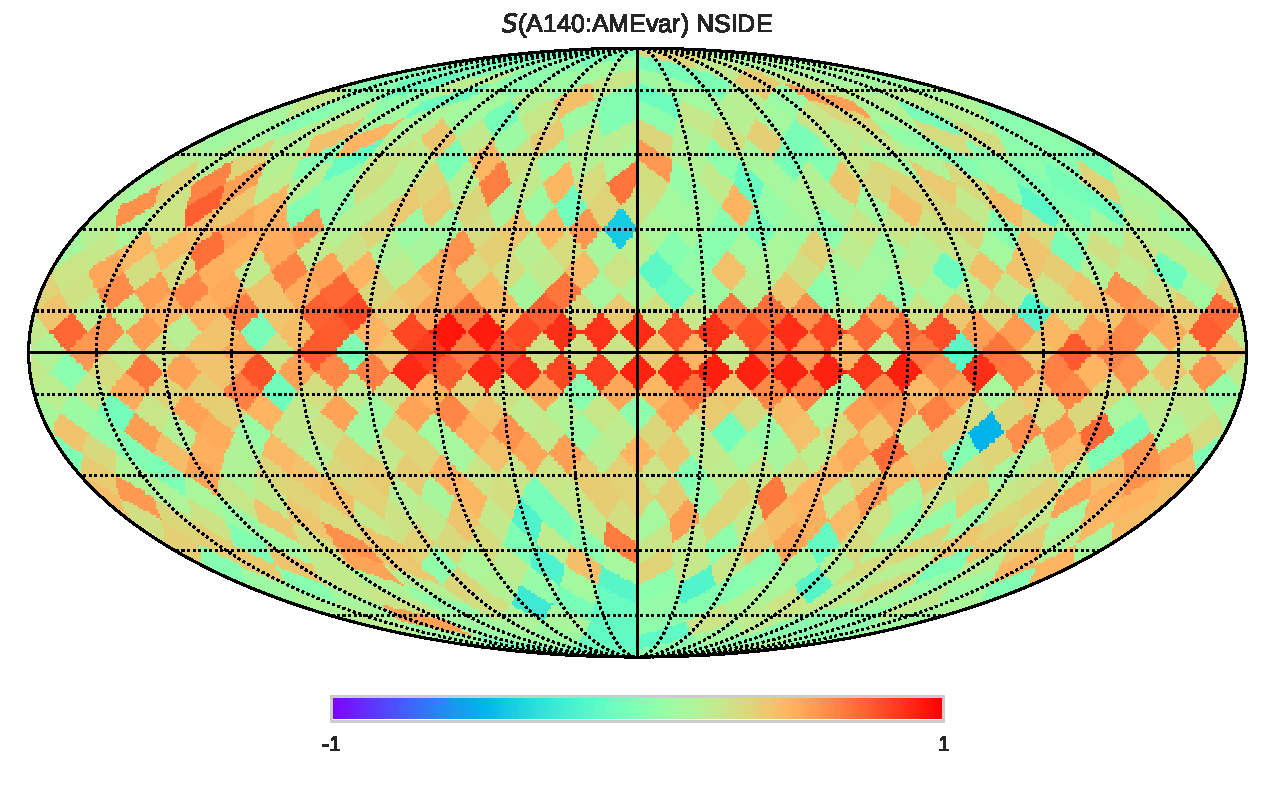
\includegraphics[width=\textwidth/2]{../Plots/Allsky_Corr/Spearman_Map_nside8_A140toAMEvar.pdf}
        \centering
        \caption{Spatial map of $r_{s}$ between the AME and IR intensity for A140, calculated as in Fig.~\ref{fig:Spearman_Map_nside8_AMEvartoIR_A9}.}
        \label{fig:Spearman_Map_nside8_AMEvartoIR_A140}
      \end{figure}
  The most important feature of these maps is that they look very similar, confirming in a spatial context that there is very little difference overall, when comparing AME to IR in intensity, accross multiple wavelengths. The correlations weaken for the MIR bands at higher latitudes, as expected. Thus the question of which band correlates better depends on exactly where we look. Considering that we need also to look at secondary correlations, not only in intensity, we repeat the above process for ratios of the MIR to AME, scaling both by $U$, as in Fig,~\ref{fig:all_bands_corr_matrix_wAME_spearmanU_norm_AMEnorm_masked} (which gave the highest correlation between MIR and AME.) Figs.~\ref{fig:Spearman_Map_nside8_AMEvartoIR_UNorm_A9}-\ref{fig:Spearman_Map_nside8_AMEvartoIR_UNorm_I25} show such correlation maps.
     \begin{figure}
       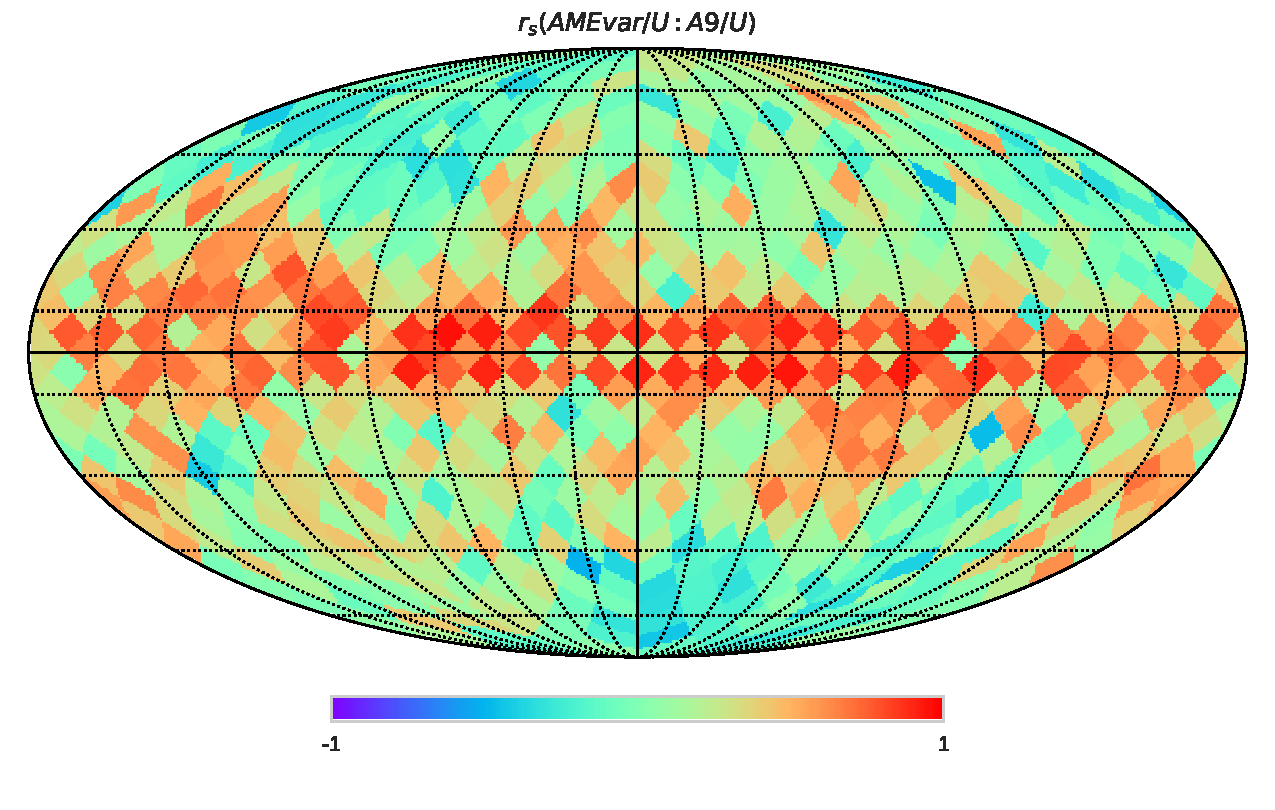
\includegraphics[width=\textwidth/2]{../Plots/Allsky_Corr/UNorm/Spearman_Map_nside8_AMEvartoA9.pdf}
       \centering
       \caption{Spatial map of $r_{s}$ between the AME:$U$ and A9:$U$, a tracer of the column density of PAHs emitting within the A9 filter. The correlations are calculated as in Fig.~\ref{fig:Spearman_Map_nside8_AMEvartoIR_A9}.}
       \label{fig:Spearman_Map_nside8_AMEvartoIR_UNorm_A9}
     \end{figure}
     \begin{figure}
       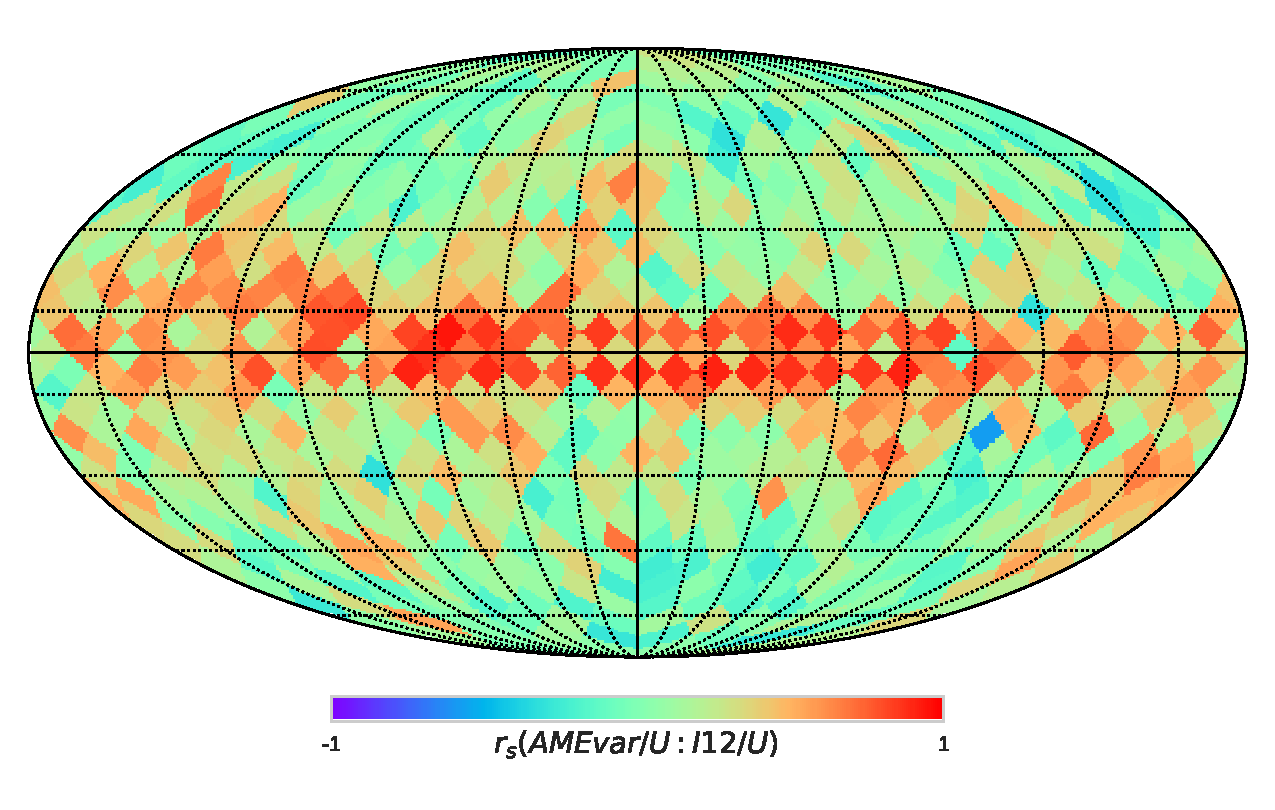
\includegraphics[width=\textwidth/2]{../Plots/Allsky_Corr/UNorm/Spearman_Map_nside8_AMEvartoI12.pdf}
       \centering
       \caption{Spatial map of $r_{s}$ between the AME:$U$ and I12:$U$}
       \label{fig:Spearman_Map_nside8_AMEvartoIR_UNorm_I12}
     \end{figure}
      \begin{figure}
        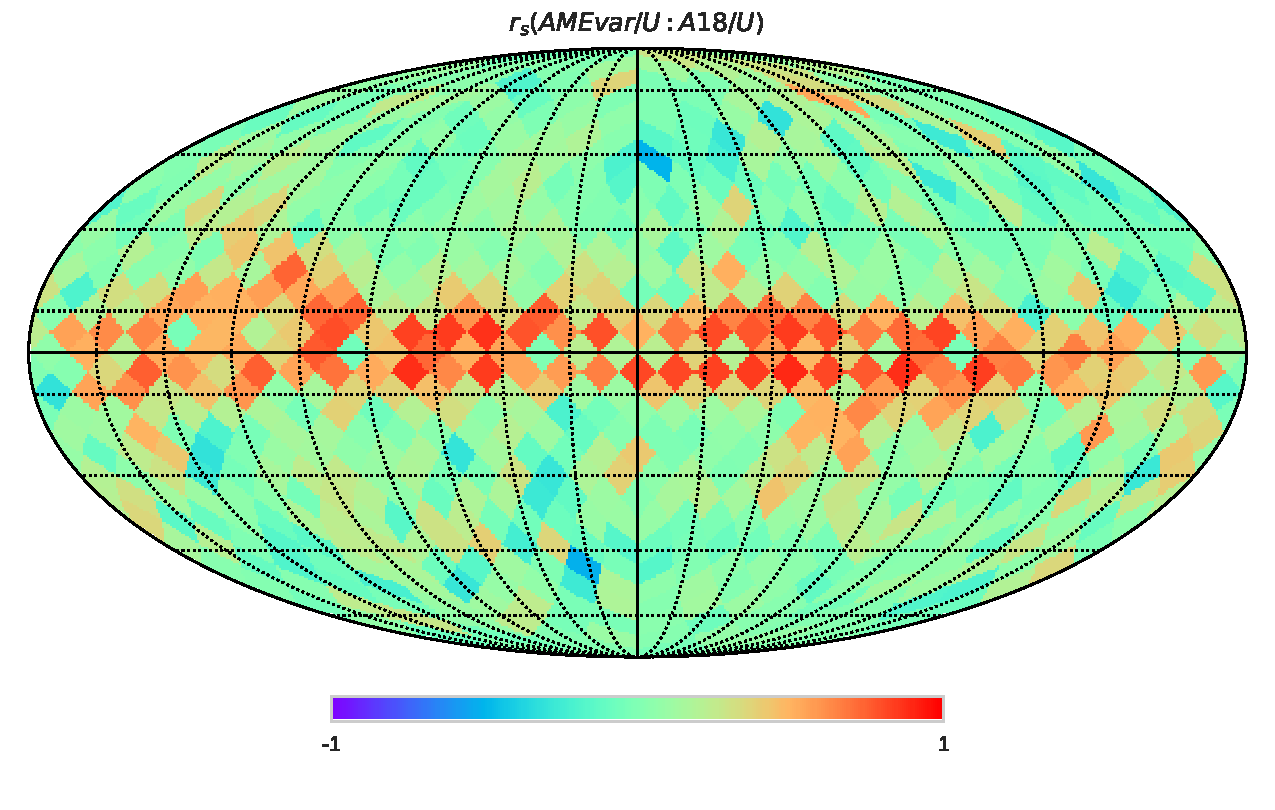
\includegraphics[width=\textwidth/2]{../Plots/Allsky_Corr/UNorm/Spearman_Map_nside8_AMEvartoA18.pdf}
        \centering
        \caption{Spatial map of $r_{s}$ between the AME:$U$ and A18:$U$}
        \label{fig:Spearman_Map_nside8_AMEvartoIR_UNorm_A18}
      \end{figure}
    \begin{figure}
         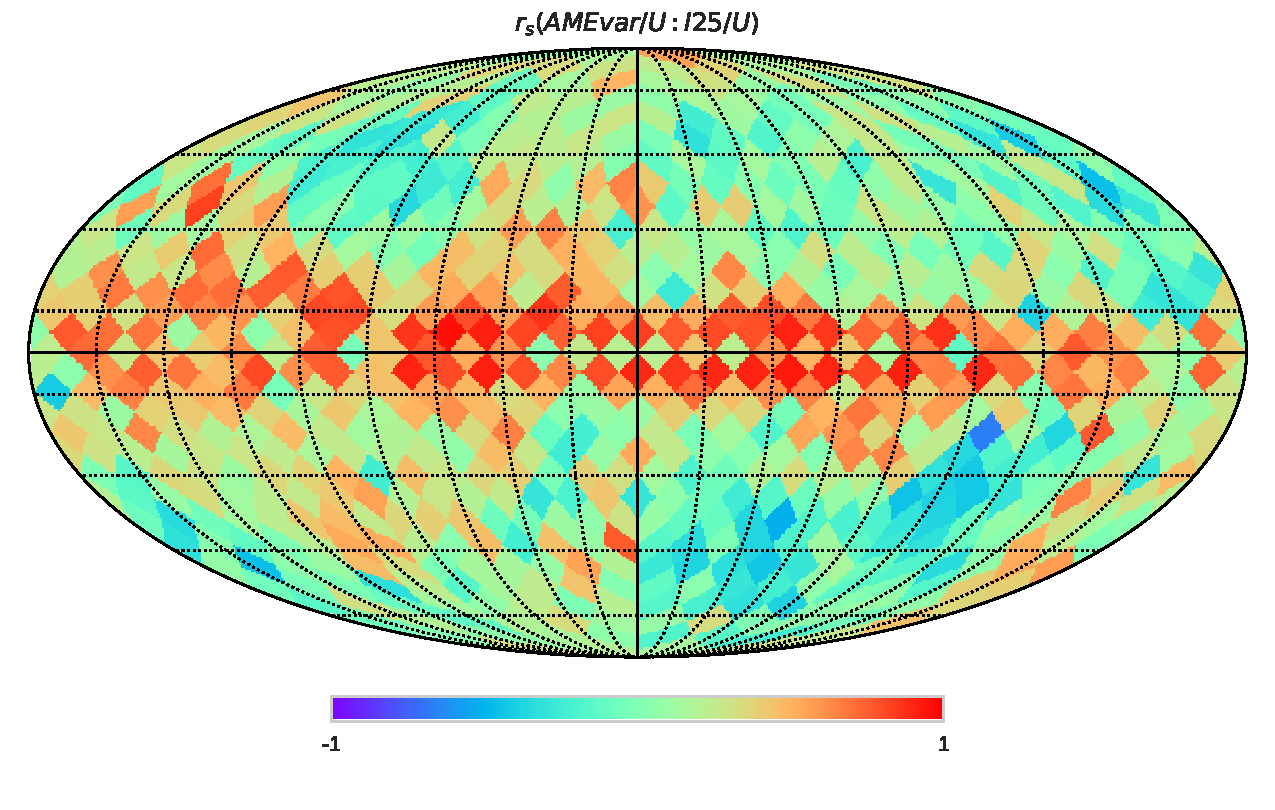
\includegraphics[width=\textwidth/2]{../Plots/Allsky_Corr/UNorm/Spearman_Map_nside8_AMEvartoI25.pdf}
         \centering
         \caption{Spatial map of $r_{s}$ between the AME:$U$ and I25:$U$}
         \label{fig:Spearman_Map_nside8_AMEvartoIR_UNorm_I25}
    \end{figure}
  Scaling by $U$ does not change the overall structure of these correlation maps, relative to the unscaled versions. This may indicate that at the scale of these correlation maps, the strength of $U$ does show much variation.
  Corresponding to Fig., we explore if the results found when looking at all of our unmasked pixels in a delocalized manner, are replicated when we produce all-sky maps of $R$-normalized intensities. These maps are indicated in Figs.~\ref{fig:Spearman_Map_nside8_AMEvartoIR_RadNorm_A9}-\ref{fig:Spearman_Map_nside8_AMEvartoIR_RadNorm_I25}.
    \begin{figure}
      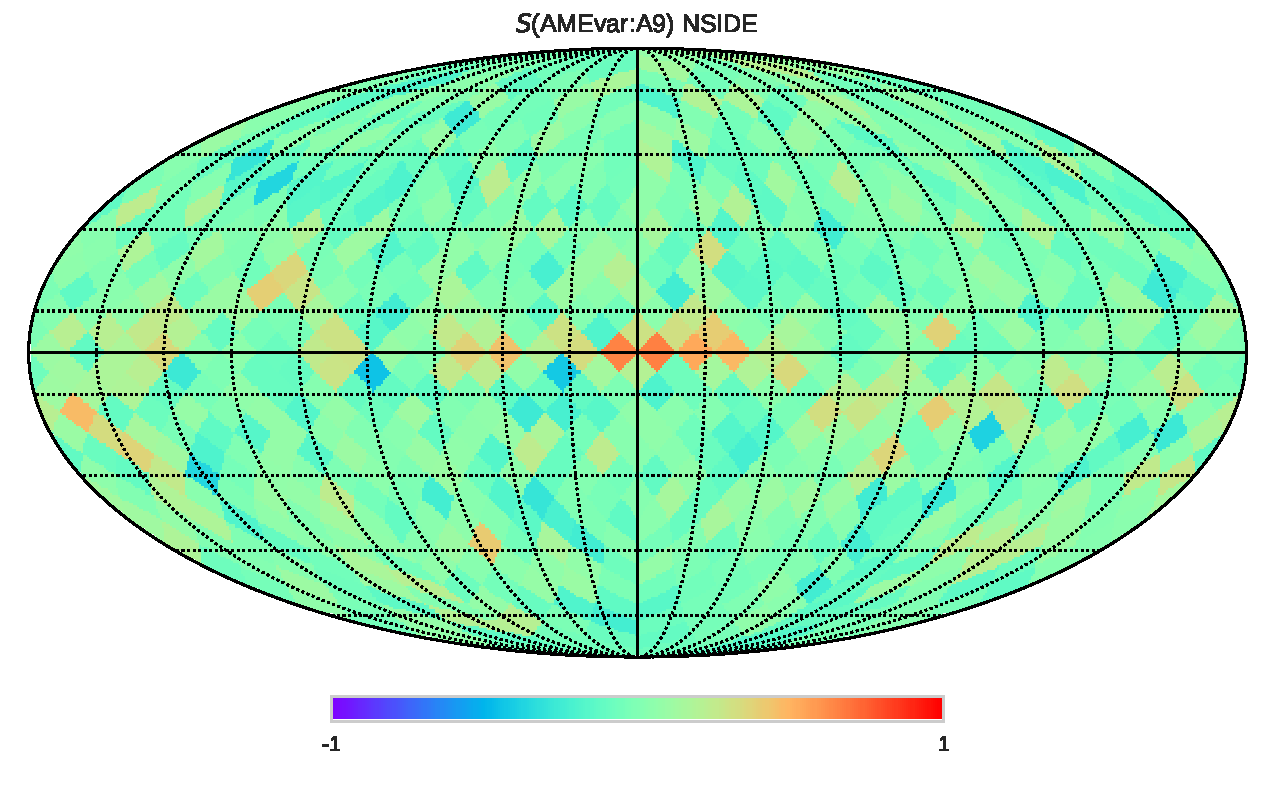
\includegraphics[width=\textwidth/2]{../Plots/Allsky_Corr/RadNorm/Spearman_Map_nside8_AMEvartoA9.pdf}
      \centering
      \caption{Spatial map of $r_{s}$ between the AME:$R$ and A9:$R$, a tracer of the fraction of dust mass in PAHS, $fPAH$. The correlations are calculated as in Fig.~\ref{fig:Spearman_Map_nside8_AMEvartoIR_A9}.}
      \label{fig:Spearman_Map_nside8_AMEvartoIR_RadNorm_A9}
    \end{figure}
    \begin{figure}
      \includegraphics[width=\textwidth/2]{../Plots/Allsky_Corr/RadNorm/Spearman_Map_nside8_AMEvartoI12.pdf}
      \centering
      \caption{Spatial map of $r_{s}$ between the AME:$U$ and I12:$U$}
      \label{fig:Spearman_Map_nside8_AMEvartoIR_RadNorm_I12}
    \end{figure}
     \begin{figure}
       \includegraphics[width=\textwidth/2]{../Plots/Allsky_Corr/RadNorm/Spearman_Map_nside8_AMEvartoA18.pdf}
       \centering
       \caption{Spatial map of $r_{s}$ between the AME:$U$ and A18:$U$}
       \label{fig:Spearman_Map_nside8_AMEvartoIR_RadNorm_A18}
     \end{figure}
   \begin{figure}
        \includegraphics[width=\textwidth/2]{../Plots/Allsky_Corr/UNorm/Spearman_Map_nside8_AMEvartoI25.pdf}
        \centering
        \caption{Spatial map of $r_{s}$ between the AME:$U$ and I25:$U$}
        \label{fig:Spearman_Map_nside8_AMEvartoIR_UNorm_I25}
   \end{figure}

    \section{Discussion}
        As noted in Ch.~\ref{ch:intro}, previous studies found that the AME generally correlates at dust-related IR wavelengths \citep{ysard10b,planckXV, hensley16}. We see the same overall pattern in the present study. We also corroborate that the FIR emission shows the tightest correlation with the AME intensity, for large portion of the sky in a de-localized fashion. In testing for a second-order correlation, we divided the IR intensities and AME intensity by $U$, and again performed the band-by-band all-sky comparison. There is evidence of a residual correlation between $I_{MIR}/U$ and $I_{AME}/U$.

       The closeness of the correlation coefficients found here is consistent with the results of the IRAS vs. AME correlation test result from \cite{planckXV}. They found that the correlation coefficient among the 4 IRAS bands (12, 25, 60, and 100~$\mu$m) differ from one another only by about 5\%, across their whole set of 98 regions. They had also indicated that many of the regions sampled were HII regions, and that free-free emission may not have been completely separated from the AME. We consider that a similar phenomenon may be happening in the PCAME map we explore here. The trend of AKARI MIR and FIR data vs. the AME does not disagree with their IRAS comparison. This work adds that individual band intensities longer than IRAS 100~$\mu$m also correlate strongly with AME, especially the two Planck/HFI bands used.


          \subsection{AME and interstellar radiation fields}
            The fact that, for our masked analysis, the best correlation between the MIR bands and AME is found with after scaling both by $U$, indicates that the AME intensity is somewhat dependent on $U$. While it is expected that AME intensity depends both on the abundance of carriers, and various excitation terms, it is not predicted that $U$ directly influences spinning dust excitation. However it may be an indirect tracer of galactic environments and various other spinning dust excitation factors. According to spinning dust theory outlined in \cite{draine98a} and in subsequent works by \cite{ysard10a}, the AME profile and intensity will depend in part on the ISRF- but as is well-stated in \cite{hensley17a}, exactly how the ISRF will affect the AME SED is a more complicated question. Absorbed starlight photons may be able to rotationally excite the carriers, but if an enhanced ISRF leads to increased dust heating, then the increased IR emission can rotationally de-excite the carriers. Moreover the ISRF affects not only the dust temperature but ionization of the carriers. The slight improvement with division by $U$ was also seen with our investigation of $\lambda$~Orionis in Ch.~\ref{ch:lori}.

          \subsection{Microwave foreground component separation}
            There are known degeneracies between the foreground parameters of the COMMANDER maps (spinning-dust, and free-free, synchrotron components as described in \cite{planck15X}.) This can be demonstrated by examing the ratio map of the PCXV intensity to thermal dust intensity, as was shown in Ch.~\ref{ch:datasources}, Fig. to the PC free-free and synchrotron maps (the PC synchrotron map shows little difference from the \cite{haslam82} 408~MHz map, is the cross-correlation plots show.) Revisiting this problem, Figs.~\ref{fig:AMEvartoDust_ffandSyncCountours} and~\ref{fig:AMEfixtoDust_ffandSyncCountours} show the $AME_{var}/R$ and $AME_{fix}/R$ ratio maps, with contours from the free-free and synchrotron maps.
                \begin{figure}
                    \includegraphics[width=\textwidth]{../Plots/ch_allsky/AMEvartoDust_ffandSyncCountours.pdf}
                    \centering
                    \caption{The ratio of $AME_{var}$ and PC dust radiance $R$, tracing fluctuations in AME per thermal dust emission. The contours trace the PC synchrotron (black) and free-free (white) components, to highlight various correlations between these components and PC AME fluctuations. Both free-free and syhncrotron can be seen to correlate and anti-correlate with the AME to dust ratio.}
                    \label{fig:AMEvartoDust_ffandSyncCountours}
                \end{figure}
                \begin{figure}
                    \includegraphics[width=\textwidth]{../Plots/ch_allsky/AMEfixtoDust_ffandSyncCountours.pdf}
                    \centering
                    \caption{The same as Fig.~\ref{fig:AMEvartoDust_ffandSyncCountours}, but with $AME_{fix}/R$ as the all-sky image.}
                    \label{fig:AMEfixtoDust_ffandSyncCountours}
                \end{figure}
             There are clearly regions where synchrotron emission correlates with excesses in AME. Some of these appear as more large scale fluctuations, mainly at higher galactic latitude. Interestingly, free-free shows agreement with both positive and negative fluctuations in both ratio maps. At high galactic latitude, free-free tends to be associated with positive fluctuations. This is supported by the fact that $AME_{fix}$ shows an improved correlation with both the $H\alpha{}$ map and the PC free-free map, perhaps suggesting confusion between spinning dust and free-free components.

             The results of the $R$ normalized cross-correlation test show that $ff/R$ shows a negative correlation with $AME/R$. This may be furher indication that the AME map, even with the mask applied from Sec.\ref{sec:pixmask}, may suffer from significant MW component confusion in some regions. It is difficult to quantify potential effects from component separation uncertainties relative to genuine correlations between microwave emission components, with the present data. However there remains the potential for such confusion to suppress evidence of any trend between AME and the actual value of $fPAH$.  The anti-correlation hear between free-free/R and AME/R may be consistent with findings in \cite{vonHausegger15} that free-free emission anti-correlates with AME, if pixels are weighted by S/N.

             Even though A9/R and I12/R do not correlate with AME/R overall, in our masked comparison, we do find some limited regions where these values do correlate. It may not

            \subsection{Comparison with $\lambda$~Orionis results}
                Results presented here do not conflict with results from Ch.~\ref{ch:lori}, except in that the findings from Fig.~\ref{fig:bootstrap_vs_AME}, wherein $r_{p}$ of A9 emission correlates better with AME than P545 emission, do not generalize to the results of this chapter (either the masked or unmasked cases.) However, in the masked all-sky comparison as well as in Ch.~\ref{ch:lori}, we find a better corrleation between A9 and AME than between I12 and AME when we subject the correlations to bootstrap resampling.

                Interestingly, the ring-structure of $\lambda$~Orionis region analyzed in Ch.~\ref{ch:lori}, does not have any apparent conterpart in the $AME/R$ ratio maps in Figs.~\ref{fig:AMEfixtoDust_ffandSyncCountours}~and~\ref{fig:AMEvartoDust_ffandSyncCountours}. The difference in our results, between the delocalized results presented in this chapter, and that of Ch.~\ref{ch:lori}, thus may be explained by variations in the component separation reliability. It is apparent that with the presently available data, there are a very limited number of regions on the sky which do not show strong free-free or synchrotron emissions, while also haivng enough S/N in the MIR, to reliably probe a relationship between PAH abundance fluctuations and AME fluctuations. $\lambda$~Orionis may be one of the exceptions, where the S/N high enough, and we are in fact able to see an improved correlation between PAHs and AME, relative to the overall dust emission to AME connection.
            \subsection{Optical depth}
              In the interpretation of results here, we have essentially operated under the assumption that MIR/PAH emisison, FIR emission, and the AME are all in the optically thin case. This is supported by the strong agreement in $r_{s}$, accross all IR bands and the AME, as presented in the correlation matrices here. (With the exception of the high-latitude, unmasked case in Fig~\ref{fig:all_bands_corr_matrix_wAME_spearman}.) Conversely, the $H{\alpha}$ data--- this emission is known to be absorbed by interstellar dust, and is the only map lacking a correlation with the others at $|\beta{}|<5$. $N{H}$ also shows a weaker correlation nearer to the galactic plane, likely influenced by saturation and/or self-absorption affects.

              However it has been demonstrated by \cite{sakon04} that the optically-thin assumption for PAH/UIR emission could lead to errors in the esimate of PAH abundance based on these emision features. Self-absorption for PAHs is another possibility.

              We do not expect the analysis presented here to suffer from such effects significantly, as we have masked the most confused lines of sight towards the galactic plane. However we cannot rule out the possibility that such optical depth effects, not only in PAH emisison but in the FIR or even AME, may weaken any potential relationship between the IR and microwave emisison from spinning grains. Such affects might also serve to explain discrepancies for our $\lambda$~Orionis result and the results in this chapter. $\lambda$~Orionis provides us a relatively clean line of sight compared to the all-sky analysis.

            \subsection{Potential for further investigations}
                Future breakthroughs in the AME may be seen if we are able to increase the number of regions with a reliable AME estimation. This can be obtained through improved synchrotron emission constraints, at higher resolutions. C-Band All Sky Survey (CBASS) at 5~GHz will be helpful in this regard \citep{irfan15}. C-BASS is expected to provide higher resolution low frequency constraints for the whole sky (48$''$ compared to 56$''$ for $H408$), with improved sensitivity (0.1$\mu$K). In terms of localized studies, it may be fruitful to consider the physical environment of each region (i.e. ionization state, gas temperature and density, other conditions indicated in \cite{draine98a, ali-haimoud10} to affect the SED shape) rather than relying of frequency-shifts to a template spectrum. More detailed exploration of PAH ionization, and other fluctuations between individual PAH features relative to variations in the AME spectral profile may also help us understand potential roles of PAHs in producing AME. However, even if we have excellent constraints on PAH emission features, synchrotron emission, free-free emission, and a powerful spinning dust SED model, the key data will be spectral coverage of the full AME profile. As noted in Ch.~\ref{ch:datasources}, the all-sky maps currently available, do not give constraints in the 10-20~GHz range. This means that lower frequency rspinning dust peaks and emissiviities are not well known. Improved understanding of AME and spinning dust therefore will require observations such as those being undertaken by the Q-U-I JOint Tenerife Experiment (QUIJOTE) project, which offers coverage between 10 and 20~GHz \citep{santos15}.

                We must also be careuful not to prematurely rule out AME explanations. The fact that we do not see a clear preferential relationship between AME and PAHs in this all-sky analysis, does not rule out a contribution by spinning PAHs to the AME. Likewise the fact that we do see a better correlation in $\lambda$~Orionis does not rule out contributions from other proposals, such as that form non-PAH small grains, or nanosilicates.

                Conversely, in the case that we are able to rule PAHs out as the AME carrier with confidence, this may imply some constraints on the PAH size distribution and dipole moment. As discussed in the theoretical work by \cite{draine98a, ali-haimoud10} and others, as well as the observational work by \cite{hensley16}, if PAHs exist in the ISM, they are very likely to be spinning rapidly. Thus if are able to confirm that they do not produce AME, this could tell us the morphology of ISM PAHs are not in an appropriate range to produce the observed AME. Spinning PAHs may be very real, even in the case that the AME comes from something else, if the PAHs are too large or lack appropriate electric dipoles.

\chapter{Summary}
  \label{ch:Summary}

  In Ch.~\ref{ch:intro} we demonstrated the both the mysteries and potential for answers revealed by all-sky observation and analysis. A paticular mystery, that of the Anomalous Microwave Emission, and the popular but yet unproven hypothesis that this AME comes from rapidly spinning tiny dust grains, perhaps PAHs, was introduced. We explained the merit of testing a spinning PAH hypothesis, while noting that spinning nanosilicates, or even magnetic dipole emission from dust have also been put forth in the literature.

  In Ch.~\ref{ch:datasources}, we overviewed a collection of infrared all-sky surveys that help us prove the dust SED from the UIR band range to the FIR, and discussed how these could help explore the AME question. We described also complimentary data and parameter maps from the Planck Collaboration that can be compared with the IR maps. Particular advantages of the PAH tracing bands, especially the A9 band, for covering not only neutral but potentially charged PAHs, were discussed in the context of AME investigation. Limitations were given for all of these data sets--- most of these boiling-down to component separation either of the Zodical light from thermal dust emission, or to the latter from other microwave foregrounds and the CMB.

  In Ch.~\ref{ch:lori} we combined and processed the data presented in Ch~\ref{ch:datasources} to investigate a particular region of the sky with relatively high S/N in all of the data, and demonstrating strong AME. We evaluated the background, noise, and contamination from systematic errors and point sources in these data, and compared them on a common resolution and grid. All of the analyses from simple correlation plots, to bootstrap analysis, to dust SED fitting suggest that A9 emisison correlates with AME better than I12 or D12- supporting PAH emisison as the source of AME, and suggesting the role of charged PAHs should be further explored. In addition we find that the bands near the thermal dust emisison peak show a weaker correlation, perhaps suggesting that harsh radiation fields may be destroying PAHs, leading to weaker AME. We also cautioned that although PAH mass correlates better than dust mass, we still see a good correlation between FIR emisison and AME (P545, P857). This raises the possibility that AME, PAHs, and cold dust are all correlated.

  In Ch.~\ref{ch:allsky} we attempted to find evidence that the result from Ch.~\ref{ch:datasources} applies even when looking at a less region-specific scale, using an all-sky analysis. However neither the full-sky unmasked case, or the case employing a mask of low S/N regions (mainly high galactic latitudes), point sources, and the galactic plane, showed a stronger correlation between PAH related emission and AME than that seen between FIR emission and the AME. We did however find that as in Ch.~\ref{ch:lori}, A9 tends to correlate with AME better than I12 or D12. We discussed apparent systemtic issues with the AME data, such as the possibility for under or over subtraction of free-free or synchrotron emission, and how these could serve to weaken evidence of any PAH or small grain correlation wiht the AME. Scaling the infrared intensities by $U$ does not change this result. We reproduce the result from \cite{hensley16} that there is not an overall correlation between PAH fraction and AME-per-dust-emisison, but expand this calculation showing that for a few limited regions on the sky there may be evidence of a correlation. We discuss how a potential variation on the optical thickness between UIR bands, FIR emisison, among other factors, could lead do a different result between $\lambda$~Orionis and the all-sky analysis. We also discuss potential observional advances that could help explore the issue further.

  Overall, using the presently available data, it is difficult to isolate the PAH-dust relationship, from the dust-AME relationship. We find throughout this work that a PAH-emission to AME correlation is readily demonstable, in intensity. A test of whether a second-order relationship exists, such that PAH emission is a better predictor of the AME than thermal dust emission, was shown to be inconclusive. One exception is that of $\lambda$~Orionis, where our results suggest that PAH mass correlates better with AME than does the total dust mass. Nevertheless we emphasize this point cautiously, because we were not able to generalize it to a larger scale (all-sky data with, effectively, a mask on the galactic plane and high latitude emission.)  We are not able to confirm or reject a ``spinning PAH'' hypothesis for the source of AME. However in $\lambda$~Orionis, and perhaps other regions yet to be examined in with dust SED fitting, we suggest that there is still ample reason to continue testing this hypothesis.

%\chapter{Summary}

  From these results, we cannot confirm or rule out a spinning-PAH hypothesis on an all-sky, 1$^{\circ}$ scale. While nanosilicates or magentic dipole emission from dust may be plausible contributors to the AME, as shown in \cite{hoang16a, hensley17a}, we do not find (at least at resolutions considered here) that PAHs can be ruled-out as a carrier. While it is true that the FIR in our study has a tighter correlation with AME than PAH-related bands, the correlation with PAH emission remains. This is true both when considering AME intensity to Either this is a coincidental correlation- PAHs and AME are both correlated with the ``actual'' carrier/s of AME, MIR phometric bands are not as good of a tracer of the actual PAH mass as we believed, or perhaps that PAHs are indeed contributing to the AME but that they are just one of multiple sources of the AME.

   If it can be shown that IR emission from non-PAH small dust particles, such as nanosilicates strongly correlates with the AME, another very interesting question would need to be addressed: why does PAH emission \textit{not} show a strong correlation? Do PAHs not have the range of dipole moments needed to produce emission in the 10 - 90 GHz range? Because, as is described in \cite{draine98a} and again in \cite{hensley17b}, such small particles should be spinning at the frequencies consistent with AME. Thus if we believe a particular class of small dust particles to exist, PAHs, nanosilicates, or otherwise- then they must be producing microwave emission, unless they do not have a permanent electric dipole.

  If there is a sufficient abundance of PAHs with an electric dipole, then we must consider the possibility that the data currently available to do not offer the necessary spatial resolution, or that the photometric bands used do not allow us to adequately separate the individual dust components (i.e. the PAH features from potential nanosilicate features) and/or microwave foreground emission components (free-free from spinning-dust.) We look forward to continued environment-resolved comparisons to investigate the potential AME-PAH (or AME-nanosilicates, iron nanoparticles) relationship in a region by region, especially given the disagreement we find between our examination of lambda Orionis and the all-sky analysis.


 This project is supported by JSPS and CNRS under the Japan--France Research Cooperative Program. We would like to give special thanks to the AME Workshop 2016 attendees and organizer, Chris Tibbs, for enlightening disucssions. Thanks also to Nathalie Ysard and Steven Gibson, and the staff of Grid, Inc. for helpful feedback.


%%%%%% appendix %%%%%%%
\appendix
\chapter*{A Note on Data Dimensionality}

While we aim to demonstrate the application of high dimensionality in these studies, we do not wish to mislead readers that we have assembled a 12-dimensional photometric dataset, simply because we have 12 wavebands. This statement may seem nonsensical at first, but makes sense when we consider the covariance of the data. Just from the outside, and our faithful belief that FIR dust emission looks something like a blackbody, or modified blackbody, or at the very least we can agree that emission from dust in thermal equilibrium would produce some sort of peaked continuum emission spanning multiple photometraic bands' width. If we agree on this point, then it follows naturally that said bands would be highly correlated with one another. This means that the number of truly independent data dimensions is not only lower than the number of bands used here, it is much lower.

Fig. \hyperref[fig:pca_intro]{\ref{fig:pca_intro}} shows the \% of variance in the data retained by the first $n$ principal components. Principal components are found essentially by first finding the covariance matrix of the input data, and then diaganolizing this matrix- the eigenvectors will be the basis vectors of each principal component. The eigenvalues will give the explained covariance per component. Applied in this manner, the components may not necessarily have a clear physical interpretation, but from a data analytics perspective we can at least assess the redundancies in our data. Thus from Fig. \hyperref[fig:pca_intro]{\ref{fig:pca_intro}}, and choosing an arbitrary covariance ``acceptable loss'' of 99\%, our photometric data set steeply reduces to 3 dimensions. The first component contains 98\% of the total variance.


\begin{figure}

  \includegraphics[width=\textwidth]{../Plots/ch_intro/pca_intro.pdf}
  \centering
  \caption{Explained variance decline for principal component analysis performed on a set of 12 all-sky infrared maps. The first three components account for over 99\% of the total variance. The PCA fit is performed on the whole sky, after whitening the data, using the ``scikitlearn }
  \label{fig:pca_intro}
\end{figure}


\singlespacing
\chapter*{Acknowledgements}
\addcontentsline{toc}{chapter}{Acknowledgements}
     I would like to thank Professor Takashi Onaka firstly for guiding me since I first came to his laboratory as an undergraduate summer intern, in June 2012. I'm not sure if I've worked hard enough for the honor of being his last Ph.D. student, but its been a pleasure. I am extremely happy that I to complete my degree here. I wish him the happies of retirements, while sincerely doubting he will be able to stay away from research for long.

     Onaka-sensei and the members of the Onaka-lab have literally helped me to survive here, assisting any time that I have had difficulty adjusting as a foreign student.

    Itsuki Sakon has helped me greatly from the moment I arrived in Japan (literally.) It is also quite refreshing when his driving skills leave me at my destination much earlier than planned.

     I have been very lucky to have helpful co-authors for the various posters and abstracts I have presented in the course of this thesis: Ho-Gyu Lee, Daisuke Ishihara, Yasuo Doi, Ho-Gyu Lee, Mark Hammonds, Fumihiko Usui, Takafumi Ootsubo, Ryou Ohsawa, Tamami Okada, Hidehiro Kaneda --- especially, my international collaborators kind enough to host me over the years, Ronin Wu, Mridusmita Buragohain, Rupjyoti Gogoi, Frederic Galliano, Amit Pathak, Martin Giard, and Olivier Berne.

     My undergraduate advisor, Steven Gibson, deserves a special thanks for continued kind encouragement and research advice even now that I have graduated from WKU.

     Most personally, I must thank my mother, Catherine Marie Bell who has supported me more than seems possible for a single human being. The same goes to my younger siblings, Joseph, Emma, Caleb, and Noah who I have too few opportunities to help grow up. I thank also Deborah and Faithie (``Mama'') Guffy, who have been like aunt and gradnmother to us all.

     My day to day life in Japan has been brightened by partner of five years, Yuki Sugisawa \begin{CJK}{UTF8}{min}(杉澤友紀)\end{CJK}. His family too, who have been an unofficial host-family over the years, Chikako \begin{CJK}{UTF8}{min}(千賀子様),Hiromi (宏美様), Takeshi (剛様), and Chiri\end{CJK}. Even his grandmother Junko and grandfather Sadao Masuda \begin{CJK}{UTF8}{min}(桝田順子と定雄様)\end{CJK} have shown me much kindness during my visits to Osaka.

     A special note of thanks is owed to my friends who have inspired me and shared moral support, from back in the US, throughout my program: Alexandria Boswell, Hannah Kagan-Moore, Alexander Chen, George Johnson, Nicolas Tarantino, and John Max Wilson; as well as my classmates at U.Tokyo, Scarlet Elgueta, Jerome de Leon, Ryouta Kawamata, Takahiro Sudoh, Taku Okamura, John Livingston, Kyle Mede, Yuta Kato, and others.

     This project could not have found its way to any assemblance of completion without kind and insightful discussions with Nathalie Ysard, Alessandra Candian,  Chikako Yasui, Norita Kawanaka, Bruce Draine, Chris Tibbs, Francois Boulanger, Brandon Hensley, Clive Dickinson, Yasushi Suto, Othman Benomar, and Anthony Jones.

     The staff of GRID, Inc., especially Mehdi Shibahara and Ying-Ming Chen, helped guide my career choices and advance my knowledge of machine learning besides being the best lunch pals.

     I wish the best of luck to my kohais in Onaka-lab: Izumi Endo, Jin Zhang, Tomoyuki Kimura, Ayato Ikeuchi, and Mingie Jian in their continued studies and careers. I also want to express special thanks to the staff of the International Liaison Office, for advising me over the last five years, even since I was an undergraduate research internship student, in the UTRIP program of 2012.

     This project acknowledges a wide range of authors. I would like also to credit especially any of those whose names did not make it into the literature, for whatever reason. Especially the many women and minorities who have made direct or indirect contribtuions to science, but have been systematically overlooked and underrepresented in journals and awards.

     My financial support for living and tuition expenses during this time has been generously provided by "MEXT", the Ministry of Education, Culture, Sports, Science and Technology (\begin{CJK}{UTF8}{min}文部科学省.\end{CJK}). This research is based on observations with AKARI, a JAXA project with the participation of ESA; Planck (http://www.esa.int/Planck), an ESA science mission with instruments and contributions directly funded by ESA Member States, NASA, and Canada; and IRAS, a joint project of the US, UK and the Netherlands.

    This research made use of Montage. It is funded by the National Science Foundation under Grant Number ACI-1440620, and was previously funded by the National Aeronautics and Space Administration's Earth Science Technology Office, Computation Technologies Project, under Cooperative Agreement Number NCC5-626 between NASA and the California Institute of Technology


\small
\bibliographystyle{apj}
\bibliography{reference}
\end{document}
